\documentclass[openany,a4paper,12pt,oneside]{book}
\usepackage{graphicx}
\usepackage{times} %pacote da fonte Times New Roman
\usepackage[top=3.5cm,left=3cm,right=3cm,bottom=2.5cm]{geometry}
\usepackage{setspace}

%regras:
%unidades não podem estar italizadas e devem estar separadas dos valores numéricos
%equações antes de um parágrafo têm que ter pontuação, como ponto no final antes de parágrafo novo e vírgula no final em caso de continuação do parágrafo.
%citações em ordem de citação, não alfabético nem essas coisas
%tentar usar 3ª pessoa mas se necessário usar 1ª pessoa é aceitável
%figuras com bons tamanhos e garantir que os labels e legendas estejam claramente legíveis
%captions devem ser bem descritivos e informativos e no texto normal deve haver uma discussão adequada com referência às imagens e tabelas

%Chapter:
%\usepackage[Bjornstrup]{fncychap}
\usepackage[T1]{fontenc}
\usepackage{titlesec, blindtext, color}
\definecolor{gray75}{gray}{0.75}
\newcommand{\hsp}{\hspace{20pt}}
\titleformat{\chapter}[hang]{\Huge}{\thechapter\hsp\textcolor{gray75}{|}\hsp}{0pt}{\Huge}
\titlespacing*{\chapter}{0pt}{-40pt}{30pt}

% Fancy headings and chapter
\usepackage{fancyhdr,titlesec,microtype}
\setlength{\headheight}{15pt}
\pagestyle{fancy}
\fancyheadoffset[L,R]{0pt}
\renewcommand{\chaptermark}[1]{\markboth{#1}{}}
\renewcommand{\sectionmark}[1]{\markboth{\thesection\ #1}{}}
\fancyhf{}
%\fancyhead[LE]{\makebox[0pt][l]{\thepage}\hfill\leftmark}
\fancyhead[R]{\rightmark\hfill\makebox[0pt][r]{\thepage}}
\fancyhead[L]{\leftmark}
\fancypagestyle{plain}{%
    \fancyhead{} % get rid of headers
    \renewcommand{\headrulewidth}{0pt} % and the line
}

%%\usepackage[brazilian]{babel}
\usepackage{amsmath}
\usepackage{amsthm}
\usepackage{amssymb}
\usepackage{amsfonts}
\usepackage{graphicx}
\usepackage{physics}
\usepackage{csquotes}
\usepackage{geometry}
\usepackage{appendix}
\usepackage{indentfirst}
\usepackage{url}
\usepackage{hyperref}
\usepackage{subcaption}
\usepackage[super]{nth}
\usepackage{siunitx}
\graphicspath{ {images/} }
\newcommand{\ts}{\textsuperscript} %superscript
\newcommand{\av}[1]{\left\langle #1 \right\rangle} %prod int ou média
\newcommand{\R}{\mathbb{R}} %simbolo reais 
\newcommand{\tensor}{\overleftrightarrow} %seta dupla do tensor
\renewcommand{\curl}[1]{\nabla \times #1} %rotacional
\renewcommand{\div}[1]{\nabla \cdot #1} %divergente

%\newtheorem{theorem}{Teorema}[section]
%\newtheorem{example}{Exemplo}[section]

\usepackage[sorting=none, style=numeric]{biblatex}
\addbibresource{bibliography.bib}



%%% TESTE %%%

\usepackage{amsmath}
\usepackage{amsthm}
\usepackage{amssymb}
\usepackage{amsfonts}
\usepackage{gensymb}
\usepackage{graphicx}
\usepackage{physics}
\usepackage{csquotes}
\usepackage{pdfpages}
\usepackage{appendix}
\usepackage{indentfirst}
\usepackage{url}
\usepackage{hyperref}
\usepackage{subcaption}
\usepackage[super]{nth}
\usepackage{siunitx}
\usepackage{tensor}
\graphicspath{ {images/} }
\newcommand{\ts}{\textsuperscript} %superscript
\newcommand{\av}[1]{\left\langle #1 \right\rangle} %prod int ou média
\newcommand{\R}{\mathbb{R}} %simbolo reais 
%\newcommand{\tensor}{\overleftrightarrow} %seta dupla do tensor
\renewcommand{\curl}[1]{\nabla \times #1} %rotacional
\renewcommand{\div}[1]{\nabla \cdot #1} %divergente

\newtheorem{theorem}{Teorema}[section]
\newtheorem{example}{Exemplo}[section]

\usepackage[sorting=none, style=numeric-comp]{biblatex}
\addbibresource{bibliography.bib}

%%% TESTE %%%

%\setlength{\abovedisplayskip}{1cm}

\title{Dissertação Mestrado}
\author{Arthur Diniz Meirelles}
\date{}

\begin{document}

\pagenumbering{gobble}

\begin{titlepage}
\pagestyle{empty}
\begin{center}

%%%%%%%%%%%%%%%%%%%%%%%%%%%%%%%%%%%%%%%%%%%%%%%%%%%%%%%%%%%%%%%%%%%%%%%%%%%%%%%%%%%%%    
%\Título da Tese \ Thesis title
	{\fontsize{16}{16} \selectfont Universidade de São Paulo \\}
	\vspace{0.1cm}
	{\fontsize{16}{16} \selectfont Instituto de Física}
    \vspace{3.3cm}

	{\fontsize{22}{22}\selectfont Vínculos cosmológicos com o auxílio do efeito Sachs-Wolfe integrado \par}
    \vspace{2cm}

%%%%%%%%%%%%%%%%%%%%%%%%%%%%%%%%%%%%%%%%%%%%%%%%%%%%%%%%%%%%%%%%%%%%%%%%%%%%%%%%%%%%%    
%\Nome do Autor \ Author's name

    {\fontsize{18}{18}\selectfont Arthur Diniz Meirelles \par}

    \vspace{2cm}

\end{center}

%%%%%%%%%%%%%%%%%%%%%%%%%%%%%%%%%%%%%%%%%%%%%%%%%%%%%%%%%%%%%%%%%%%%%%%%%%%%%%%%%%%%%%    
%\Orientador e coorientador (se existir) \ Supervisor and co-supervisor (if there is one)
\leftskip 6cm
\begin{flushright}	
\leftskip 6cm
Orientador: Prof. Dr.  Edivaldo Moura Santos \\
\leftskip 6cm
%Se não houve coorientador, comente a linha abaixo \ If there is no co-advisor, comment line below
Coorientador: Prof. Dr. Ronaldo Carlotto Batista
\end{flushright}	

    \vspace{0.8cm}    

%%%%%%%%%%%%%%%%%%%%%%%%%%%%%%%%%%%%%%%%%%%%%%%%%%%%%%%%%%%%%%%%%%%%%%%%%%%%%%%%%%%%%    
% Grau Acadêmico \ Degree

\par
\leftskip 6cm
\noindent {Dissertação de mestrado apresentada ao Instituto de Física da Universidade de São Paulo, como requisito parcial para a obtenção do título de Mestre(a) em Ciências.}
\par
\leftskip 0cm
\vskip 2cm

%%%%%%%%%%%%%%%%%%%%%%%%%%%%%%%%%%%%%%%%%%%%%%%%%%%%%%%%%%%%%%%%%%%%%%%%%%%%%%%%%%%%    
% Banca Examinadora -- Primeiro nome é do presidente ou do presidente da banca \ Examining committee -- The first name must be the supervisor's name or the examination committee president's name.

\noindent Banca Examinadora: \\
\noindent Prof(a). Dr. Edivaldo Moura Santos - Orientador (IF-USP) \\
Prof(a). Dr(a). Nome do(a) Professor(a) (institui\c{c}\~{a}o de trabalho) \\
Prof(a). Dr(a). Nome do(a) Professor(a) (institui\c{c}\~{a}o de trabalho) \\
\vspace{2.8cm}


%%%%%%%%%%%%%%%%%%%%%%%%%%%%%%%%%%%%%%%%%%%%%%%%%%%%%%%%%%%%%%%%%%%%%%%%%%%%%%%%%%%%    
%Data \ Date
\centering
    {São Paulo \\  2024}
\clearpage
\end{titlepage}



\newpage

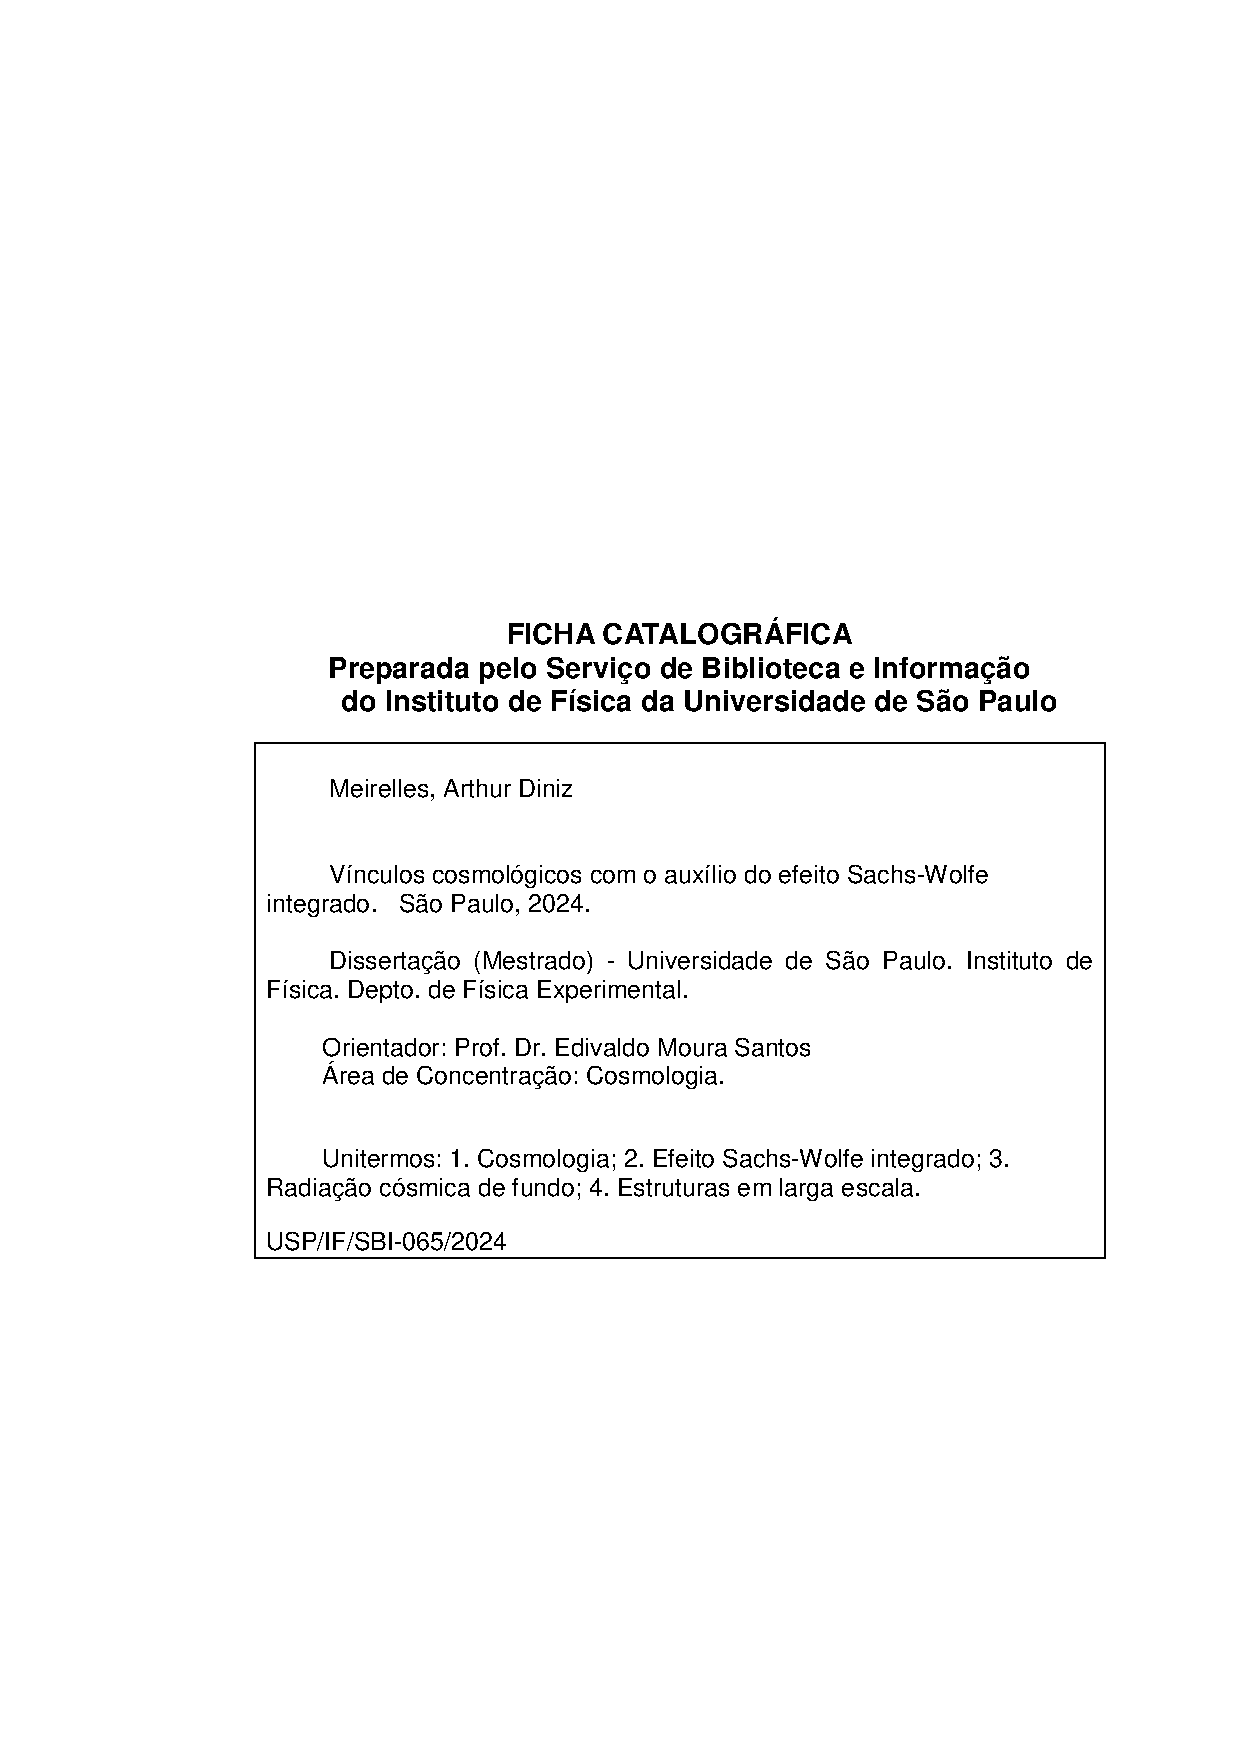
\includepdf[pages={1}]{FichaCatalog.pdf}

%\begin{center}
%\thispagestyle{empty}
%\vspace*{\fill}
%FICHA DA BIBLIOTECA
%\vspace*{\fill}
%\end{center}

\newpage

\begin{titlepage}
\pagestyle{empty}
\begin{center}

%%%%%%%%%%%%%%%%%%%%%%%%%%%%%%%%%%%%%%%%%%%%%%%%%%%%%%%%%%%%%%%%%%%%%%%%%%%%%%%%%%%%%    
%\Título da Tese \ Thesis title
	{\fontsize{16}{16} \selectfont University of São Paulo \\}
	\vspace{0.1cm}
	{\fontsize{16}{16} \selectfont Physics Institute}
    \vspace{3.3cm}

	{\fontsize{22}{22}\selectfont Cosmological Constraints using the Sachs-Wolfe Integrated Effect \par}
    \vspace{2cm}

%%%%%%%%%%%%%%%%%%%%%%%%%%%%%%%%%%%%%%%%%%%%%%%%%%%%%%%%%%%%%%%%%%%%%%%%%%%%%%%%%%%%%    
%\Nome do Autor \ Author's name

    {\fontsize{18}{18}\selectfont Arthur Diniz Meirelles \par}

    \vspace{2cm}

\end{center}

%%%%%%%%%%%%%%%%%%%%%%%%%%%%%%%%%%%%%%%%%%%%%%%%%%%%%%%%%%%%%%%%%%%%%%%%%%%%%%%%%%%%%%    
%\Orientador e coorientador (se existir) \ Supervisor and co-supervisor (if there is one)
\leftskip 6cm
\begin{flushright}	
\leftskip 6cm
Supervisor: Prof. Dr.  Edivaldo Moura Santos \\
\leftskip 6cm
%Se não houve coorientador, comente a linha abaixo \ If there is no co-advisor, comment line below
Co-supervisor: Prof. Dr. Ronaldo Carlotto Batista
\end{flushright}	

    \vspace{0.8cm}    

%%%%%%%%%%%%%%%%%%%%%%%%%%%%%%%%%%%%%%%%%%%%%%%%%%%%%%%%%%%%%%%%%%%%%%%%%%%%%%%%%%%%%    
% Grau Acadêmico \ Degree

\par
\leftskip 6cm
\noindent {Dissertation submitted to the Physics Institute of the University of São Paulo in partial fulfillment of the requirements for the degree of Master of Science.}
\par
\leftskip 0cm
\vskip 2cm

%%%%%%%%%%%%%%%%%%%%%%%%%%%%%%%%%%%%%%%%%%%%%%%%%%%%%%%%%%%%%%%%%%%%%%%%%%%%%%%%%%%%    
% Banca Examinadora -- Primeiro nome é do presidente ou do presidente da banca \ Examining committee -- The first name must be the supervisor's name or the examination committee president's name.

\noindent Examining Committee: \\
\noindent Prof. Dr. Edivaldo Moura Santos - Supervisor (IF-USP)\\
Prof. Dr. Name (institution)\\
Prof. Dr. Name (institution)\\
\vspace{2.5cm}


%%%%%%%%%%%%%%%%%%%%%%%%%%%%%%%%%%%%%%%%%%%%%%%%%%%%%%%%%%%%%%%%%%%%%%%%%%%%%%%%%%%%    
%Data \ Date
\centering
    {São Paulo \\  2024}
\clearpage
\end{titlepage}

%%%

\begin{center}
\thispagestyle{empty}
\vspace*{\fill}
\textit{Have patience with all things, but first of all with yourself.}
\vspace*{\fill}
\end{center}

%%%

\newgeometry{left=3cm, right=2cm, top=4cm, bottom=2cm,}

\begingroup
\setstretch{1}
\begin{spacing}{1.5}
\chapter*{Agradecimentos}
Este projeto, assim como qualquer outra conquista minha, não foi um trabalho individual, e sim a contribuição de um grande número de pessoas que me ajudaram, tiveram um impacto na minha vida e me influenciaram e motivaram de diversas formas diferentes, e essas influências têm tanta importância, se não mais, quanto apoios acadêmicos e financeiros. Frente à impossibilidade de dar os créditos a todos os contribuintes, tentarei me limitar aos principais.

Certamente os mais importantes são os membros da minha família, da qual todos contribuíram de alguma forma, mas eu tenho a obrigação de destacar meus pais, que lutaram contra várias adversidades para que eu chegasse onde eu cheguei, que me ensinaram o que é certo e como me dedicar, que não deixaram nada faltar a mim, e que até hoje seguem me motivando de formas diferentes, esses dois anos de muito trabalho e cansaço me fizeram ter muito mais admiração pelo esforço de ambos. Destaco ainda meus avós e minha tia Daniele, que tiveram imensa influência em quem eu sou, e contribuiram muito para a minha criação, e não posso deixar de agradecer aos meus vizinhos, Luis e Neuza, que podem não compartilhar do meu DNA, mas ajudaram a me criar como se eu fosse seus filhos, e eu tenho um imenso amor e gratidão por ambos.

Não posso deixar também de agradecer ao professor Edivaldo, que inspira a mim e a todos os seus orientandos com sua incrível competência, conhecimento, dedicação e paciência, eu acredito que esse projeto me ensinou muito além de cosmologia, e boa parte disso é graças ao senhor. Agradeço também ao professor Ronaldo, que complementou muito bem o projeto com ótimas ideias e discussões.

Outra parcela significativa dos créditos desse trabalho pertence à minha incrível namorada Carol, que está ao meu lado desde os anos em que eu era um aluno de graduação, e até antes como uma amiga muito importante, me apoiando, me inspirando e tornando meus dias melhores, mesmo que ela não perceba a influência que tem em tudo que eu faço e em quem eu sou, sobre o qual eu precisaria de muitas páginas para explicar.

Aos meus amigos, divido meus agradecimentos em duas partes: Aos que não estão envolvidos com física, pelo apoio emocional e companheirismo, pelas boas influências e motivações, e pelos bons momentos, que não deixam de contribuir para os meus esforços, deixo aqui um agradecimento especial a Pedro Augusto, que está comigo desde minha infância e até hoje tem uma grande influência na minha vida, e me presta muito apoio; e aos meus amigos que estão envolvidos com a física, não só pelos motivos citados antes, mas também por muitos momentos e discussões construtivas, pelos grupos de estudo e pelas ajudas diretas em questões acadêmicas, destaco aqui meu amigo Leonardo Lessa, que me inspirou muito durante a graduação e me inspira até hoje a estudar cada vez mais para alcançar o potencial que eu sei que tenho mas ainda não alcancei.

O presente trabalho foi realizado com apoio do CNPq, Conselho Nacional de Desenvolvimento Científico e Tecnológico - Brasil. O trabalho foi desenvolvido com recursos computacionais da Superintendência de Tecnologia da Informação da Universidade de São Paulo (USP) e do Núcleo de Processamento de Alto Desempenho (NPAD) da Universidade Federal do Rio Grande do Norte (UFRN).

\end{spacing}
\endgroup

\chapter*{Abstract}

In this work, we study the use of the Integrated Sachs-Wolfe (ISW) Effect as a tool for cosmological analysis. We do this with the use of the cross-correlation spectrum between Cosmic Microwave Background (CMB) temperature maps and galaxy contrast maps, which are used as gravitational potential tracers. We discuss how this spectrum is calculated, the influence of the galaxy redshift distribution on the correlation signal and propose a method capable of finding an optimized distribution that maximizes the cross-correlation signal, which is commonly dominated by cosmic variance, an irreducible source of fluctuation in the spectrum. With this method, we obtained a galaxy survey selection function capable of reducing in $3\%$ the the probability of compatibility with the null hypothesis, that is, a null cross-correlation signal. Furthermore, we explore the methods used to extract cross-correlation data points from masked CMB temperature and galaxy contrast maps, and use these results to calculate the likelihood profiles for the $\Lambda$CDM $\Omega_m$ parameter using WMAP's CMB temperature maps and 2MASS galaxy contrast maps for the first time in the literature. The results obtained for the likelihoods using only cross-correlation data show low constraining power. Combining the cross-correlation data with galaxy contrast autocorrelation data strongly tightens the constraints on $\Omega_m$, and all the results in this combination are compatible with Planck's best-fit parameters. We also show the likelihood profile for two synthetic cross-correlation spectra calculated, one using the $\Lambda$CDM model and the other using the value of $\Omega_m$ that maximizes the likelihood found for band 4, found for band 4 of 2MASS, both having error bars consistent with this band. The results still showed a low constraining power, but are considerably better relative to the previous ones, even when compared with the likelihood that combines all the bands.

\vspace{1cm}

\noindent \textbf{Keywords:} Integrated Sachs-Wolfe effect, cosmic microwave background, large scale structures, cosmology - observations.

\chapter*{Resumo}

Neste trabalho, estudamos o uso do Efeito Sachs-Wolfe Integrado (ISW) como uma ferramenta para análises cosmológicas. Fazemos isso utilizando o espectro de correlação cruzada entre os mapas de temperatura da Radiação Cósmica de Fundo (CMB) e mapas de contraste de galáxias, que são usados como traçadores de potenciais gravitacionais. Discutimos como esse espectro é calculado e a influência da distribuição do \textit{redshift} das galáxias no sinal de correlação, e propomos um método capaz de encontrar uma distribuição otimizada que maximize o sinal de correlação cruzada, que é comumente dominado por variância cósmica, uma fonte irreduzível de flutuação no espectro. Com esse método, obtivemos uma função de seleção capaz de reduzir em $3\%$ a probabilidade de compatibilidade com a hipótese nula, isto é, nenhum sinal de correlação cruzada. Além disso, exploramos os métodos usados para obter dados de correlação cruzada a partir de mapas mascarados de temperatura da CMB e de contraste de galáxias, e usamos esses resultados para calcular os perfis de \textit{likelihood} para o parâmetro $\Omega_m$ do modelo $\Lambda$CDM usando os mapas de temperatura da CMB do WMAP e o catálogo de galáxias 2MASS pela primeira vez na literatura. Os resultados obtidos para as \textit{likelihoods} usando apenas dados de correlação cruzada apresentam fraco poder de vínculo. A combinação dos dados de correlação cruzada com os dados de autocorrelação do contraste das galáxias fortalece os vínculos sobre $\Omega_m$, e todos os resultados dessa combinação são compatíveis com os do Planck. Também mostramos a \textit{likelihood} para dois espectros de correlação cruzada sintéticos, um usando o modelo $\Lambda$CDM e o outro usando o valor de $\Omega_m$ que maximiza a \textit{likelihood} encontrada para a banda 4, ambos com erros iguais aos da banda 4. Os resultados ainda mostram um baixo poder de vínculo, mas é constatada uma melhoria considerável em relação aos resultados anteriores, mesmo quando comparados à likelihood que combina todas as bandas.

\vspace{1cm}

\noindent \textbf{Palavras-chave:} Efeito Sachs-Wolfe integrado, radiação cósmica de fundo, estruturas em larga escala, cosmologia - observações.

%\chapter*{List of Figures}

\listoffigures

%\chapter*{List of Tables}

\listoftables

\tableofcontents

\cleardoublepage
\pagenumbering{arabic}

\begingroup
\setstretch{1}
\begin{spacing}{1.5}
\setlength{\abovedisplayskip}{0.01cm}
\setlength{\abovedisplayshortskip}{0.01cm}

\chapter{Introduction}

The discovery of the Cosmic Microwave Background (CMB) is a fine example of serendipity. Arno A. Penzias and Robert W. Wilson found an unexpected excess temperature while measuring the effective noise temperature with a microwave antenna as a function of zenith in 1964. After some investigation, they attributed this excess temperature to an isotropic radiation field that today we call the CMB \cite{1965CMB_discovery}, based on previous predictions of a remnant radiation field made by Ralph Alpher and Robert Herman \cite{1948_pred_CMB}. The CMB has since been used as one of the main probes to studying cosmology, being able to provide various tests and insights into cosmological models \cite{Large_scale_anomalies, nongaussianity_inflation, rees_sciama_effect} and measurements of cosmological parameters \cite{WMAP_results, Planck_results}. 

In the concordance cosmological model, commonly called the $\Lambda$CDM model, the Universe was very compact and energetic at its very early stages, and has always been in expansion, resulting in a reduction in overall energy density. Eventually, when it reached temperatures of around \SI{4000}{\kelvin}, photons decoupled from electrons and protons, which made possible for photons, with a blackbody spectrum, to essentially free stream across the Universe ever since \cite{CMB_physical_explanation}. The current measurement for the black body spectrum temperature of the CMB is \SI{2.72548 \pm 0.00057}{\kelvin} \cite{CMB_temperature:Fixsen_2009}, containing very small anisotropies in the order of $\SI{e-5}{\kelvin}$, which is expected in the $\Lambda$CDM model \cite{CMB_analytical_anisotropies}. These fluctuations are the result of physical effects at work during the earliest moments of the cosmos or are acting on the photons as they travel through the Universe, making them an excellent probe to constrain cosmological parameters.

Some mappings of the CMB were carried out in the last few decades. The first satellite launched specifically dedicated to doing this was the Cosmic Background Explorer (COBE) satellite with a $7\degree$ angular resolution \cite{COBE}, followed by the Wilkinson Microwave Anisotropy Probe (WMAP) with a $0.3\degree$ angular resolution, which was also able to show that CMB photons are polarized, a property related to other physical effects that assisted cosmologists in further understanding the history of the Universe \cite{polarization_1997, polarization_2014, BMode_constraints}. In 2009, the Planck Satellite was launched, improving upon WMAP's precision to an impressive value of 5' ($\sim 0.083\degree$) angular resolution \cite{theplanckcollaboration2006scientific}, allowing cosmologists to access the finest details in the CMB anisotropies to this day. Figure \ref{fig:cmb_satellites} shows a comparison between the resolution of these maps.

\begin{figure}
    \centering
    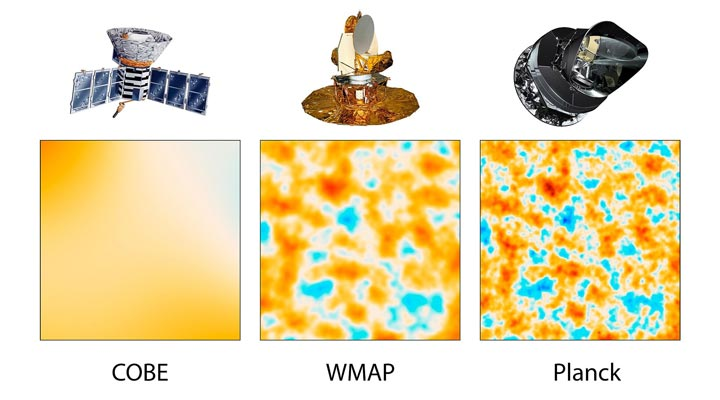
\includegraphics[width=.9\linewidth]{Imagens/satellites.jpg}
    \caption{Each image represents the same 10 square degree patch of the sky measured by the three telescopes shown above each image. The improvement in the resolution of each map is very noticeable. Credit: \href{https://lambda.gsfc.nasa.gov/education/graphic_history/microwaves.html}{NASA/LAMBDA Science Team}.}
    \label{fig:cmb_satellites}
\end{figure}

Amongst the many physical processes that affect the CMB, the Integrated Sachs-Wolfe (ISW) Effect is one of the most important. First described by Rainer K. Sachs and Arthur M. Wolfe in 1967, the ISW effect is a mechanism that causes CMB photons to blueshift or redshift in cosmological periods when gravitational potentials change rapidly. One such period is the time between the previous matter-dominated era and the current dark energy-dominated one. During this transition, gravitational potentials decay (or "flatten") over time, causing CMB photons that entered potential wells with a certain gravitational blueshift to leave these wells with a redshift that does not compensate for the initial blueshift, leaving a net temperature gain in these photons, therefore, creating patterns that can be observed in the CMB temperature map and spectrum \cite{Sachs:1967er}. The mechanism is illustrated in Figure \ref{fig:ISW_illustration}.

\begin{figure}[!htb]
	\centering
	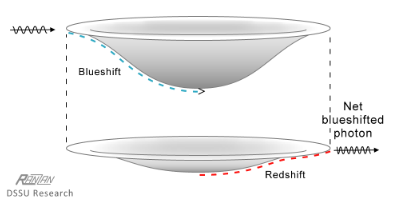
\includegraphics[width=.7\linewidth]{Imagens/ISW_illustration.png}
	\caption{Illustration of the Integrated Sachs-Wolfe Effect, in which a photon is shown entering a deep gravitational well that flattens with time, leaving the photon with a net blueshift. Credit: \href{http://www.cellularuniverse.org/SachsWolfe-Disproof(ijass)-Ranzan.pdf}{DSSU Research}.}	
	\label{fig:ISW_illustration}
\end{figure}

%There are two contributions to the ISW effect: The early-time ISW effect occurs immediately after the last scattering surface, and the late-time ISW effect, which is more recent, occurring in the transition to the current dark energy dominated era. 

From this association between blueshifted CMB photons and gravity wells, it is natural to assume that the matter distribution of the Universe should hold a statistical cross-correlation with the CMB temperature map. When looking at the theoretical model, we will see that this cross-correlation is expected \cite{ISW_detect_Crittenden1996, ISW_detect_Cooray2002}, and many works in the past have reported detections of the ISW effect using such cross-correlation of various sources of data and statistical methods \cite{ISW_detect_Boughn2004, ISW_detect_Nolta2004, ISW_detect_Gaztanga2006, ISW_detect_and_review2011}. Overall, the ISW signal was favored in these works, but mostly with low significance levels. We highlight the results shown in \cite{cross_corr:Planck}, in which many large scale structure tracers were combined to obtain a $4\sigma$ detection, from which the two main contributors were Planck's convergence lensing maps (Kappa) and the NRAO VLA Sky Survey (NVSS) \cite{NVSS}.

The present work uses the Bayesian methods presented in \cite{Moura-Santos_2016} to estimate cross-correlation spectra using CMB temperature maps from WMAP \cite{WMAP_results,WMAP_data} and galaxy contrast maps provided by the Two Micron All Sky Survey (2MASS) \cite{2MASS}, and study the constraint power of the results over a specific cosmological parameter. We have also investigated the impact of the redshift distribution of the galaxies in the catalog used on the resulting cross-correlation spectrum, and studied what would be the distribution that optimizes the signal.  

The rest of this dissertation will be organized as follows: In Chapter \ref{chapter:model}, we start by presenting the fundamental observations and principles of cosmology, some of its fundamental equations, and discuss what makes up the $\Lambda$CDM model. We first describe the universe in terms of a homogeneous and isotropic background and later introduce perturbations to this background, which allows us to determine the linear differential equations that describe the energy contents of the universe. We then focus on the radiation equation to describe the statistical distribution of the CMB today, finally reaching a point where we can mathematically define the ISW effect and its properties, as well as discuss the so called cosmic variance, a source of irreducible fluctuations in the signal. Finally, we discuss how alternative dark energy models can influence our observables.

In Chapter \ref{chapter:select_func_optimal}, we study how the redshift distribution of galaxy catalogs are generally parametrized, the general properties of such parametrization and the redshift dependence of the selection function of the four bands in the 2MASS catalog. In order to maximize the cross-correlation signal taking into account the high cosmic variance, we define the probability that a certain cross-correlation function calculated from a certain galaxy distribution is compatible with a null cross-correlation model and determine the hypothetical galaxy survey selection function parametrization that minimizes this probability. More precisely, we minimize the consistency with the null hypothesis.

In Chapter \ref{chapter:extracting_correlations_from_data}, we briefly discuss some of the properties of the data obtained from the sattelites and some traditional methods used to process that data, motivating the discussion about the Monte Carlo method used in this work. The WMAP and 2MASS data are described, the final maps used are shown, as well as the results for the correlation spectra obtained from these maps, evincing the role of cosmic variance.

Finally, in Chapter \ref{chapter:constraints}, the method used to calculate the contraints on the cosmological parameter $\Omega_m$ -- defined in Chapter \ref{chapter:model} -- from the correlation spectra is discussed. For the first time in the ISW literature, we have obtained cosmological constraints using cross-correlation data between CMB temperature maps and galaxy contrast maps. We studied these constraints not only for the four 2MASS bands, but also for a synthetic dataset generated based on the idealized galaxy redshift distribution found in Chapter \ref{chapter:select_func_optimal}. 

We summarize all the results from this project in Chapter \ref{chapter:conclusions}, draw some conclusions based on this and other works that have studied the same problem in various different ways, and present future perspectives.

\chapter{Cosmology's Concordance Model}\label{chapter:model}

The advent of general relativity in the early 20th century allowed physicists to conceptualize mathematical models of the cosmos. Albert Einstein proposed a model for a static Universe using his theory \cite{Einstein:1917ce}, and other cosmological models were proposed in the following years. To start this chapter, the fundamental principles of cosmology will be discussed and used to setup a simple background for the Universe, and the specificities of the currently most accepted model for the cosmos -- the $\Lambda$CDM model -- will be discussed. After this, we will complement this simple background with finer details and provide a statistical description of cosmological observables that can be used to test our models.

\section{The Homogeneous Background}

\subsection{Fundamental Observations and Principles}

One of the fundamental principles of cosmology is called the Cosmological Principle: at large scales, the Universe is both homogeneous and isotropic. This principle can be used to simplify the description of the energy distribution in the Universe, but it also simplifies the possible metrics that can describe the cosmos to those that have constant curvature (a quantity denoted as $k$), and it can be shown that any space with constant curvature is locally isometric to: the Euclidian flat space ($k=0$), a hyperspherical space ($k=+1$) or a hyperbolic space ($k=-1$) \cite{choquet2008general}. The Cosmological Principle has support from a good amount of cosmological observations, such as the CMB \cite{COBE}, the the spatial distribution of galaxies \cite{galaxy_isotropy, galaxy_homogeneity_Pandey_2021}, amongst others. 

In the period from 1927 to 1929, Edwin Hubble and Georges Lemaître, amongst other scientists, greatly contributed to the current understanding of cosmology. Observations were carried out and showed that most galaxies and nebulae data show a redshift proportional to their distances relative to the Earth \cite{hubble}, these results were studied using general relativity and cosmological models at the time \cite{Lemaitre:1927zz}. The results lead to idea of an expanding, i.e. non-static,  universe. In an expanding universe, it is straightforward to find a linear relationship between the redshift of the object and its distance, when that distance is not too large.

Furthermore, data show that the Universe's expansion is currently accelerated \cite{Riess_1998, Perlmutter_1999}, which is a property described differently in many cosmological models. The simplest way to account for it is by introducing a cosmological constant $\Lambda$ in Einstein's field equations.

After adopting a coordinate system, in order to describe the dynamics of the Universe, one introduces a scale factor $a$, whose present value is 1 (usually called $a_0$) and at any given time, $a(t)$ represents the size of the Universe with respect to its present size. A simple relation can be established between the scale factor of an observed object and its redshift $z$:

\begin{equation}\label{1+z}
    1+z=\frac{\lambda_{\text{obs}}}{\lambda_\text{emit}}=\frac{a_\text{obs}}{a_\text{emit}}=\frac{1}{a_\text{emit}}
\end{equation}

\noindent where $\lambda$ and $a$ are the wavelength of the radiation and the scale factor, respectively, when emitted ($\lambda_\text{emit}$ and $a_\text{emit}$) and when observed ($\lambda_\text{obs}$ and $a_\text{obs}$). It is also useful to describe the expansion rate of the universe using the Hubble parameter $H(t)$ at a given time $t$

%At different times in the universe's history, the scale factor behaves differently, so it is useful to define the Hubble parameter $H(t)$ for a given cosmological time $t$:

\begin{equation}\label{def:H(t)}
    H(t)=\frac{1}{a}\dv{a}{t}.
\end{equation}

These properties are not exclusive to a particular cosmological model, instead being present in all of them. The standard model of cosmology, called $\Lambda$CDM, usually takes a few assumptions on top of the ones described previously:

\begin{itemize}
    \item During the very early stages of the Universe, it was very compact and energetic, and eventually it went through a period of rapidly accelerated expansion, called the inflationary period, which was driven by one or more scalar quantum fields;
    \item Aside from baryonic matter, radiation and neutrinos, there are two other main components in the Universe: non-relativistic (cold) dark matter and an energy component with constant density called dark energy, which is related to a cosmological constant $\Lambda$;
\end{itemize}

%Although the universe is predominantly uniform, it contains both inhomogeneities and anisotropies in its finer details that need to be studied. The traditional approach is to first set up a homogeneous background and study its properties, which is the task of this section, and then add perturbations to this background to solve for the precise statistical behavior of the universe, which will be done in the section after this one.

Based on the Cosmological Principle, most theoretical models first set up a homogeneous and isotropic background description of the Universe, and then introduce perturbations to this background, allowing for a detailed statistical description of its evolution. In the rest of this section, we will use the principles and assumptions just presented to set this background.

\subsection{Friedmann Equations}

As already mentioned, the main theoretical framework to describe the Universe is the theory of general relativity, since the most relevant force in the scale of the Universe is the gravitational one. We then use Einstein's field equations with a cosmological constant $\Lambda$:

\begin{equation}\label{field_eqs}
    R_{\mu\nu}-\frac{1}{2}g_{\mu\nu}R+\Lambda g_{\mu\nu}=8\pi GT_{\mu\nu},
\end{equation}

\noindent where $R_{\mu\nu}$ is the Ricci curvature tensor for the Universe's metric $g_{\mu\nu}$, $R\equiv g_{\mu\nu} R^{\mu\nu}$ is the Ricci scalar, $G$ is the gravitational constant and $T_{\mu\nu}$ is the energy-momentum tensor. 

In equation \eqref{field_eqs} and throughout this text (unless otherwise stated), we will use units such that the Boltzmann constant ($k_B$), the speed of light in a vacuum ($c$) and the reduced Planck constant ($\hbar$) are all equal to one. Furthermore, Greek letter tensor indices indicate that the time component of the tensor is included in the equation and Latin letter tensor indices indicate that only spatial components are included. Current results strongly indicate the metric $g_{\mu\nu}$ of the Universe to be flat ($k=0$)\cite{Planck_results}, thus justifying the use of an Euclidian metric scaled by $a(t)$, and we will assume a homogeneous and isotropic distribution of energy throughout the Universe to construct an energy-momentum tensor with constant energy density $\rho_0$ and constant pressure $P$ \cite{dodelson2020modern}:

\begin{align}\label{cap2:initial_tensors}
    g_{\mu\nu}&=
    \begin{pmatrix}
        -1 & 0 & 0 & 0\\
        0 & a^2 & 0 & 0\\
        0 & 0 & a^2 & 0\\
        0 & 0 & 0 & a^2
    \end{pmatrix} &
    T_{\mu\nu}&=
    \begin{pmatrix}
        -\rho_0 & 0 & 0 & 0 \\
        0 & P & 0 & 0 \\
        0 & 0 & P & 0 \\
        0 & 0 & 0 & P
    \end{pmatrix}.
\end{align}

The metric $g_{\mu\nu}$ described in equation \eqref{cap2:initial_tensors} is called the Friedmann-Lemaître-Robertson-Walker (FLRW) metric \cite{FLRW_metric}. 

%In order to expand any equation from \eqref{field_eqs}, it is necessary to determine $R=g^{\mu\nu}R_{\mu\nu}$. By expanding the expression using the matrices defined in \eqref{cap2:initial_tensors}, the result is

%\begin{equation}\label{riemann_constant}
%    R=6\left[\frac{\Ddot{a}}{a}+\left(\frac{\dot{a}}{a}\right)^2\right].
%\end{equation}

From all the equations in \eqref{field_eqs}, if the one corresponding to $\mu=\nu=0$ is worked out, one obtains

\begin{equation}\label{fried1_step1}
    \left(\frac{\dot{a}}{a}\right)^2=\frac{1}{3}\left(8\pi G\rho_0+\Lambda\right),
\end{equation}

\noindent which relates the relative rate at which the Universe is expanding with the energy content of the Universe. In the $\Lambda$CDM model, $\Lambda$ is assumed to be the source of the current accelerated expansion of the Universe, so an energy component related to this constant is necessary, and its energy density can be defined as

\begin{equation}\label{def:rho_lambda}
    \rho_\Lambda=\frac{\Lambda}{8\pi G},
\end{equation}

\noindent such that

\begin{equation}\label{fried_first_eq}
    \left(\frac{\dot{a}}{a}\right)^2=\frac{8\pi G}{3}\rho,
\end{equation}

\noindent where $\rho=\rho_\Lambda+\rho_0$. This is called Friedmann's first equation. 

When any of the space-space equations of \eqref{field_eqs} is expanded and the resulting equation is combined with equation \eqref{fried_first_eq}, Friedmann's second equation is obtained:

\begin{equation}\label{fried_second_eq}
    \frac{\Ddot{a}}{a}=-\frac{4\pi G}{3}(\rho+3P).
\end{equation}

This equation is a relation between the acceleration of the Universe and its energy content. It is clear that $P<-\frac{1}{3}\rho$ indicates a Universe expanding with a positive acceleration, which is highly unexpected since gravity is an attractive force, but in section \ref{subsect:Ch2_Energy_Content} the case of the cosmological constant will be discussed, in which $\Lambda$ yields $P_\Lambda=-\rho_\Lambda$, being the reason it contributes to an accelerated expansion.

\subsection{Energy Content}\label{subsect:Ch2_Energy_Content}

To understand the contribution of each component of the Universe to its dynamics, a differential equation for each component has to be determined, we do this using the energy-momentum conservation equation:

\begin{equation}\label{energy_momentum_conservation}
    \nabla_\mu T^\mu_\nu\equiv \partial_\mu T^\mu_\nu+\Gamma^\mu_{\alpha\mu}T^\alpha_\nu-\Gamma^\alpha_{\nu\mu}T^\mu_\alpha=0.
\end{equation}

Again using the energy-momentum tensor defined in \eqref{cap2:initial_tensors}, the following equation is obtained:

\begin{equation}\label{cap2:energy_conservation}
    \pdv{\rho}{t}+\frac{\dot{a}}{a}(3\rho+3P)=0.
\end{equation}

To solve this, a relation between density and pressure for each component of the Universe is needed, an equation of state. It is commonly assumed that, for a given component $s$ of the Universe, its equation of state takes the form

\begin{equation}\label{ch2:eq_state}
    P_s=w_s\rho_s,
\end{equation}

\noindent where $w_s$ is called the equation of state parameter. Using that equation and solving for $\rho_s(a)$ on equation \eqref{cap2:energy_conservation} yields

\begin{equation}\label{ch2:rho_s(a)_general}
    \rho_s(a)\propto \text{exp}\left[-3\int_1^a \frac{da'}{a'}[1+w_s(a')]\right].
\end{equation}

This solution ignores further interaction between components, it would apply to a single-component Universe, but it is also a useful first approximation in epochs of dominance of a single component. In the $\Lambda$CDM model, it is assumed that all components of the Universe possess a constant value for $w_s$, in that case the solution is simple:

\begin{equation}\label{ch2:rho_s_ws_const}
    \rho_s(a)\propto a^{-3(1+w_s)}.
\end{equation}

\noindent This represents the evolution of the density parameter of any component as a function of the scale parameter, and thus as a function of cosmological time, since $a(t)$ is monotonically increasing (the Universe has not reduced at any point in its history so far).

The rigorous form of determining $w_s$ for some components of the Universe requires the usage of statistical physics. In cases where we have limited information on the physical properties of a certain component, such as dark energy, theoretical frameworks and assumptions have to be used, as well as the analysis of data.

In the case of dark energy, assuming its origin is related to the cosmological constant, the value of $w_\Lambda=-1$ is expected, which also indicates a constant density for dark energy. From the quantum field theory point of view, the cosmological constant energy density would be associated to zero point energy of a quantum field. However, so far, no calculation has been successful in predicting a zero point energy whose density is consistent with the cosmological observations \cite{Weinberg_Lambda_1989}. Many models propose alternative possibilities, the simplest being a constant equation of state parameter $w_{DE}$ that might not be $-1$, while other options assume dark energy to be dynamical, meaning $w_{DE}$ is a function of $a$ \cite{DE_models}, which would still be able to explain the accelerated expansion of the Universe as long as $w_{DE}<-\frac{1}{3}$. Recent preliminary results reported by DESI have found statistical preferences of $2.6\sigma$ to $3.9\sigma$ towards such models\cite{DESI2024}, which will be discussed in more detail in section \ref{sect:dark_energy}. Table \ref{tab:rhos&Omegas} summarizes the equation of state properties of each known component in the Universe. %Recent preliminary results assuming this $w$CDM scenario have found values marginally compatible with $w_\Lambda$ \cite{DES2024}. 

It is very useful to also define the energy density fraction of each component of the Universe using

\begin{equation}\label{eq:Omega_def}
    \Omega_s=\frac{\rho_s(a_0)}{\rho_\text{crit}},
\end{equation}

\noindent where $\rho_\text{crit}$ is the so called critical density, defined as

\begin{equation}\label{def:rho_crit}
    \rho_\text{crit}\equiv \frac{3H_0^2}{8\pi G}\approx \SI{8.5e-27}{\kilogram /\meter^{3}},
\end{equation}

\noindent where $H_0$ is the Hubble constant, the value of the Hubble parameter $H(t)$ defined in \eqref{def:H(t)} at the present.

This energy density makes it possible to determine what is the curvature of the Universe: if the total sum of energy densities in the Universe is equal to the critical one, the Universe is flat; if this sum is higher than $\rho_\text{crit}$ the Universe would have positive curvature; and if this sum is lower than $\rho_\text{crit}$, the Universe would have negative curvature \cite{schutz2009first}. 

Table \ref{tab:rhos&Omegas} summarizes the current estimated values for these energy fractions for the Universe in the present. It is important to note that commonly in cosmology (and throughout this text), the classification of baryons includes electrons, even though, according to the standard model of particle physics, electrons belong, together with their associated neutrinos, to one of the three families of leptons.

\begin{table}[!htb]
\centering
    \begin{tabular}{cccc} \hline
     Component & $\rho(a)$ & $w$ & $\Omega$ \\ \hline
     Baryonic matter ($\Omega_b$) & $\rho_0a^{-3}$ & $0$ & $0.0493\pm 0.0009$\\
     Cold dark matter ($\Omega_c$) & $\rho_0a^{-3}$ & $0$ & $0.2645 \pm 0.0050$ \\
     Radiation ($\Omega_r$) & $\rho_0a^{-4}$ & $\frac{1}{3}$ & $5.29\times 10^{-5}$\\
     Dark energy ($\Omega_\Lambda$) & $\rho_0$ & $-1$ & $0.6847\pm 0.0073$\\
     Curvature ($\Omega_k$) & $\rho_0 a^{-2}$ & $-\frac{1}{3}$ & $0.001\pm 0.002$\\ \hline
    \end{tabular}
    \caption{Equation of state parameters $w$, energy density functions $\rho(a)$ and energy density fractions for each known component of the Universe according to the $\Lambda$CDM model. Most data were adapted from Planck \cite{Planck_results}, the radiation data was calculated based on \cite{lahav2014cosmological}.}
    \label{tab:rhos&Omegas}
\end{table}

\subsection{A Brief History of the Universe}

We commonly categorize different stages of the Universe according to important events that happened during its history. The $\Lambda$CDM model assumes the Universe started as a singularity; as it started expanding, quantum fluctuations at that time would eventually result in inhomogeneities thought to be the source for the formation of structures.

The next important period of the Universe's evolution was a highly accelerated expansion epoch driven by an effect called cosmic inflation, first proposed as a solution to the horizon problem \cite{Guth81,linde82}, related to how the CMB temperature differences across the sky can be so small ($\sim 10^{-5}$ K), even between points apparently causally disconnected during all epochs of the Universe's thermal history. The $\Lambda$CDM model assumes inflation was driven by a quantum scalar field \cite{dodelson2020modern}. Definitive evidence of the inflationary model could be obtained with the detection of the so called B-modes of the CMB polarization. Searches for primordial B-modes in the last decade are leading to strong constraints on the contribution to the CMB polarization spectrum \cite{BMode_constraints}.

Briefly after inflation, baryons and photons are still coupled through Compton scattering, thus photons are still unable to travel freely. The Universe at this point is composed of photons coupled with baryons, helium nuclei, and trace amounts of lithium. With the decrease in temperature, hydrogen atoms can form without being quickly ionized, due to the fact that Compton scattering can no longer maintain baryons and photons coupled, resulting in a decoupling of these components. Therefore, the photons are released to travel across the Universe, and constitute what we currently measure as the CMB.

After this, an epoch called "the Dark Ages" starts, in which the photons in the Universe are the result of the decoupling described before and stars are yet to be formed, which is the reason why it is called a dark age. Matter dominates this period, greatly decreasing the rate of expansion of the Universe. As a result of the quantum fluctuations in the early Universe, stars, galaxies, and other structures form. The study of the formation of structure is completely dependent on the study of the inhomogeneities of the Universe, where the cosmological principle is no longer expected to be valid. Some details of this theoretical framework will be covered in the next section.

Figure \ref{fig:cosmo_brief_history} shows a summarized and visual representation of some of the events described in this section.

\begin{figure}[!htb]
    \centering
    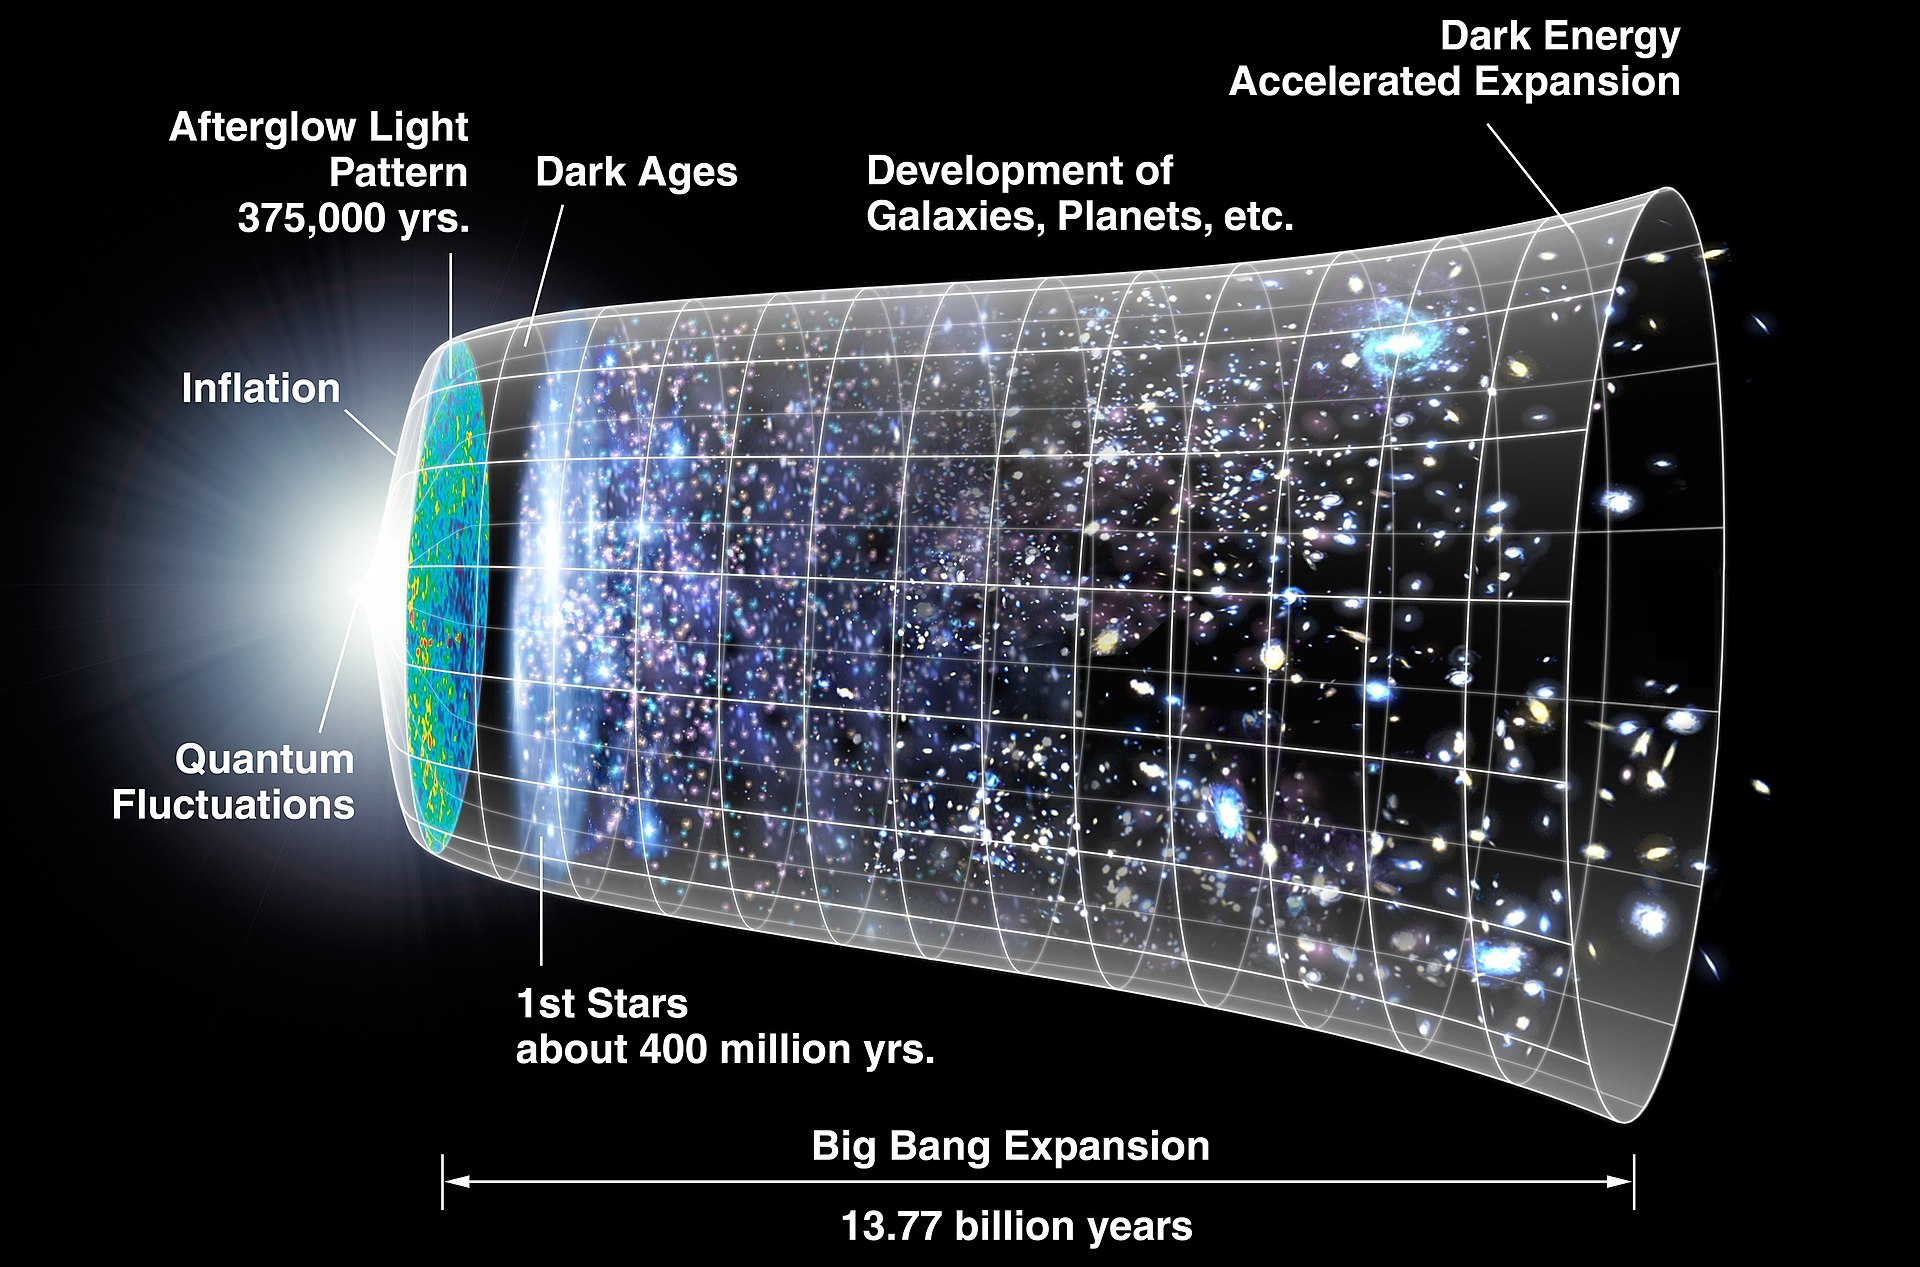
\includegraphics[width=.9\linewidth]{Imagens/CMB_Timeline300_no_WMAP.jpg}
    \caption{A representation of the time evolution of the Universe, starting from the left (the Big Bang) with time passing towards the right. The radius of each section indicates the size of the Universe at that time; during inflation this radius increases very rapidly, indicating an accelerated expansion during this period, while closer to the present the slope of increase in size shows a slight acceleration, indicating the current dark energy accelerated period. Briefly after the inflation period (in cosmological time), the photons decouple from baryons, leaving a radiation field in the Universe, resulting in the CMB, represented in the image by the afterglow of inflation. After this, the only radiation in the Universe is this afterglow for many years, during that time structure starts to form from the small inhomogeneities left by quantum fluctuations in the very early stages of the Universe, forming the first stars and then the first galaxies. Credit: \href{https://map.gsfc.nasa.gov/media/060915/index.html}{NASA/WMAP Science Team}.}
    \label{fig:cosmo_brief_history}
\end{figure}

\section{Inhomogeneities and Anisotropies}

The existence of structures -- nebulae, stars, galaxies, clusters -- in the Universe indicates that, throughout its history, it has been inhomogeneous and anisotropic at some scale. These perturbations to the uniform background are relatively small though, take the CMB for instance: CMB anisotropies are around 5 orders of magnitude lower than its average blackbody temperature \cite{WMAP_results}. 

In this scenario, there is no known theoretical model that can predict the exact behavior of every particle in the Universe. Therefore, we turn to a statistical prediction taking into account the properties of space-time and the components of the Universe. In this section, the first order equations that govern these properties will be shown by introducing perturbations both to the metric and to the stress-energy tensor. 

\subsection{Perturbed Space-Time}

In the $\Lambda$CDM model, to account for perturbations in the uniform background previously set, we work in the Newtonian gauge, which leads to the following form for the metric:

\begin{equation}\label{eq:tensor_perturbations}
\begin{cases}
    g_{00}=-1-2\Psi(\mathbf{x},t),\\
    g_{0i}=g_{i0}=0,\\
    g_{ij}=a^2(t)\delta_{ij}[1+2\Phi(\mathbf{x}, t)].
\end{cases}
\end{equation}

In equation \eqref{eq:tensor_perturbations}, $\Psi$ corresponds to the Newtonian potential and governs the movement of nonrelativistic objects \cite{dodelson2020modern}, while $\Phi$ is a perturbation to the spatial curvature.

With the use of the geodesic equation on this new tensor and using a first order approximation, it is possible to obtain the following results for the equations of motion of particles traveling through the perturbed space-time:

\begin{equation}\label{ch2:dxidt}
    \dv{x^i}{t}=\frac{\hat{p}_i}{a}\frac{p}{E}(1-\Phi+\Psi),
\end{equation}
\begin{equation}\label{ch2:dpidt}
    \dv{p^i}{t}=-(H+\dot{\Phi})p^i-\frac{E}{a}\partial_i\Psi-\frac{1}{a}\dv{p^i}{E}p^k\partial_k\Phi+\frac{p^2}{aE}\partial_i\Phi.
\end{equation}

We can use

\begin{equation}
    \dv{p}{t}=\dv{}{t}\sqrt{\delta_{ij}p^i p^j}=\delta_{ij}\frac{p^i}{p}\dv{p^j}{t}
\end{equation}

\noindent and $\hat{p}^i=p^i/p$ in combination with equation \eqref{ch2:dpidt} to find separate equations for $p$ and $\hat{p}^i$:

\begin{equation}\label{ch2:dpdt}
    \dv{p}{t}=-[H+\dot{\Phi}]p-\frac{E}{a}\hat{p}^i\partial_i\Psi,
\end{equation}
\begin{equation}\label{ch2:dp_hati_dt}
    \dv{\hat{p}^i}{t}=\frac{E}{ap}[\delta^{ik}-\hat{p}^i\hat{p}^k]\partial_k\left(\frac{p^2}{E^2}\Phi-\Psi\right).
\end{equation}

As for the dynamics of the field perturbations, it is possible to use Einstein's field equations to obtain, in Fourier space, the equations for scalar perturbations on the gravitational potentials \cite{dodelson2020modern}

\begin{equation}\label{ch2:first_dynamic_equation}
    k^2\Phi+3H(\dot{\Phi}-H\Psi)=-4\pi Ga^2(\rho_{DM}\delta_{DM}+\rho_b\delta_b+4\rho_\gamma \Theta_0+4\rho_\nu \mathcal{N}_0),
\end{equation}
\begin{equation}\label{ch2:second_dynamic_equation}
    k^2(\Phi+\Psi)=-32\pi Ga^2(\rho_\gamma \Theta_2+\rho_\nu \mathcal{N}_2).
\end{equation}

Here, $\rho$ indicates the average density of a component, $\delta$ represents the perturbation to these densities relative to the average (also known as the matter contrast), and the indexes $DM$, $b$, $\gamma$ and $\nu$ indicate the quantities related to dark matter, baryons, radiation and neutrinos respectively. The terms $\Theta_0$, $\Theta_2$, $\mathcal{N}_0$ and $\mathcal{N}_2$ are obtained in the calculation of the perturbed energy-momentum tensor, they are defined as

\begin{equation}\label{ch2:Fl}
    F_\ell=\frac{1}{(-i)^\ell}\int_{-1}^1 \frac{\mathcal{P}_\ell(\mu)F(\mu)}{2}d\mu,
\end{equation}

\noindent where $F$ can either represent $\Theta$ or $\mathcal{N}$; $\mu=\hat{k}\cdot \hat{p}$ is the cosine between the momentum direction of the photon and the Fourier space wavevector; $P_\ell$ are Legendre polynomials; the functions $\Theta(\mu)$ and $\mathcal{N}(\mu)$ are dimensionless fields that quantify the perturbations of photon and neutrino distributions with respect to the homogeneous background; and $i$ is the imaginary unit $i^2=-1$. 

\subsection{The Boltzmann Equation}

The Boltzmann equation is a fundamental component in the study of every component of the Universe. One general form of writing the Boltzmann equation is

\begin{equation}\label{ch2:Boltzmann_general}
    \dv{f}{t}=\pdv{f}{t}+\pdv{f}{x^i}\cdot \dv{x^i}{t}+\pdv{f}{p}\dv{p}{t}+\pdv{f}{\hat{p}^i}\cdot \dv{\hat{p}^i}{t}=C[f],
\end{equation}

\noindent where $f$ is the distribution function of the component to be analyzed and $C[f]$ is the collision term, a factor that is calculated by considering the interactions of such components.

Using formulas \eqref{ch2:dpdt} and \eqref{ch2:dp_hati_dt} with the Boltzmann equation and assuming $E=p$, i.e. assuming a relativistic particle, the full first order Boltzmann equation for photons is

\begin{equation}\label{ch2:full_photon_boltzmann_eq}
\begin{split}
    \dv{f}{t}=&\pdv{f}{t}+\pdv{f}{x^i}\frac{\hat{p}^i}{a}(1-\Phi-\Psi)-\pdv{f}{p}\left\{[H+\dot{\Phi}]p +\frac{1}{a}p^i\partial_i\Psi\right\}\\
    &+\pdv{f}{\hat{p}^i}\frac{1}{a}\left[\partial_i(\Phi-\Psi)-\hat{p}^i\hat{-}^k\partial_k(\Phi-\Psi)\right].
\end{split}
\end{equation}

The first order approximation is being used, and so it is possible to simplify this expression further. For instance, the distribution $f$ for the homogeneous background takes the form of Bose-Einstein's distribution, which means there is no dependence on $\hat{p}^i$ and $x^i$ in this case. It is commonly assumed that the deviations from this distribution are of the same order of the perturbations $\Phi$ and $\Psi$, so both $\pdv{f}{x^i}$ and $\pdv{f}{\hat{p}^i}$ are first order factors, multiplied by $\Phi$ or $\Psi$ result in second order terms which can be neglected, resulting in

\begin{equation}\label{ch2:Boltzmann_photon_final}
    \dv{f}{t}=\pdv{f}{t}+\frac{\hat{p}^i}{a}\pdv{f}{x^i}-\left[H+\dot{\Phi}+\frac{1}{a}\hat{p}^i\partial_i\Psi\right]p\pdv{f}{p}.
\end{equation}

This is an important equation for the understanding of the CMB, but the description of anisotropies for massive particles is still important, for which the same assumptions are made, resulting in 

\begin{equation}\label{ch2:Boltzmann_matter_final}
    \dv{f}{t}=\pdv{f}{t}+\frac{p}{Ea}\hat{p}^i\pdv{f}{x^i}-\left[H+\dot{\Phi}+\frac{E}{ap}\hat{p}^i\partial_i\Psi\right]p\pdv{f}{p}.
\end{equation}

The only difference between these equations is the term $E/p$ which, in the case of radiation, is equal to 1. The first order approximation for non-relativistic matter breaks down in the late Universe, a non-linear model is necessary in this scenario. 

To arrive at a differential equation, a function to describe the perturbations needs to be defined, and so does the distribution function. Taking the CMB as an example, the perturbed form of the temperature distribution for CMB photons in general can be defined as

\begin{equation}\label{T(x,p,t)}
    T(\mathbf{x}, \hat{\mathbf{p}}, t)=\bar{T}(t)[1+\Theta(\mathbf{x}, \hat{\mathbf{p}}, t)],
\end{equation}

\noindent where $\bar{T}$ is the average temperature in a given time and $\Theta$ is the same field presented in equation \eqref{ch2:Fl}, that quantifies the perturbations of the CMB distribution with respect to its average value. This perturbation field can be expressed in terms of the set of functions $\Theta_\ell$ defined in \eqref{ch2:Fl} by the following equation in Fourier space:

\begin{equation}\label{Theta_&_Thetal}
    \Theta(\hat{\mathbf{k}}, \mu)=\sum_{\ell=0}^\infty (2\ell+1)(-i)^\ell \Theta_\ell(\hat{\mathbf{k}}) \mathcal{P}_\ell(\mu).
\end{equation}

If we use the Bose-Einstein distribution for the temperature defined in \eqref{T(x,p,t)} and expand it to its first order, we obtain 

\begin{equation}\label{f(x,p,t)_first_order}
    f(\mathbf{x}, \mathbf{p}, t)=f^{(0)}(p,t)-p\pdv{f^{(0)}(p,t)}{p}\Theta(\mathbf{x}, \mathbf{p}, t),
\end{equation}

\noindent where

\begin{equation}\label{f(0)}
    f^{(0)}(p,t)=\left[\text{exp}\left(\frac{p}{\Bar{T}}\right)-1\right]^{-1}
\end{equation}

We can then expand the Boltzmann equation using the results in \eqref{f(x,p,t)_first_order} and \eqref{f(0)} and take into account Compton scattering to calculate the collision term $C[f]$ to obtain a differential equation for the CMB photons. We can use similar procedures, using adequate distribution functions, and obtain a set of coupled differential equations to describe the evolution of the perturbations of every known component of the Universe in Fourier space \cite{dodelson2020modern}:

\begin{equation}\label{diff_eq_radiation_perturbs}
    \dot{\Theta}+\frac{ik\mu}{a}(\Theta+\Psi)=-\dot{\Phi}-\dot{\tau}\left[\Theta_0-\Theta+\mu v_b-\frac{1}{2}\mathcal{P}_2(\mu)(\Theta_2+\Theta_{P2}+\Theta_{P0})\right],
\end{equation}
%\begin{equation}
%    \dot{\Theta}_P+ik\mu\Theta_P=-\dot{\tau}\left\{-\Theta_P+\frac{1}{2}[1-\mathcal{P}_2(\mu)](\Theta_2+\Theta_{P2}+\Theta_{P0})\right\},
%\end{equation}
\begin{equation}
    \dot{\delta_c}+\frac{ik}{a}v_c=-3\dot{\Phi},
\end{equation}
\begin{equation}
    \dot{\delta_b}+\frac{ik}{a}v_b=-3\dot{\Phi},
\end{equation}
\begin{equation}
    \dot{v_c}+\frac{H}{a}v_c=-\frac{ik}{a}\Psi,
\end{equation}
\begin{equation}
    \dot{v_b}+\frac{H}{a}v_b=-\frac{ik}{a}\Psi+\frac{4\rho_\gamma}{3\rho_b}\dot{\tau}(v_b+3i\Theta_1),
\end{equation}
\begin{equation}\label{diff_eqs:neutrino_perturbations}
    \dot{\mathcal{N}}+\frac{ik\mu}{a}\mathcal{N}=-\dot{\Phi}-\frac{ik\mu}{a}\Psi.
\end{equation}

Here, $\Theta_{P\ell}$ is defined by equation \eqref{ch2:Boltzmann_general} using $F=\Theta_P$, where $\Theta_P$ is the polarization field; $\delta$ and $\delta_b$ are the perturbations to the matter and baryon distributions respectively; $v$ and $v_b$ are the bulk velocities of the fluids in the stress-energy tensor for matter and baryons respectively; $\rho_b$ and $\rho_\gamma$ are the baryon and radiation energy densities respectively; and $\tau$ is the optical depth to recombination, which in this context measures the transparency of the Universe at a certain redshift $z$:	

\begin{equation}\label{def:optical_depth}
	\tau(z)=\int_0^z \frac{\sigma_T n_e(z')}{H(z')} dz',
\end{equation}

\noindent where $\sigma_T$ is the Thomson scattering cross-section and $n_e$ is the number density of free electrons in the Universe at redshift $z'$.

These equations, alongside equations \eqref{ch2:first_dynamic_equation} and \eqref{ch2:second_dynamic_equation}, are very complex to be solved analytically, so it is common to evolve them numerically, and there are a few codes developed specifically for this purpose. One of them, that has been used in this project, is CAMB \cite{CAMB:Lewis1999bs, CAMB:Lewis2002ah}.

\section{The Cosmic Microwave Background}

With the dynamical equations for photons determined, one can obtain the temperature perturbation distribution $\Theta$ if initial conditions are provided. With the equations already presented, it is possible to show that the initial conditions at the early Universe depend only on the initial conditions for $\Phi$ \cite{dodelson2020modern}, which are then evolved through the inflationary period assuming the existence of a quantum scalar field $\phi(\mathbf{x}, t)$ that drives a brief accelerated expansion. 

At the end of inflation, the energy of the scalar quantum field (the inflaton) is transfered to standard model particles and possibly to dark matter. Eventually baryons form from standard model quarks and gluons and together with electrons and photons form the so called photon-baryon fluid, that can be described by the differential equations \eqref{diff_eq_radiation_perturbs} - \eqref{diff_eqs:neutrino_perturbations}. The initial distribution obtained for this fluid can then be evolved to predict the present anisotropies to the uniform background. %To analyze these predictions, the statistical behavior of each component of the Universe is taken: either their spectral densities -- usually called their power spectra -- or what is known as their correlation spectra. 

\subsection{CMB Autocorrelation Spectrum}

Equation \eqref{T(x,p,t)} explicitly assumes a dependence in position, time, and momentum direction. Measurements made on Earth can assume a fixed value for time since our measurements are taken in a period negligible in the cosmological scale, but the translational movement of the Earth is relevant to our measurements: measurements of the CMB made by a non-comoving observer, when projected onto a sphere, lead to a strong dipole pattern in the temperature distribution, modulation of the multipole terms and relativistic aberration at angular scales of a few arcminutes \cite{COBE_calibration, Planck_doppler, esteban_msc}.

Despite these effects, measurements of the temperature distribution can be projected onto a sphere, making it possible to describe this distribution simply using two angle variables, or simply $\hat{\mathbf{p}}$.

We can expand the temperature perturbations in spherical harmonics:

\begin{equation}\label{ch2:Theta_spherical harmonics}
    \Theta(\mathbf{x}, \hat{\mathbf{p}}, t)=\sum_{\ell=1}^\infty \sum_{m=-\ell}^\ell a_{\ell m}(\mathbf{x}, t)Y_{\ell m}(\hat{\mathbf{p}}).
\end{equation}

All the information about temperature maps of the CMB measured on Earth are contained in the set of $a_{\ell m}$ values. Given the limited number of pixels $N_\text{pix}$ of any of these maps, there is a maximum value of $\ell$ ($\ell_\text{max}$) up to which statistically meaningful information can be retrieved. For each value of $\ell$, there are $2\ell+1$ values of $m$ -- and $a_{\ell m}$ -- in the series. %, a hypothetical observed map with precision $p_r$ in squared radians would have $4\pi/p_r$ pixels, setting this number of pixels equal to the number of $a_{\ell m}$ used to describe this map gives a reasonable estimation of $\ell_\text{max}$ \cite{dodelson2020modern}, so %a specific example of this is in page 252 of the 2020 edition of Dodelson, I just generalized it in terms of a general precision p_r instead of using the example's p_r=7º.

%\begin{equation}\label{Npix}
%    \sum_{\ell=0}^{\ell=\ell_\text{max}}(2\ell+1)=(\ell_\text{max}+1)^2=N_\text{pix}=\frac{4\pi}{p_r}.
%\end{equation}

Using the orthogonality property of the spherical harmonics, one can obtain a direct expression for $a_{\ell m}$ in terms of the angular distribution of the perturbations:

\begin{equation}\label{ch2:alm=int...}
    a_{\ell m}(\mathbf{x}, t)=\int \frac{d^3k}{(2\pi)^3}e^{i\mathbf{k}\cdot\mathbf{x}}\int d\Omega Y_{\ell m}^*(\hat{\mathbf{p}})\Theta(\mathbf{k}, \hat{\mathbf{p}}, t).
\end{equation}

There are available codes that efficiently and precisely calculate $a_{\ell m}$ from a pixelized map and vice versa, the one used in this work was HEALPix \cite{Healpix}. Under the hypothesis that the spherical harmonics coefficients $a_{\ell m}$ are independent Gaussian random variables with zero mean, all its statistical properties are contained in the variance $C_\ell$, also known as the power spectrum:

\begin{equation}\label{def:autocorrelation}
    \av{a_{\ell m} a^*_{\ell' m'}}=\delta_{\ell\ell'}\delta_{mm'}C(\ell),
\end{equation}

\noindent where $\delta_{mm'}$ is the Kronecker delta taking $m$ and $m'$ as arguments.

The fact that for lower values of $\ell$ there are fewer coefficients $a_{\ell m}$ naturally leads to lower multipoles $\ell$ having higher uncertainty, this property is usually called cosmic variance and can be expressed using \cite{dodelson2020modern} 

\begin{equation}\label{cosmic_variance}
    \left(\frac{\Delta C(\ell)}{C(\ell)}\right)_\text{cosmic variance}=\sqrt{\frac{2}{2\ell+1}}.
\end{equation}

The temperature autocorrelation defined in equation \eqref{def:autocorrelation} is usually expressed as $C_\ell^{TT}$, but sometimes a modified spectrum $D_\ell^{TT}=\frac{\ell(\ell+1)}{2\pi}C_\ell^{TT}$ is used for visualization purposes. Figure \ref{fig:Planck_spectrum} shows Planck's CMB power spectrum data and its corresponding best-fit spectrum assuming a $\Lambda$CDM cosmology.

\begin{figure}[!htb]
    \centering
    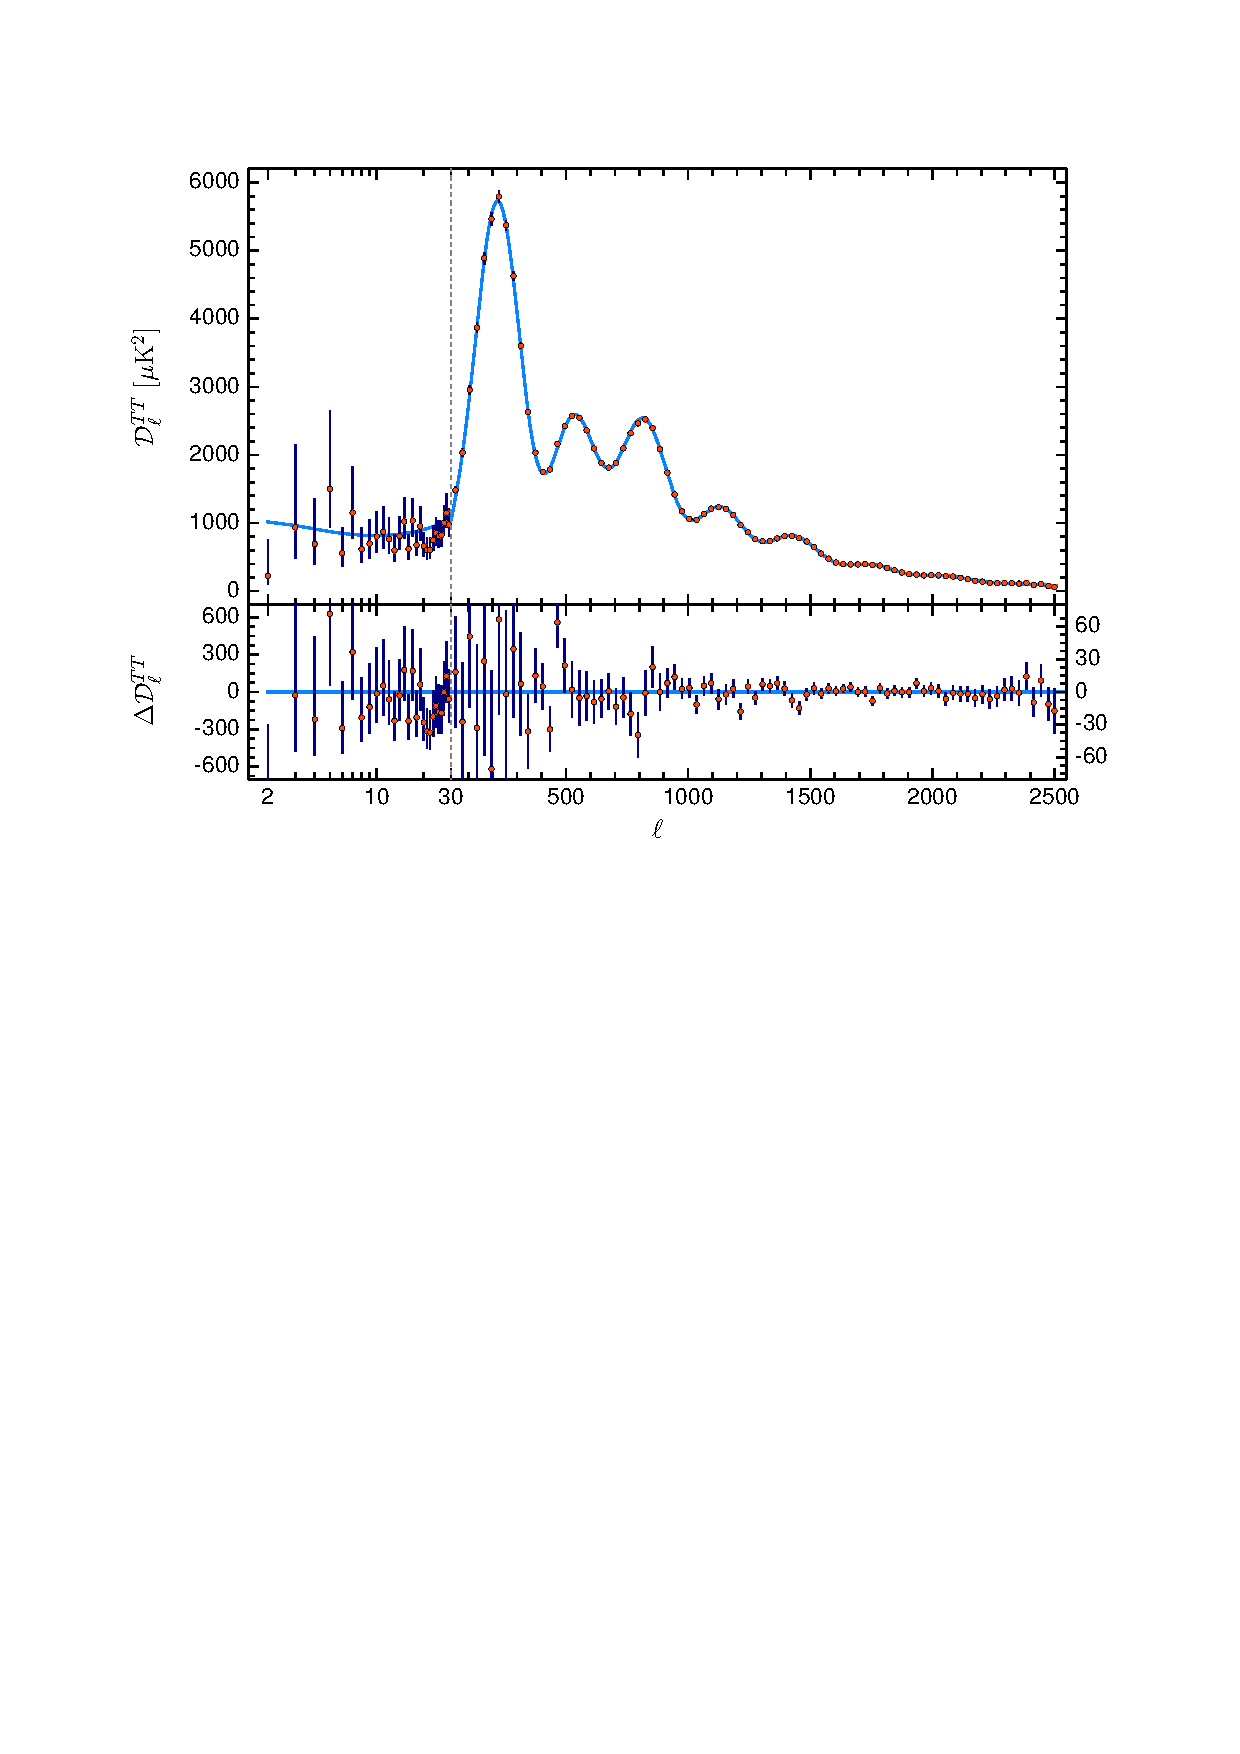
\includegraphics[width=.9\linewidth]{Imagens/planck_spectrum.pdf}
    \caption{Planck 2018 CMB temperature power spectrum: the blue line corresponds to a $\Lambda$CDM cosmology best-fit to the data points in orange. For $\ell<30$ a logarithmic scale was used and the data points correspond to the $D_\ell^{TT}$ for each value of $\ell$, while for $\ell\ge 30$ a linear scale was used and the data points correspond to binned values for the data for $D_{\ell}^{TT}$. The error bars show $\pm 1\sigma$ uncertainties, including cosmic variance. Extracted from \cite{Planck_results}.}
    \label{fig:Planck_spectrum}
\end{figure} 

Table \ref{tab:planck_parameters} summarizes the values of the best-fit parameters corresponding to the blue line of Figure \ref{fig:Planck_spectrum} and were extracted from reference \cite{Planck_results}. The model is based on 6 basis parameters as can be seen in the upper part of table 2.2 and are related to the baryonic ($\Omega_b h^2$) and cold dark matter fractional densities scaled by $h^2$, the sound horizon angular scale at recombination ($\Theta_{MC}$), the optical depth up to the last scattering surface  due to reionization ($\tau$), the normalization of the primordial spectral of scalar perturbations during inflation ($A_s$) and its spectral index ($n_s$). The last three parameters are dubbed derived because they can be inferred from the 6 basis ones.

\begin{table}[!htb]
    \centering
    \begin{tabular}{cc} \hline
     Parameter & Best-fit \\ \hline
     $\Omega_b h^2$ & $0.02237\pm 0.00015$\\
     $\Omega_c h^2$ & $0.1200\pm 0.0012$\\
     $100\Theta_{MC}$ & $1.04092\pm 0.00031$ \\
     $\tau$ & $0.0544\pm 0.0073$\\ 
     $\ln{(10^{10}A_s)}$ & $3.044 \pm 0.014$ \\ 
     $n_s$ & $0.9649 \pm 0.042$ \\ \hline
     %$\Omega_k$ & $0.0$ \\ \hline
     $\Omega_m$ & $0.3153 \pm 0.0073$ \\
     $H_0$ & $67.36 \pm 0.54$ km/s/Mpc \\
     $\sigma_8$ & $0.8111 \pm 0.0060$ \\ \hline
    \end{tabular}
    \caption{Best fit values of cosmological parameters reported by the Planck collaboration using a combined likelihood with temperature and polarization spectra and lensing data. Here $h=H_0/(100\text{ km/s/Mpc})$ is the reduced Hubble constant, $\Theta_{MC}$ is the angular scale of the sound horizon at the surface of last scattering, $A_s$ is the amplitude of the primordial scalar perturbations, $n_s$ is the spectral index of the primordial scale perturbations, $\Omega_m=\Omega_c+\Omega_b$ is the matter energy density and $\sigma_8$ measures the amplitude of density fluctuations at the scale of $8h^{-1}$ Mpc. The first 6 parameters are used for solving the perturbation equations with CAMB and the last 3 are derived from the solution.}
    \label{tab:planck_parameters}
\end{table}

The best fit values shown in Tables \ref{tab:rhos&Omegas} and \ref{tab:planck_parameters} are the values that have been used in this project for the fiducial $\Lambda$CDM model, with $\Omega_k=0$ being used, justifying the assumption of a flat metric.

\subsection{The Hubble Tension}

There are multiple ways to estimate the Hubble constant $H_0$, we have discussed its determination through a heavily model-dependent technique, which is by sampling its best-fit value by comparing the $\Lambda$CDM model's prediction of the CMB temperature power spectrum with CMB data. Planck's results using this technique have been showing a tension with a more direct technique, that relies on the so-called cosmic distance ladder to construct a relation of distance modulus $\mu_0$ of astronomical objects and redshift $z$ and determine $H_0$ from these datasets \cite{Riess2021}. The method uses different astronomical objects in different redshift intervals, thus needing different techniques and callibrations, data at lower redshift ranges (or rungs) are used to callibrate the following rung.

The value obtained using this method in \cite{Riess2021} is $H_0=(73.04\pm 1.01) \text{km}\text{s}^{-1} \text{Mpc}^{-1}$, which consists of a $5\sigma$ difference compared with Planck's estimate shown in Table \ref{tab:planck_parameters}, showing a tension between the two results.

Currently, there is a significant number of studies trying to understand this tension, with some papers studying the possibility of systematic effects being responsible for it \cite{systematics2023,alexandra_msc}, while other papers explore adjustments to the $\Lambda$CDM model\cite{growth_constraint}, mostly in regards to the description of dark energy, which will be discussed in a section \ref{sect:dark_energy}.

\subsection{Analytical Approximation}

Although solving equations such as \eqref{diff_eq_radiation_perturbs} numerically gives accurate results, obtaining an analytical approximation to these equations helps us understand the underlying physical effects that most influence the evolution of the perturbations. Working on the tightly coupled limit and assuming recombination to be an instantaneous process happening at conformal time $\eta=\eta_*$, one can obtain the following equation for the CMB temperature fluctuation multipoles in Fourier space \cite{dodelson2020modern}:

\begin{equation}\label{ch2:Thetal_approx}
\begin{split}
    \Theta_\ell(k,\eta_0)\approx &[\Theta_0(k,\eta_*)+\Psi(k,\eta_*)]j_\ell[k(\eta_0-\eta_*)]\\
    &+iv_b(k,\eta_*)\left\{j_\ell[k(\eta_0-\eta_*)]-(l+1)\frac{j_\ell[k(\eta_0-\eta_*)]}{k(\eta_0-\eta_*)}\right\}\\
    &+\int_0^{\eta_0} d\eta e^{-\tau}[\Psi'(k,\eta)-\Phi'(k,\eta)]j_\ell[k(\eta_0-\eta)],
\end{split}
\end{equation}

\noindent where $j_\ell$ are spherical Bessel functions, the conformal time $\eta$ is defined as

\begin{equation}\label{def:conformal_time}
    \eta=\int_0^t \frac{dt}{a(t)},
\end{equation}

\noindent and $\eta_*$ is the value of $\eta$ that maximizes the visibility function $g(\eta)$:

\begin{equation}\label{def:visibility_function}
    g(\eta)=-\tau'e^{-\tau}.
\end{equation}

With these conventions, the derivative with respect to $\eta$ is being represented by the prime notation, while the dot notation used in equation \eqref{diff_eq_radiation_perturbs} will still indicate derivatives with respect to time.

There are three main contributors to the solution \eqref{ch2:Thetal_approx}:

\begin{itemize}
    \item The $(\Theta_0+\Psi)$ term is usually called the Sachs-Wolfe term, which is associated with Baryon Acoustic Oscillations (BAO), which are fluctuations in the density of the visible baryonic matter of the Universe, caused by acoustic density waves in the primordial plasma of the early Universe \cite{dodelson2020modern};
    \item The $iv_b$ term shows a contribution to the spectrum related to a Doppler shift of the BAO, due to its dependence on a non-zero bulk velocity of the baryons during recombination;
    \item The last term, an integral involving the time variations of the gravitational potentials, represents the Integrated Sachs-Wolfe (ISW) effect. Its dependence on the on the derivative with respect to conformal time of the gravitational potential makes it so that it only has a non-negligible effect on the CMB at cosmological periods with significant time variability of these potentials: At around $a\sim 10^{-4}$ the Universe transitioned from a radiation-dominated to a matter-dominated Universe (early ISW), and recently -- around $a\sim 0.6$\cite{dark_energy_era} according to the $\Lambda$CDM model -- the Universe transitioned from a matter-dominated Universe to the current dark energy dominated Universe (late ISW). 
\end{itemize}

Figure \ref{fig:CMB_contributions} shows how these terms contribute to the full CMB temperature autocorrelation power spectrum. It shows the relevance of the late-ISW contribution in lower multipoles, as well as the strong influence of the Sachs-Wolfe term with the accoustic peaks of the spectrum and the phase shift of the Doppler term's contribution compared to the Sachs-Wolfe one.

\begin{figure}[!htb]
	\centering
	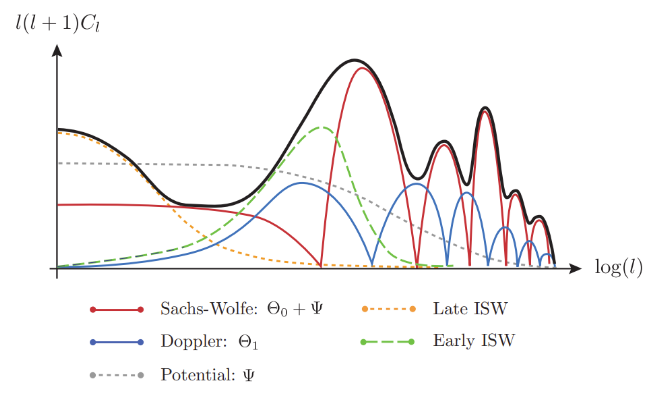
\includegraphics[width=.75\linewidth]{Imagens/CMB_contributions.png}
	\caption{Main contributions for the temperature power spectra from the Sachs-Wolfe effect (SW: red), Integrated Sachs-Wolfe effect (ISW: green and orange), Doppler effect (blue) and pure gravitational contribution (gray).}
	\label{fig:CMB_contributions}
\end{figure}

\section{The Integrated Sachs Wolfe Effect}\label{ch2:ISW_effect_section}

It was proposed that the cross-correlation spectrum between CMB maps and matter contrast could be used to detect the ISW effect \cite{Turok96}, and since then many works have reported the detection of this signal \cite{cross_corr:Afshordi, cross_corr:Crittenden2005a, cross_corr:Crittenden2005b, cross_corr:Planck}. In this section, a framework for theoretical estimations of the ISW contribution to this cross-correlation will be discussed.

\subsection{The Matter Power Spectrum}

While the CMB is usually described as a 2-dimensional map, the matter distribution in the Universe is characterized by their 3-dimensonal spatial coordinates measured with respect to the solar system position, therefore, three coordinates are necessary from which 2D projections can be made for different redshift shells. Again using Fourier space, we first define the 3D power spectrum for the distribution of matter perturbations in the Universe $P(k)$ as

\begin{equation}\label{def:P(k)}
    \av{\delta(\mathbf{k}, z) \delta^*(\mathbf{k}', z)}=(2\pi)^3 P(k,z) \delta_D(\mathbf{k}-\mathbf{k}'),
\end{equation}

\noindent where $\delta_D$ is the Dirac delta, $\delta$ is the previously shown matter perturbation distribution in the Universe and the $*$ superscript indicates the complex conjugate of a quantity. Again, using appropriate initial conditions, one can theoretically predict $\delta(\mathbf{k})$ and thus $P(k,z)$ using CAMB. Figure \ref{fig:matter_PS} shows the results for this calculation.  

\begin{figure}[!htb]
    \centering
    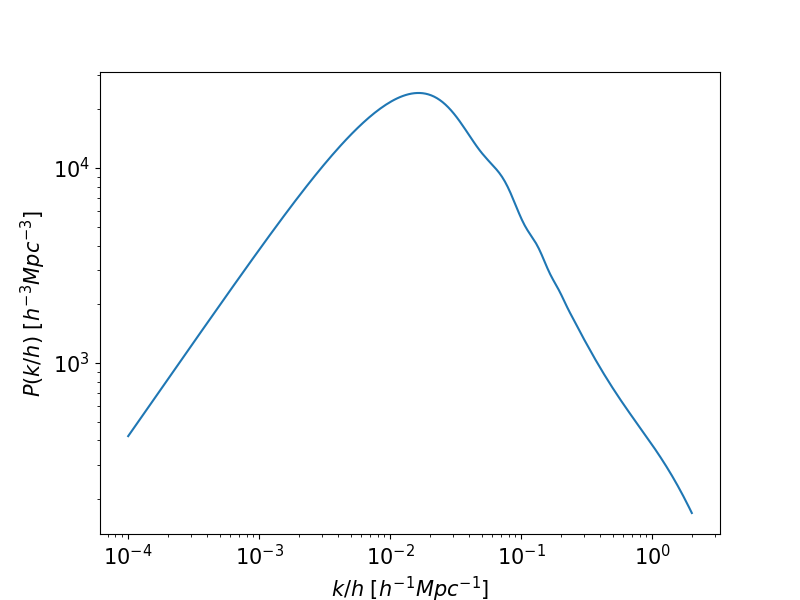
\includegraphics[width=.75\linewidth]{Imagens/Pk_3dmatter_LCDM.png}
    \caption{Matter power spectrum calculated as a function of $k/h$, where $h$ is the already defined reduced Hubble constant, using both a linear approximation and the so-called HALOFIT model \cite{Halofit2020} with cosmological parameters according to our fiducial $\Lambda$CDM model.}
    \label{fig:matter_PS}
\end{figure}

The HALOFIT model is a semi-analytical method to determine a non-linear solution for $P(k,z)$, it is based in the Halo Model, which assumes that at small scales, the evolution of structures can be described by gravitational collapse to spherically symmetric halos whose evolution posterior to their formation decouple from the background cosmology. The corrections due to the HALOFIT model are not relevant in large scales, as shown in Figure \ref{fig:matter_PS}, in which both spectra are indistinguishable at low values of $k$, only at higher values of k -- small scales -- the two spectra clearly diverge. In terms of the correlation power spectra, one can already notice a significant difference in the predicted spectra at around $\ell=40$ \cite{Moura-Santos_2016}, showing very clearly the importance of using HALOFIT for our analysis.

It is important to highlight that HALOFIT is only valid assuming an equation of state parameter of $w=-1$ to dark energy. For more general scenarios one can use, for instance, the more modern HMcode \cite{HMcode}.

\subsection{The Galaxy-CMB Correlation Spectra}\label{ch2:correlations}

To obtain the autocorrelation for a projection of a matter density distribution on a spherical shell on a certain redshift $z$, one has to choose a way to trace the matter density with an observable. The observable used in this work is the so called galaxy contrast map: by measuring galaxy densities $\rho_g(\mathbf{k})$ covering the sky and taking the average galaxy density over the entire sky $\bar{\rho}_g$, the galaxy contrast map can be calculated as

\begin{equation}\label{def:contrast_map}
	\delta_g(\mathbf{k})=\frac{\rho_g(\mathbf{k})-\bar{\rho}_g}{\bar{\rho}_g}.
\end{equation}

It is common to assume that the galaxy contrast map takes the form $\delta_g=b_g\delta$ where $b_g$ is called the bias factor, which will be treated here as a slowly varying function of redshift and will assume slightly different values depending on the peak redshift of the selected galaxies. From this point, the same process needed to calculate \eqref{def:autocorrelation} can be applied: Expand the distribution in spherical harmonics with factors $a_{\ell m}^g$ and calculate the variance of these variables to obtain an autocorrelation spectrum $C^{gg}(\ell)$.

Similarly, instead of calculating an autocorrelation spectrum, one can calculate a cross-correlation between two perturbation distributions, which is analogous to definition \eqref{def:autocorrelation}:

\begin{equation}\label{av(ag, at)}
    \av{a_{\ell m}^ta_{\ell' m'}^g}=C^{tg}_\ell\delta_{\ell \ell'}\delta_{mm'}.
\end{equation}

By using equation \eqref{ch2:Theta_spherical harmonics} one can express $a_{\ell m}$ in terms of $\Theta_\ell$, which can be expanded using equation \eqref{ch2:Thetal_approx}, this expansion and the correlation definitions allow us to find analytical expressions for all correlation functions discussed so far using the approximations discussed, but we can also use the ISW term in equation \eqref{ch2:Thetal_approx} to calculate the its sole contribution to the full correlation spectra. 

Given fields $x$ and $y$, representing either the ISW contribution to the CMB temperature ($x,y=t$) or the galaxy contrast ($x,y=g$), we can calculate the associated auto- or cross-correlation spectra using:

\begin{equation}\label{Cl_direct_calculation}
    C^{xy}_\ell=\frac{2}{\pi}\int dk k^2 W_\ell^x(k)W_\ell^y(k)P(k),
\end{equation}

\noindent where $W_\ell$ are called the kernel functions, which can be calculated using

\begin{equation}\label{Wt}
    W_\ell^t=-3\Omega_m\left(\frac{H_0}{k}\right)^2\int dz \dv{[(1+z)D(z)]}{z} j_\ell[k\chi(z)],
\end{equation}
\begin{equation}\label{Wg}
    W_\ell^g=\int dz b_g(z)\dv{N}{z}D(z)j_\ell[k\chi(z)],
\end{equation}

\noindent where $D(z)$ is the linear growth function (normalized to 1 at $z=0$); $\chi(z)$ is the comoving distance; and $\dv{N}{z}$ is the normalized galaxy redshift distribution, also called the selection function \cite{cross_corr:Afshordi}. A derivation of this equation can be found in Appendix \ref{app:correlations_demo}.

With equation \eqref{Cl_direct_calculation}, we can determine the theoretical spectra for CMB and galaxy autocorrelations and CMB-galaxy cross-correlation directly. Figure \ref{fig:Ctt_ISW_comparison} shows the total CMB autocorrelation and the ISW contribution, both at $z=0$.

\begin{figure}[!htb]
    \centering
    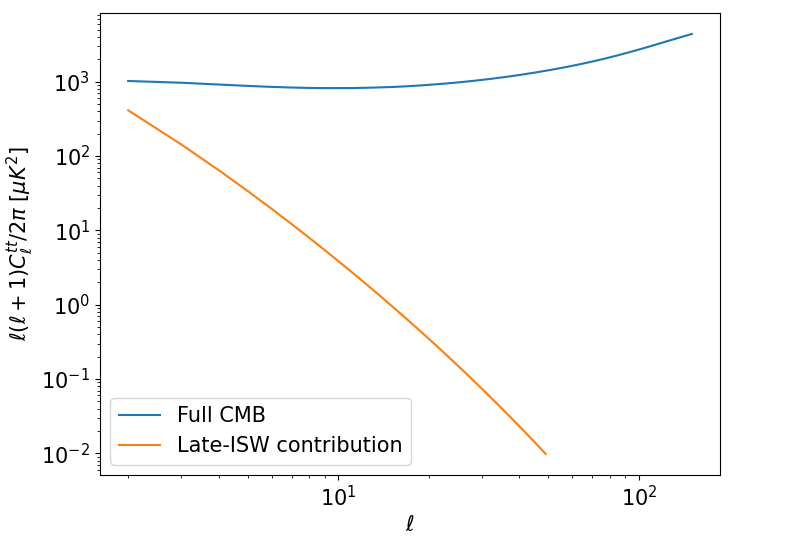
\includegraphics[width=.75\linewidth]{Imagens/Ctt_comparison.png}
	\caption{CMB autocorrelation for the late-ISW term and the full spectrum.The full spectrum was calculated with CAMB and the ISW contribution using a custom designed C++ code. The parameters used are those corresponding to the Planck best fit parameters \cite{Planck_results}.}
    \label{fig:Ctt_ISW_comparison}
\end{figure}

Figure \ref{fig:correlations_theoretical}, on the other hand, shows the galaxy auto-correlation ($C^{gg}$) and the galaxy-CMB cross-correlation ($C^{tg}$) due to ISW as a function of multipole $\ell$.

\begin{figure}[!htb]
	\centering
	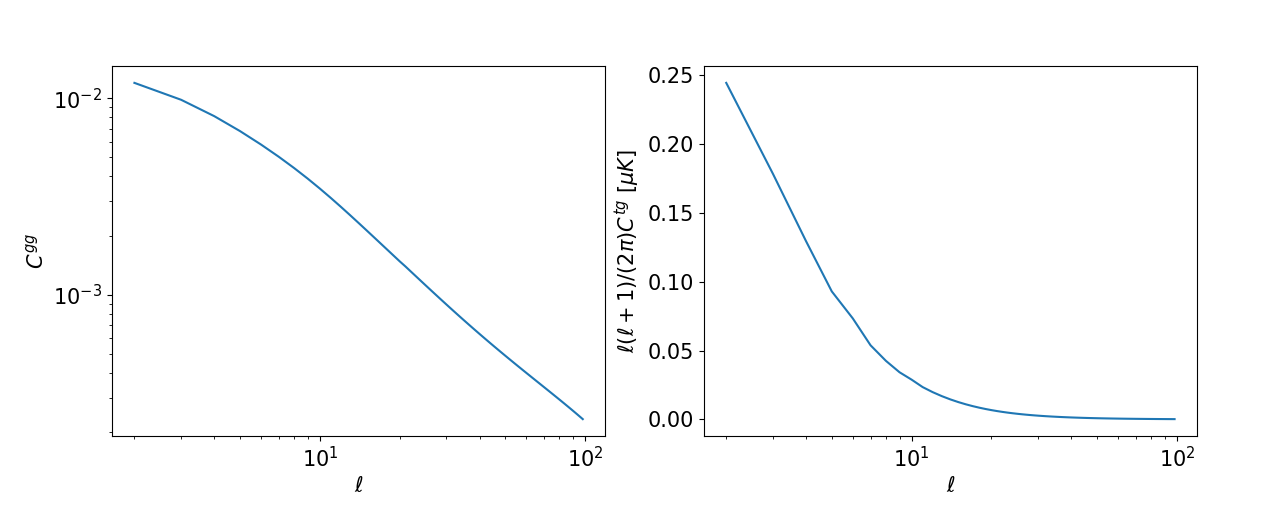
\includegraphics[width=.98\linewidth]{Imagens/Correlations_DoublePlot.png}
	\caption{Galaxy autocorrelation spectrum (left) and late-ISW contribution to the galaxy-CMB cross-correlation (right). The selection function used to calculate these spectra was parametrized to be compatible with 2MASS' galaxy redshift distribution \cite{cross_corr:Afshordi, Moura-Santos_2016}.}
	\label{fig:correlations_theoretical}
\end{figure}

These plots show very clearly that the ISW effect has a lot more relevance in the low multipoles region, where cosmic variance has a significant influence. The selection function is an important aspect of this signal, in chapter \ref{chapter:select_func_optimal} the matter of how to optimize the signal with the use of an idealized selection function will be discussed.

\section{Alternative Dark Energy Models}\label{sect:dark_energy}

Many approaches to study dark energy have been proposed, each of them with different properties, ranging from parameterization of the equation of state \cite{CPL_DE_parametrization, FSLL_DE_parametrization} to alternative fluid models for dark energy \cite{DEDM_fluid, review_DE_ronaldo} and modifications to general relativity \cite{Brane_cosmo_model}. 

A general class of dark energy models are the ones called the k-essence models. The energy-momentum tensor for a k-essence type dark energy is \cite{review_DE_ronaldo}

\begin{equation}\label{k-essence_Tmunu}
´	T_{\mu\nu}=\partial_X \mathcal{L} \nabla_\mu \varphi \nabla_\nu \phi -\mathcal{L} g_{\mu\nu},
\end{equation}

\noindent where $\varphi$ is the k-essence scalar field, $X=-\frac{1}{2}g^{\mu\nu}\partial_\mu \varphi \partial_\nu \varphi$ is a kinetic term and $\mathcal{L}=\mathcal{L}(X, \varphi)$ is the lagrangian density. Equation \eqref{k-essence_Tmunu} can be compared with the perfect fluid equation to obtain

\begin{align}\label{k-essence_results}
	\rho&=2X\partial_X\mathcal{L}-\mathcal{L}, & p&=\mathcal{L}, & c_s^2&=\frac{\partial_X p}{\partial_X \rho},
\end{align}

\noindent where $c_s^2$ is the so-called sound speed of the k-essence fluid, $p$ is the fluid's pressure and $\rho$ its energy density. The value of these parameters influence, for instance, the evolution of the gravitational potentials \cite{DE_variable_soundspeed_Linton2018} and their perturbations -- especially at low values of $c_s$ -- and many other factors that relate to the evolution of the universe, thus having an impact on observables. 

Within k-essence, a very common class of models are the quintessence ones, which are defined by $\mathcal{L}=X-V(\varphi)$, for which we can obtain an equation of state parameter $w=p/\rho$ and sound speed of

\begin{align}\label{quintessence1}
	w&=\frac{X-V}{X+V}, & c_s^2&=1.
\end{align}

In equation \eqref{quintessence1}, $w$ can be time dependent, and its form depends on the form of the potential $V$. Parametrizing this equation as a funtion of redshift and fitting it to the data can be a powerful tool to find what models might better describe dark energy. The simplest parametrization proposed for dark energy's equation of state is called the Chevallier-Polarski-Linder (CPL) parametrization \cite{CPL_DE_parametrization,DE_models}:

\begin{equation}\label{CPL}
    w(z)=w_0+\left(1-\frac{1}{1+z}\right)w_a.
\end{equation}

%One important property of this parametrization and most others is that the value of the equation of state parameter today ($z=0$) is the same as the equation of state parameter of the $\Lambda$CDM model $w_0$

So far, this parametrization has not solved some of the current limitations being faced by the $\Lambda$CDM model, such as the Hubble tension \cite{Hubble_tension_review} and the $\sigma_8$ tension \cite{Planck_results}. It has not improved significantly over the $\Lambda$CDM predictions, but it shows good compatibility with CMB, type IA supernovae and baryon acoustic oscillations (BAO) data \cite{Planck_results}. Planck results using this parametrization are shown in Table \ref{tab:planck_CPL}.

\begin{table}[!htb]
    \centering
    \begin{tabular}{cc} \hline
     Parameter & Marginalized Value \\ \hline
     $w_0$ & $-0.957\pm0.080$\\
     $w_a$ & $-0.29\substack{+0.32 \\ -0.26}$\\
     $H_0 [\text{km s}^{-1}\text{Mpc}^{-1}]$ & $68.31\pm0.82$ \\
     $\sigma_8$ & $0.820\pm 0.011$\\ \hline
     $\Delta \chi^2$ & -1.4 \\ \hline
    \end{tabular}
    \caption{Marginalized values and $68\%$ confidence limits for cosmological parameters, assuming parametrization \eqref{CPL}, obtained by combining Planck temperature and polarization autocorrelation and cross-correlation spectra \cite{Planck_spectra}, type IA supernovae data from the Joint Light Curve Analysis (JLA) \cite{JLA} and BAO data from the Sloan Digital Sky Survey (SDSS) \cite{SDSS}. The $\Delta \chi^2$ value was computed with respect to the $\Lambda$CDM best fits computed from the same data set combination.}
    \label{tab:planck_CPL}
\end{table}

Figure \ref{fig:Dark_energy_tests} shows the influence of different parameter values, using the CPL parametrization, on the CMB temperature autocorrelation spectrum, and compares the expected theoretical spectra with Planck's data. It is important to note that $w_a=1$ is a very extreme scenario, where $w_\text{de}=0$ at very high redshifts, meaning it would behave like matter, which is a behavior very incompatible with the data shown in the plots.

%%% DARK ENERGY IMAGES %%%

\begin{figure}
	\centering
	\makebox[.87\paperwidth]{
	\begin{subfigure}[t]{.43\paperwidth}
		\centering
		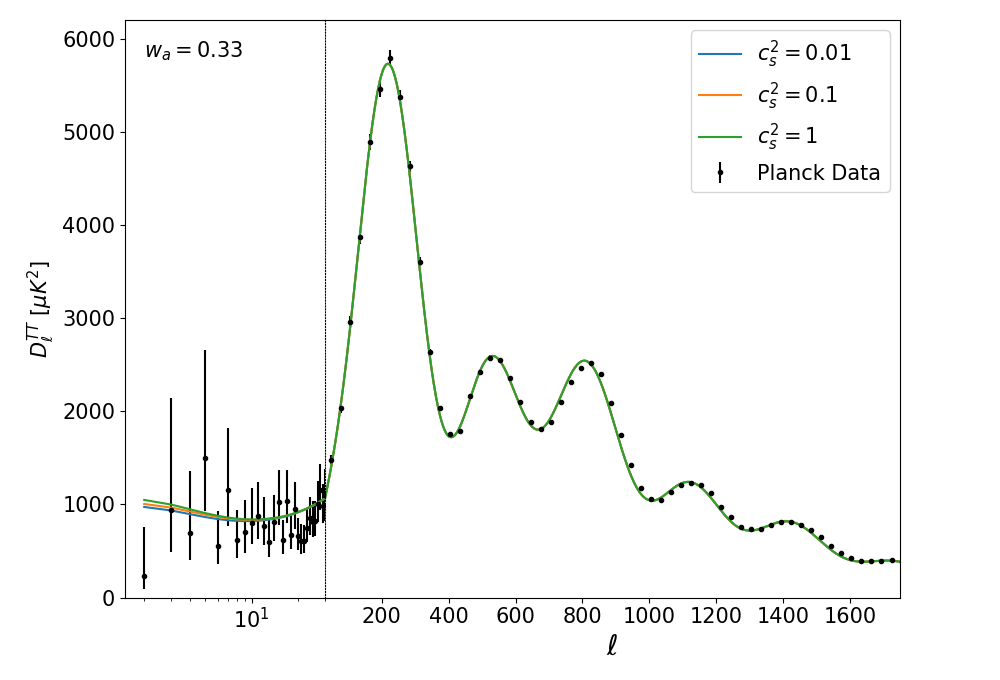
\includegraphics[width=\linewidth]{Imagens/full_doublscale_Wafixo0.33.png}
		\caption{}
		\label{fig:dark_energy_wa=0.33}
	\end{subfigure}
	\hfill
	\begin{subfigure}[t]{.43\paperwidth}
		\centering
		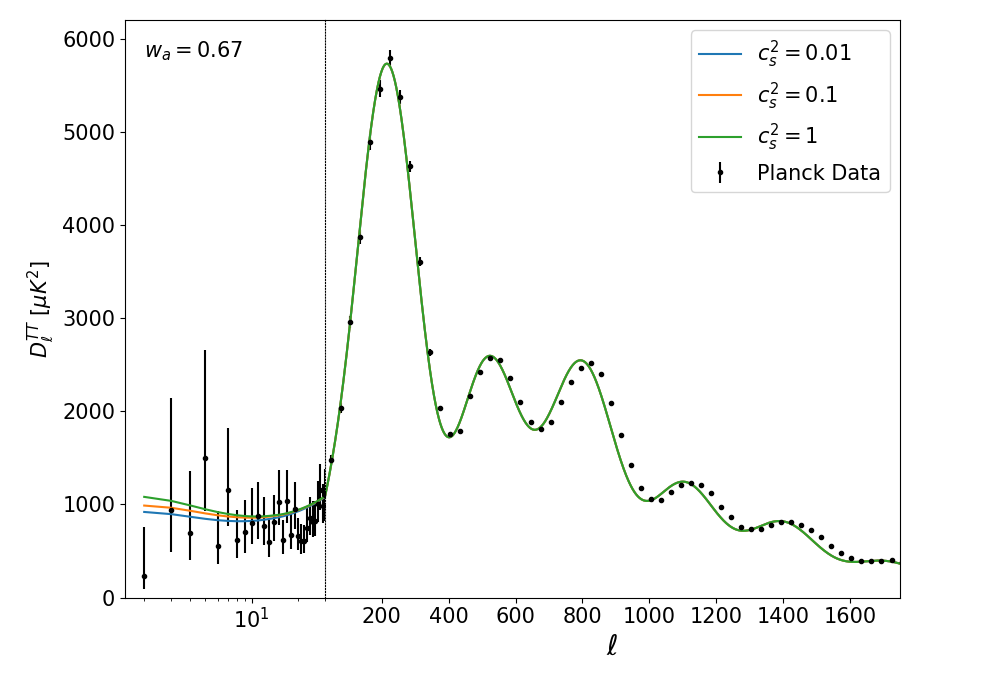
\includegraphics[width=\linewidth]{Imagens/full_doublscale_Wafixo0.67.png}
		\caption{}
		\label{fig:dark_energy_wa=0.67}
	\end{subfigure}
}	
\makebox[.87\paperwidth]{
	\begin{subfigure}[t]{.43\paperwidth}
		\centering
		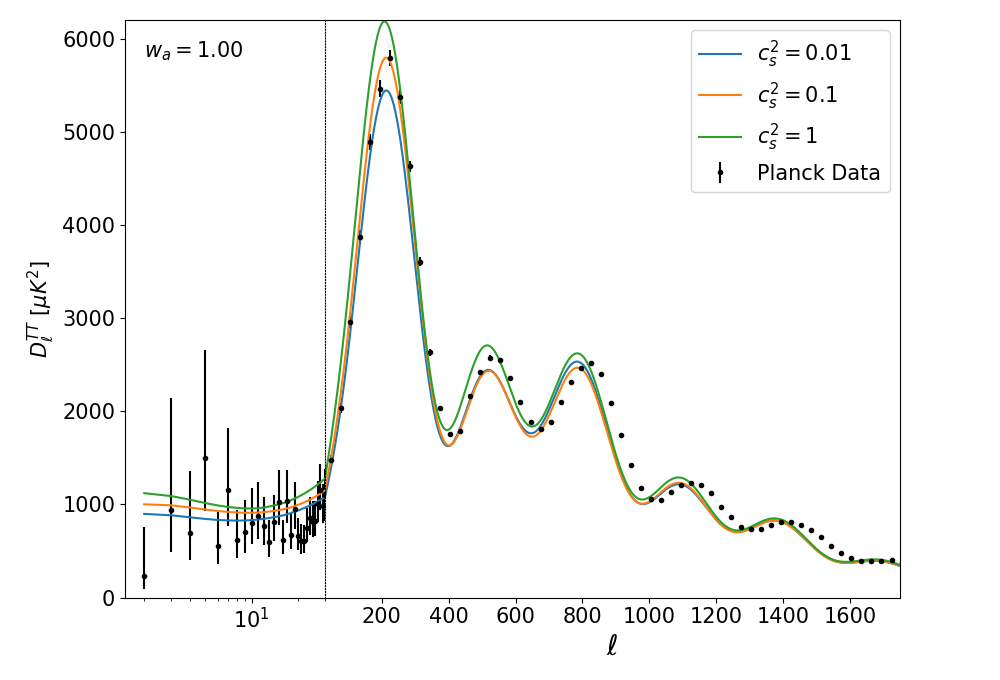
\includegraphics[width=\linewidth]{Imagens/full_doublscale_Wafixo1.00.png}
		\caption{}
		\label{fig:dark_energy_wa=1}
	\end{subfigure}
	\hfill
	\begin{subfigure}[t]{.43\paperwidth}
		\centering
		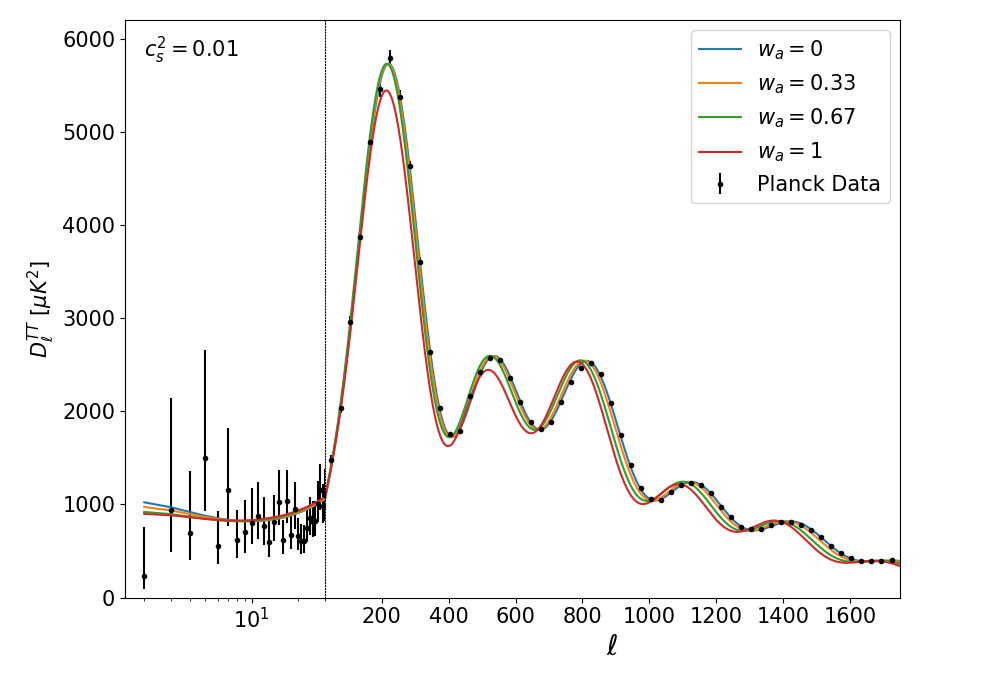
\includegraphics[width=\linewidth]{Imagens/full_doublscale_Cs2fixo0.01.png}
		\caption{}
		\label{fig:dark_energy_cs2=0.01}
	\end{subfigure}
}
	\makebox[.87\paperwidth]{
	\begin{subfigure}[t]{.43\paperwidth}
		\centering
		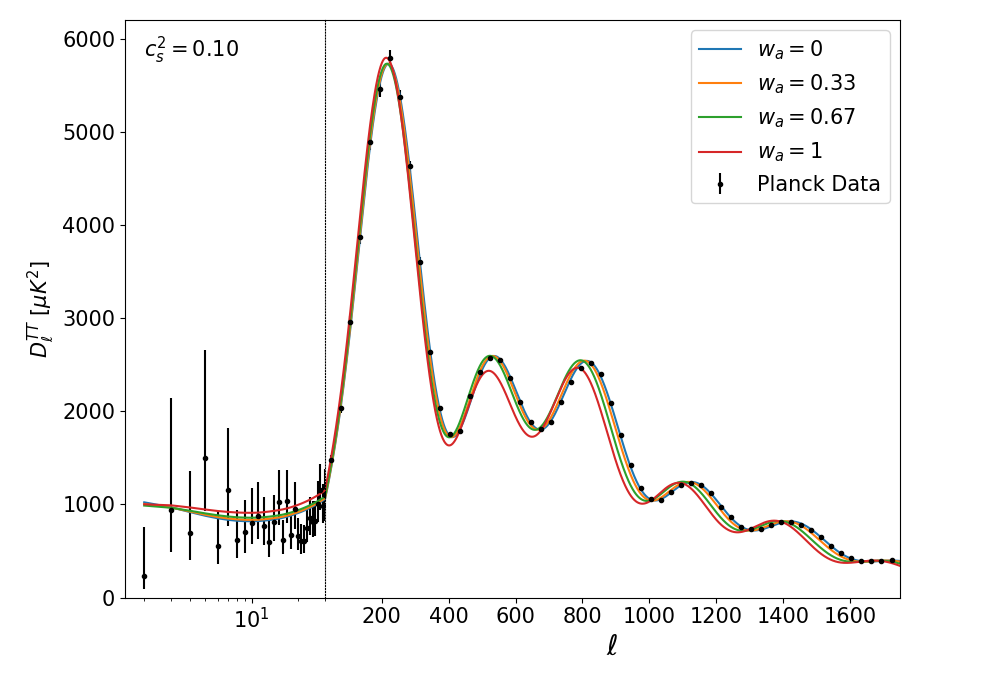
\includegraphics[width=\linewidth]{Imagens/full_doublscale_Cs2fixo0.10.png}
		\caption{}
		\label{fig:dark_energy_cs2=0.1}
	\end{subfigure}
	\hfill
	\begin{subfigure}[t]{.43\paperwidth}
		\centering
		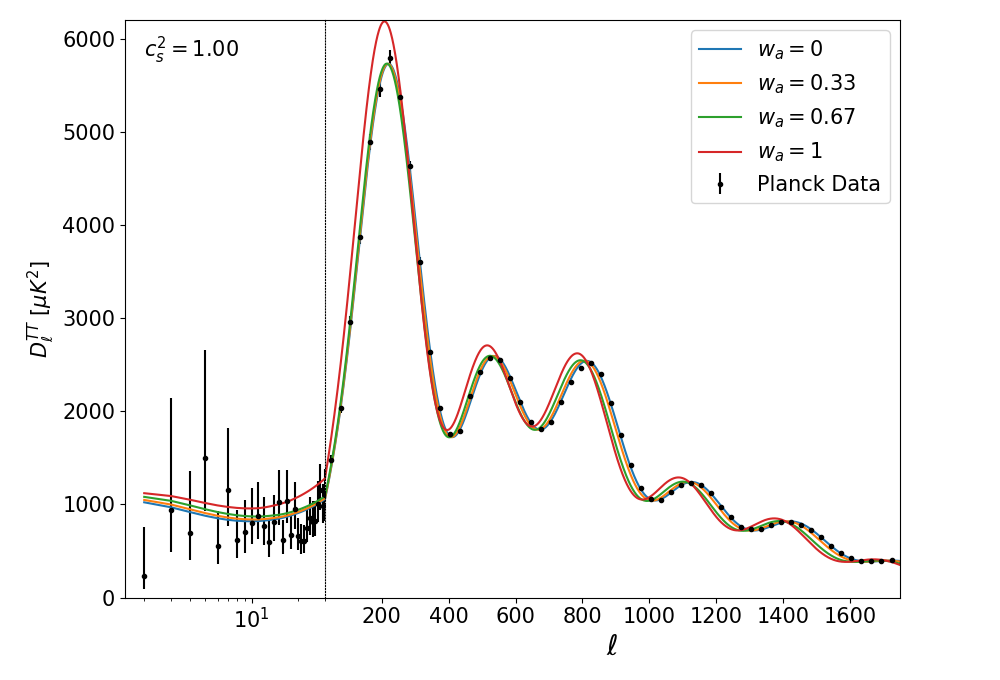
\includegraphics[width=\linewidth]{Imagens/full_doublscale_Cs2fixo1.00.png}
		\caption{}
		\label{fig:dark_energy_cs2=1}
	\end{subfigure}
}
\caption{The solid lines in the plots correspond to theoretical predictions for the CMB temperature autocorrelation spectra corresponding to different parameter values of the dark energy equation of state with $w_0=-1$, the black data points correspond to Planck's data \cite{Planck_results}. Figures \ref{fig:dark_energy_wa=0.33}, \ref{fig:dark_energy_wa=0.67} and \ref{fig:dark_energy_wa=1} show how the spectrum changes for a constant value of $w_a$ shown on the top left of the axis and varying speeds of sound, while the other three figures show how the curve behaves with varying values of $w_a$ and a constant speed of sound. All numerical calculations were done using CAMB.}
\label{fig:Dark_energy_tests}
\end{figure}

\chapter{Optimizing the Selection Function}\label{chapter:select_func_optimal}

Equation \eqref{Wg} introduced the selection function $\dv{N}{z}$, which simply corresponds to the redshift distribution of galaxy counts $N$ and can vary depending on the galaxy catalog used, thus having an influence on the expected cross-correlation and galaxy autocorrelation signals that can be extracted from that catalog. As shown in Figure \ref{fig:correlations_theoretical}, the ISW signal is mostly present at low multipoles, where cosmic variance has a strong influence, making it hard to determine whether the data follow the model or the null hypothesis of zero cross-correlation. This motivated us to study the possibility of optimizing the cross-correlation signal by determining a selection function that could theoretically maximize it, this study will be presented in this chapter.

\section{Parametrization of the Selection Function}\label{sect:sel_func_par}

Following \cite{cross_corr:Afshordi}, we are assuming the selection function can be parametrized as

\begin{equation}\label{select_func_par}
\dv{N}{z}\left(z|\lambda, \beta, z_0\right)dz=\frac{\beta}{\Gamma(\lambda)}\left(\frac{z}{z_0}\right)^{\beta\lambda-1}\text{exp}\left[-\left(\frac{z}{z_0}\right)^\beta\right]d\left(\frac{z}{z_0}\right)
\end{equation}

\noindent where the parameters $\beta$, $\lambda$ and $z_0$ are all positive. The values used to calculate the spectra in Figure \ref{fig:correlations_theoretical} are those corresponding to the so called band 1 of the 2MASS infrared galaxy catalog. Table \ref{tab:bands_2MASS} shows the parameter values for each band of this catalog, while Figure \ref{fig:2MASS_selections} shows the plots for their corresponding selection functions. The details on what each of these bands represent will be presented in chapter \ref{chapter:extracting_correlations_from_data}.

\begin{table}[!htb]
\centering
    \begin{tabular}{cccc} \hline
     Band & $z_0$ & $\beta$ & $\lambda$ \\ \hline
     1 & $0.043$ & $1.825$ & $1.524$\\
     2 & $0.054$ & $1.800$ & $1.600$ \\
     3 & $0.067$ & $1.765$ & $1.636$\\
     4 & $0.084$ & $1.723$ & $1.684$\\ \hline
    \end{tabular}
    \caption{Parameter values for the 4 bands of the 2MASS catalog. Values extracted from \cite{cross_corr:Afshordi}.}
    \label{tab:bands_2MASS}
\end{table}

\begin{figure}[!htb]
	\centering
	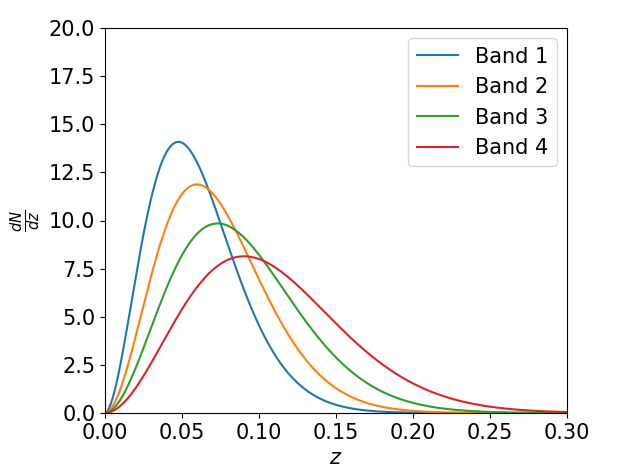
\includegraphics[width=.7\linewidth]{Imagens/selection_2MASS.png}
	\caption{Selection function calculated for the 4 bands of the 2MASS catalog according to equation \eqref{select_func_par}.}
	\label{fig:2MASS_selections}
\end{figure}

To start the search for an ideal selection function, a good first guess would be to find functions that selects galaxies at redshifts close to the period of transition to the current dark energy dominated universe. The beginning of the period of accelerated expansion can be calculated using the following equation \cite{dark_energy_era}

\begin{equation}\label{dark_energy_era_redshift}
	z^*=\left[-(1+3w_\text{de})\frac{\Omega_\text{de}}{\Omega_m}\right]^{-\frac{1}{3w_\text{de}}}-1,
\end{equation}

\noindent for which a demonstration is provided in Appendix \ref{app:dark_energy_era}. Using our $\Lambda$CDM fiducial model, i.e. using the values of Table \ref{tab:rhos&Omegas} and $w_{de}=w_\Lambda=-1$, we obtain $z^*\approx 0.63$. By analysing Figure \ref{fig:2MASS_selections}, it is possible to see that none of the 2MASS bands have peak sensitivity close to this redshift.

To determine the region in the parameter space that favors redshift $z^*$, a study of the influence of each parameter in the selection function was necessary. Figure \ref{fig:selection_tripleplot} shows how the selection function varies with changes in each of its parameters.

\begin{figure}[!htb]
	\centering
	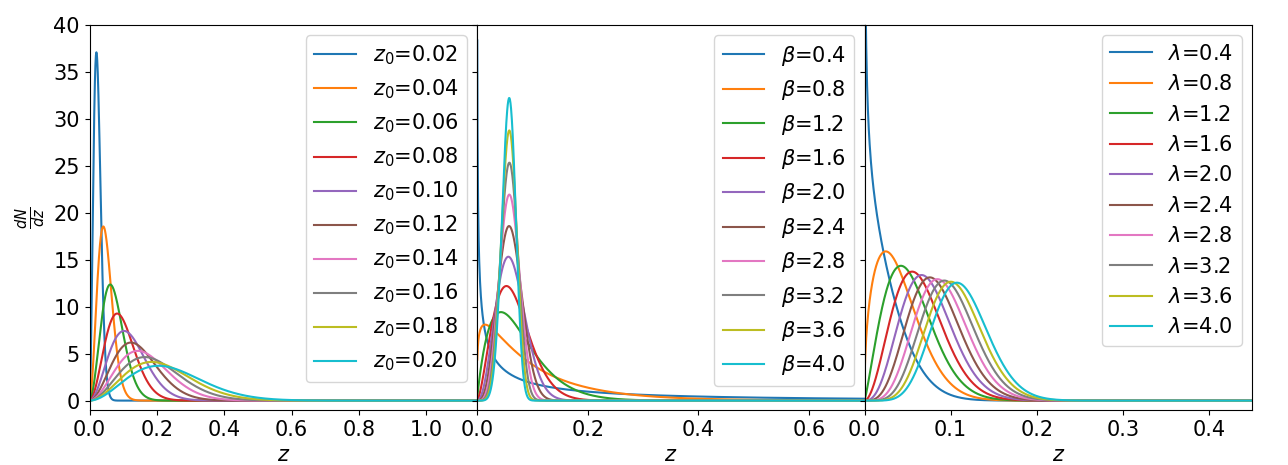
\includegraphics[width=\linewidth]{Imagens/Selection_TriplePlot.png}
	\caption{Selection function calculated for various parameter values according to the parametrization \eqref{select_func_par}. Each plot is made by keeping 2 of its three parameters fixed, corresponding to the band 2 of the 2MASS catalog (see Table \ref{tab:bands_2MASS}), the corresponding values of the varied parameter can be seen on the legend.}
	\label{fig:selection_tripleplot}
\end{figure}

Figure \ref{fig:selection_tripleplot} shows that increasing the value of $\lambda$ seems to shift the peak of the selection function towards higher redshifts without significantly changing the width of the curve, while increasing $\beta$ seems to narrow the curve without significantly changing the position of the peak, and increasing $z_0$ seems to increase both the position of the maximum and the width of the curve. 

These observations make it easier to change the parameters and see their influence on the cross-correlation signal and helps to choose a region of the parameter space to explore, but to do so, the matter of how to quantify the quality of the signal has to be discussed.

\section{Maximizing the Cross-Correlation Signal}

To maximize the signal we are in search of, we compare it with the null hypothesis, according to which there is no cross-correlation induced by the ISW effect, i.e $C^{tg}_\ell=0$ for every multipole. One way to do this is to synthesize multiple uncorrelated CMB temperature maps and galaxy contrast maps, calculate the power spectrum $C^{tg}_\ell$ for each of them and, for each multipole $\ell$, determine the distribution of $C^{tg}_\ell$, using them to determine the variance of the cross-correlation power spectrum for the null hypothesis, since their averages will be zero (within uncertainties) by construction.

In this part of the project, the HEALPix software was used extensively, and to validate the procedure for the search of the probability distribution for the null hypothesis, we first tested how the software would be able to retrieve the signal of a non-null cross-correlation spectrum. To do this, the full autocorrelation spectrum shown in Figure \ref{fig:Ctt_ISW_comparison} calculated using CAMB was used alongside the correlation spectra shown in Figure \ref{fig:correlations_theoretical} as inputs to {\it synfast}, a HEALPix harmonic space sampler and harmonic to real space map synthesizer. The synthetic maps generated with this procedure can then be decomposed into spherical harmonics coefficients $a_{\ell m}$ using {\it anafast}, another HEALPix functionality. Figure \ref{fig:SynthMaps} illustrates one galaxy contrast map and one CMB temperature map synthesized using this procedure.

\begin{figure}[!htb]
	\centering
	\begin{subfigure}[b]{0.49\textwidth}
		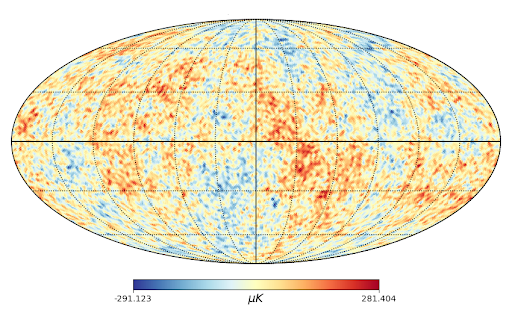
\includegraphics[width=\linewidth]{Imagens/SynthMap_CMB.png}
		\caption{CMB temperature}
		\label{subfig:CMB_synthmap}
	\end{subfigure}
	\hfill
	\begin{subfigure}[b]{0.49\textwidth}
		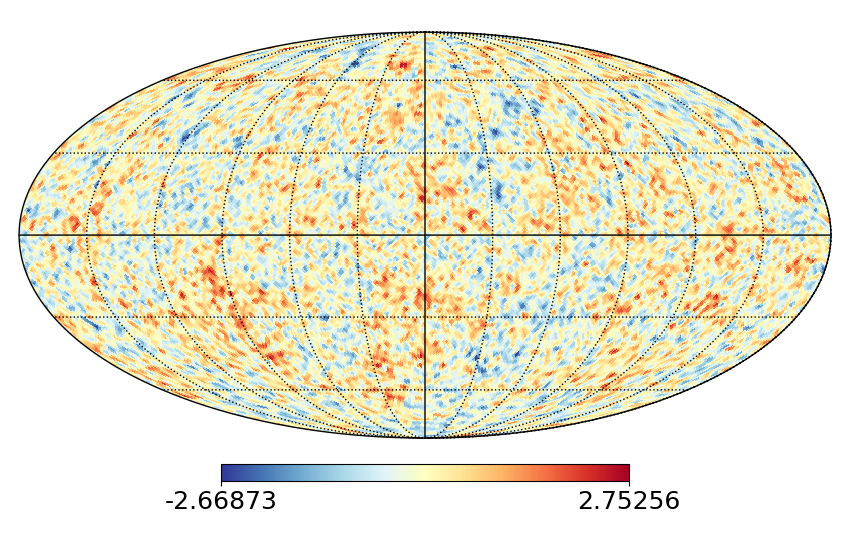
\includegraphics[width=\linewidth]{Imagens/SynthMap_Galaxy.png}
		\caption{Galaxy contrast}
		\label{subfig:galaxy_synthmap}
	\end{subfigure}
	\caption{Mollweide projection of two instances of maps synthesized using HEALPix with the procedure presented.}
	\label{fig:SynthMaps}
\end{figure} 

Figure \ref{fig:SynthMaps_AvPlots} shows a comparison between the theoretical correlation spectra and the ones estimated from averaging the correlation spectra of $10^4$ synthetic maps, showing that among the three spectra considered here, the cross-correlation is the one most affected by cosmic variance.

\begin{figure}[!htb]
\centering
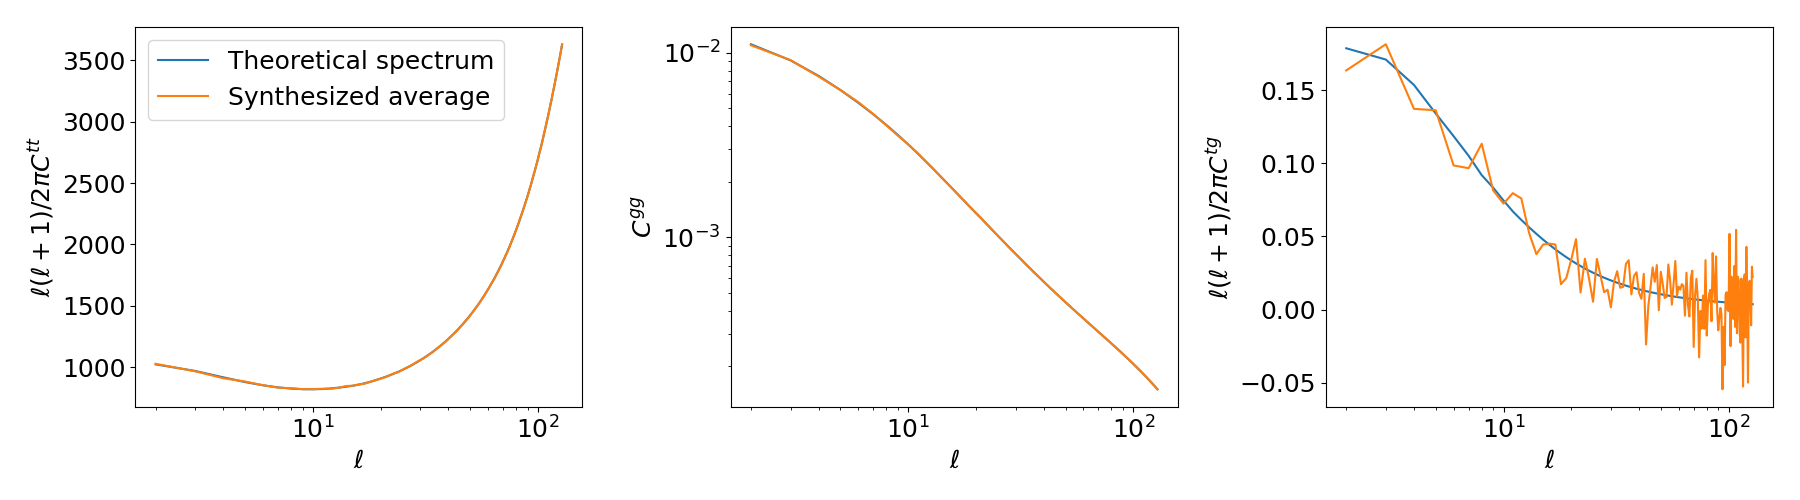
\includegraphics[width=\linewidth]{Imagens/Synth_TriplePlot.png}
\caption{Comparison between theoretical auto and cross-correlation spectra and the averages of the $C_\ell$ calculated from $10^4$ synthesized maps using the procedure presented in this section.}
\label{fig:SynthMaps_AvPlots}
\end{figure}

In order to determine the probability distribution of the null hypothesis for each multipole, a similar process can be used, but now $C^{tg}$ is set to zero, therefore, the temperature and galaxy contrast maps will be uncorrelated realizations of the autocorrelation spectra $C^{tt}$ and $C^{gg}$. For each multipole, we have a sample of $C^{tg}_\ell$, one value for each map, the distribution of these values can be used as a probability distribution for the null hypothesis at each multipole. Figure \ref{fig:synthmaps_histograms} shows two histograms representing these distributions for $\ell=4$ (left) and $\ell=30$ (right).

\begin{figure}[!htb]
	\centering
	\begin{subfigure}[b]{0.49\textwidth}
		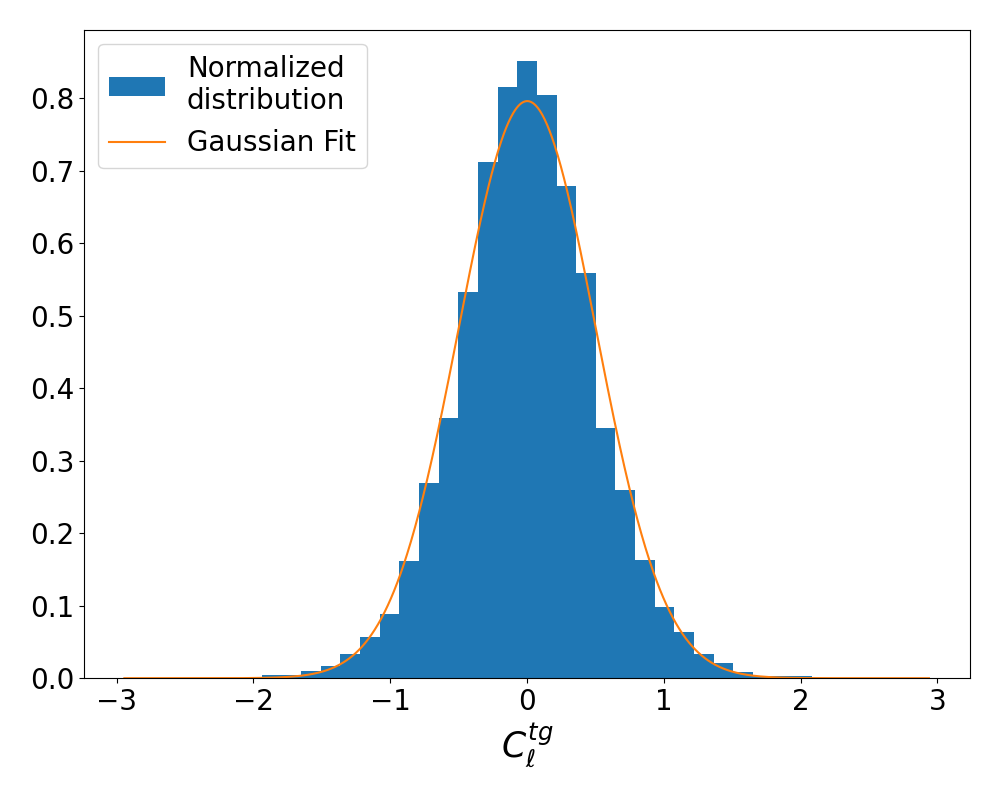
\includegraphics[width=\linewidth]{Imagens/hist_l4.png}
		\caption{Distribution for $\ell=4$.}
		\label{subfig:Hist_l4}
	\end{subfigure}
	\hfill
	\begin{subfigure}[b]{0.49\textwidth}
		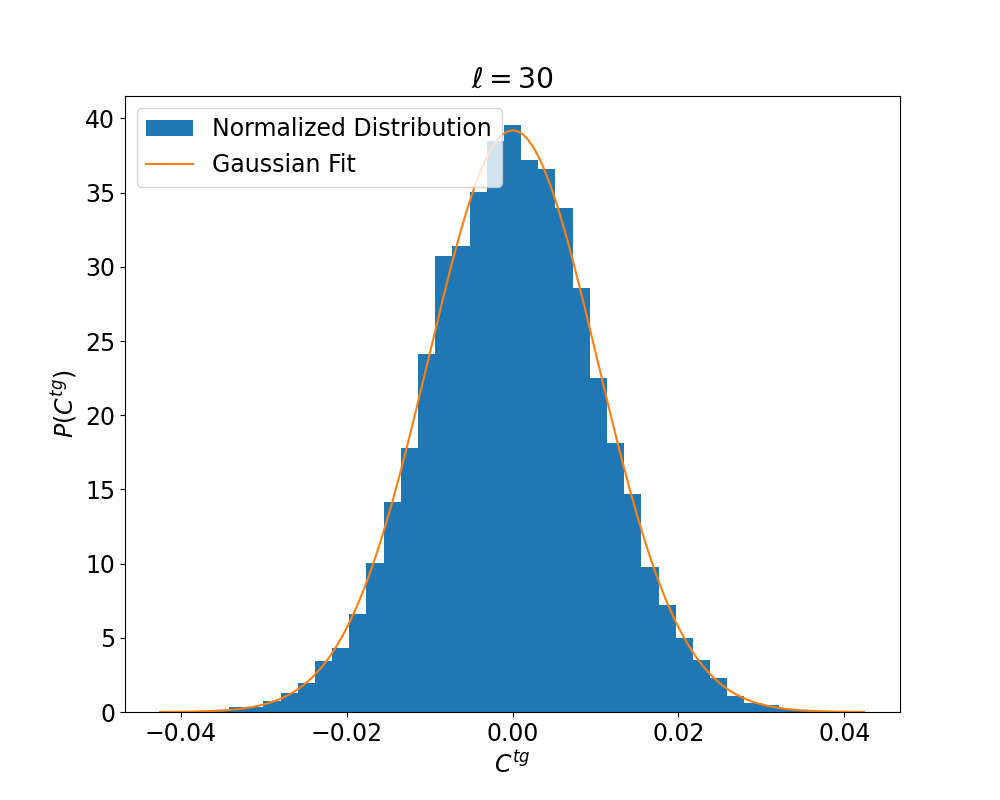
\includegraphics[width=\linewidth]{Imagens/hist_l30.png}
		\caption{Distribution for $\ell=30$}
		\label{subfig:Hist_l30}
	\end{subfigure}
	\caption{Distribution of cross-correlation values on different multipoles for $10^4$ maps synthesized with null cross-correlation. Gaussian fits of the samples are shown alongside the normalized distributions. As expected, the averages of the distributions are close to zero, and the variance of the distribution is significantly higher in low multipoles due to cosmic variance.}
	\label{fig:synthmaps_histograms}
\end{figure}

Upon thorough inspection of the histograms, we decided to fit each one using Gaussian distributions, which are shown in Figure \ref{fig:synthmaps_histograms}, and used the fitted Gaussians as the probability density functions of $C^{tg}_{\ell}$ under the null hypothesis. Each of these distributions will be indicated by $f_\ell\left(C^{tg}_\ell\right)$, so

\begin{equation}\label{f(ctgl)}
	f_\ell\left(C^{tg}_\ell\right)=\frac{1}{\sqrt{2\pi\sigma_\ell^2}}\text{exp}\left[-\frac{1}{2}\left(\frac{C^{tg}_\ell-\mu_\ell}{\sigma_\ell}\right)^2\right],
\end{equation}

\noindent where $\sigma_\ell^2$ and $\mu_\ell$ are the variance and average extracted from the distribution of $C_\ell^{tg}$ shown in Figure \ref{fig:synthmaps_histograms}.

With that, we can finally define the probability $P_\text{null}$ that a correlation spectrum $C^{tg}$ follows the null hypothesis:

\begin{equation}\label{def:Pnull}
	P_\text{null}=\prod_{\ell=2}^{\ell_\text{max}} f_\ell\left(C^{tg}_\ell\right).
\end{equation}

We can now explore the parameter space $(z_0,\beta,\lambda)$ and look for the values that minimize $P_\textbf{null}$. In other words, for a given cosmological model chosen a priori (in this case $\Lambda$CDM) where a CMB-galaxy non-null cross-correlation signal is expected, what is the selection function that minimizes the consistency with a null signal.

To perform an initial exploration of the parameter space for the parametrization \eqref{select_func_par}, 2D heat maps were produced by varying 2 of the 3 parameters while maintaining the third parameter fixed, the function mapped was $P_\text{null}(z_0, \beta,\lambda)/P_\text{null}^\text{2MASS}$, where $P_\text{null}(z_0, \beta,\lambda)$ is the probability \eqref{def:Pnull} calculated using power spectra computed with the selection function that corresponds to the given parameters, and $P_\text{null}^\text{2MASS}$ is the same probability calculated with the parameters of the band 1 of the 2MASS catalog. Figure \ref{fig:Triple_ColorPlots} shows examples of these heat maps.

\begin{figure}[!htb]
	\centering
	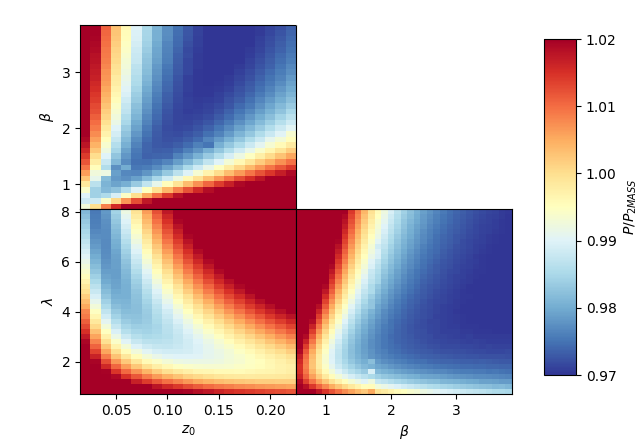
\includegraphics[width=.92\linewidth]{Imagens/triple_colorplot.png}
	\caption{For each plot, one parameter is fixed at a certain value. The color of the plot indicates the ratio $P_\text{null}(z_0, \beta,\lambda)/P_\text{null}^\text{2MASS}$, according to the bar on the right. Dark blue regions indicate the lower values of this ratio, these are the regions that improve the signal according to our analysis, and can indicate regions where a minimum value can be found. The constant values are: $\lambda=5$ (upper left), $\beta=1$ (lower left) and $z_0=0.17$ (lower right).}
	\label{fig:Triple_ColorPlots}
\end{figure}

As shown in Figure \ref{fig:Triple_ColorPlots}, the region explored does not present a significant reduction in the probability of a certain parameter combination being compatible with the null hypothesis relative to the band 1 of 2MASS, showing no more than a 3\% reduction in the ratio. In spite of this, it is possible to see a region of low values for this function where a function minimizer algorithm could possibly be able to start the search for a minimum value.

A code for minimizing the function $P_\text{null}$ using the GSL library \cite{gsl-manual} was devised, a few points were used as initial guess to the minimizer, some of them in the dark blue region, and some of them in the light blue ones, to make sure the convergence of the minimizer is reliable, and in every case results were very simillar. The final value used for our analysis was

\begin{equation}\label{minimizer}
	(\beta, z_0, \lambda)_\text{min}=(3.088, 0.1508, 4.9401)
\end{equation}

For this combination of parameters, $P_\text{null}(z_0, \beta,\lambda)/P_\text{null}^\text{2MASS}=0.971$, still a 3\% improvement relative to band 1 of 2MASS. Figure \ref{fig:minimum_properties} shows the selection and cross-correlation functions associated to the minimum of equation \eqref{minimizer}.

\begin{figure}[!htb]
     \centering
     \begin{subfigure}[b]{0.49\textwidth}
         \centering
         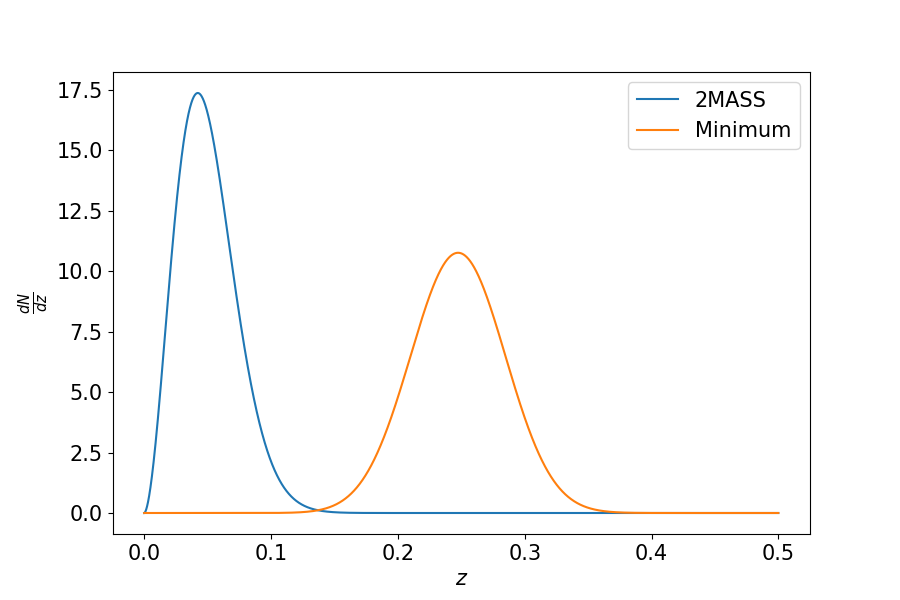
\includegraphics[width=\textwidth]{Imagens/minimum_SelFunc.png}
         \caption{Selection Function}         
         \label{subfig:minimum_SelFunc}
     \end{subfigure}
     \hfill
     \begin{subfigure}[b]{0.49\textwidth}
         \centering
         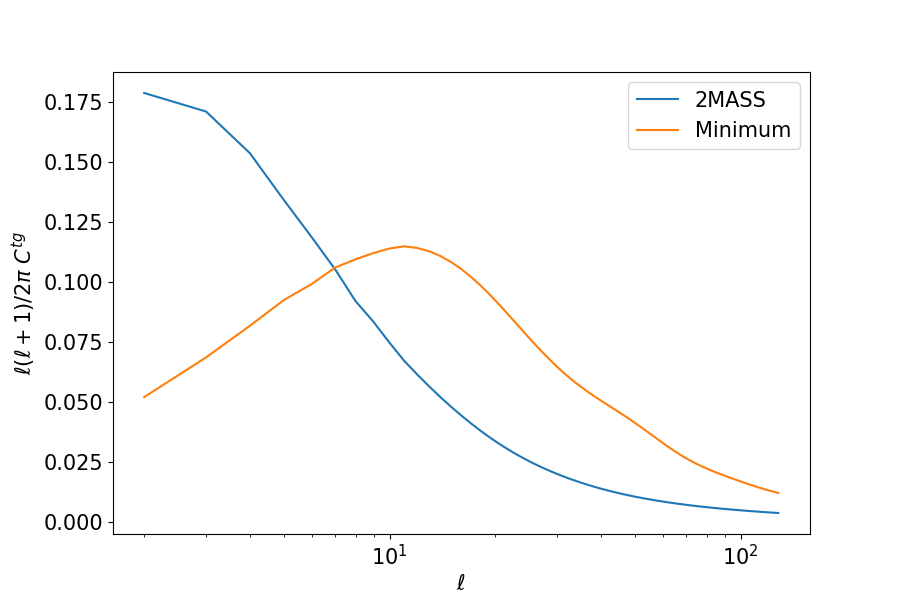
\includegraphics[width=\textwidth]{Imagens/minimumX2mass.png}
         \caption{Power Spectra}
         \label{subfig:minimum_PowSpec}
     \end{subfigure}
        \caption{Comparison between theoretical properties of the point in parameter space that minimizes the null hypothesis and that of 2MASS, band 1 in the case of Figure \ref{subfig:minimum_PowSpec}.}
        \label{fig:minimum_properties}
\end{figure}

The selection function shown in Figure \ref{subfig:minimum_SelFunc} does not favor the predicted $z^*=0.63$. This could possibly be reached by increasing the value of $\lambda$, but both the minimizer and the heat maps shown in \ref{fig:Triple_ColorPlots} indicate that not much statistical power, if any, would be gained from doing so. The power spectra comparison in Figure \ref{subfig:minimum_PowSpec} indicates an interesting tradeoff to achieve a better signal: it has a resonably higher signal at around $\ell=10$, where cosmic variance is not as relevant as it is around $\ell=2$, but the function has a lower signal at its maximum point.

Despite these insights, the statistical gains from this ideal set of parameters are not very high compared with the 2MASS signal if we assume our galaxy catalog follows the parametrization \eqref{select_func_par} and that $w_{de}=w_\Lambda=-1$. On the other hand, as we will see in Chapter \ref{chapter:constraints}, this optimized selection function leads to slightly improved constraints on the parameter $\Omega_m$ in the context of the $\Lambda$CDM model.

\chapter{Extracting Correlations from Data} \label{chapter:extracting_correlations_from_data}

%CMB experiments do not directly measure correlation spectra, instead the data consists of time ordered data streams, each stream with information of the direction of observation and the sky temperature measured by that detector, which is contained within an array of detectors. 

In this chapter, we present details on how the CMB temperature and galaxy contrast correlation spectra have been extracted from pixelized sky maps of these two observables. The data used for this purpose was measured by the Wilkinson Microwave Probe (WMAP) satellite and by the Two Micron All Sky Survey (2MASS), respectively. The contamination introduced in the maps by the strong galactic emission has to be taken into account, that is, we should deal with partial sky coverage. Noise introduced by the electronics as well as natural fluctuations due to finite galaxy counts should also be dealt with. At last, the challenge associated to the computational complexity of evaluating a likelihood in a highly dimensional parameter space will be overcome by the use of a Monte Carlo sampling algorithm.

%In this chapter, the process of converting this signal, taking into account the effects of detector noise and environmental variables such as the galactic background, will be discussed, not only for CMB but also for galaxy maps. A Monte Carlo Markov Chain (MCMC) algorithm capable of efficiently extracting these correlations, including the galaxy-CMB cross-correlation, will be presented.



\section{Data Sets and Analysis}

In this project, we have used two main datasets for our analysis: CMB data from the WMAP \cite{WMAP_results,WMAP_data} and galaxy contrast data from the 2MASS catalog \cite{2MASS}. In this section, the details about these data sets and their respective analysis pipelines will be explored. It is known that the state of the art in terms of CMB maps are nowadays provided by the Planck due to its arcminute angular resolution. However, the signal being probed here is expected to dominate at large scales, therefore WMAP and Planck data should be essentially equivalent for that purpose. On the other hand, since one is also interested in the two-point correlation functions in harmonic space of the projected CMB temperature and galaxy contrast, sky coverage is a key point in the analysis and that is the reason a galaxy survey with the largest sky coverage has been chosen here, even though the data of much deeper surveys are already available today.

\subsection{WMAP Data}

The WMAP satellite measured the CMB temperature over the entire sky in five frequency bands in the spectral region where the
CMB-to-foreground ratio is near its maximum \cite{WMAP_data}. Out of these five frequency bands, we have used in this work the data corresponding to the Q (40 GHz), V (60 GHz) and W (90 GHz) bands, which are the ones suitable for data analysis, due to their minimized galactic contamination. Its last data realease, WMAP9, which is the one used here, contains high resolution temperature intensity maps with noise power that can be well modeled as uncorrelated Gaussian fluctuations with variances given by $\sigma_0^2/N_\text{obs}$, where $\sigma_0$ is a constant characteristic of each channel (2.188 mK (Q), 3.131 mK (V) and 6.544 mK (W) \cite{wmap_supplement}) and $N_{\textrm{obs}}$ is the number of times the telescope pointed to a given direction in the sky, in other words, it is a map of the number of pointings.

Figure \ref{fig:Wmap_maps} shows the maps of the CMB temperature used for the analysis with a mask applied to them. The mask is intended to eliminate pixels highly contaminated by galactic foregrounds. The fraction of the sky that survives the masking procedure in this case is $f_{sky}=0.70$ and it is the result of combining two masks: WMAP KQ85 ($f_{sky}=0.77$) and 2MASS ($f_{sky}=0.72$). The monopole \cite{CMB_temperature:Fixsen_2009} and kinematic dipole due to the solar system movement with respect to the CMB isotropy frame have been already subtracted.

\begin{figure}[!htb]
     \centering
     \begin{subfigure}[b]{0.49\textwidth}
         \centering
         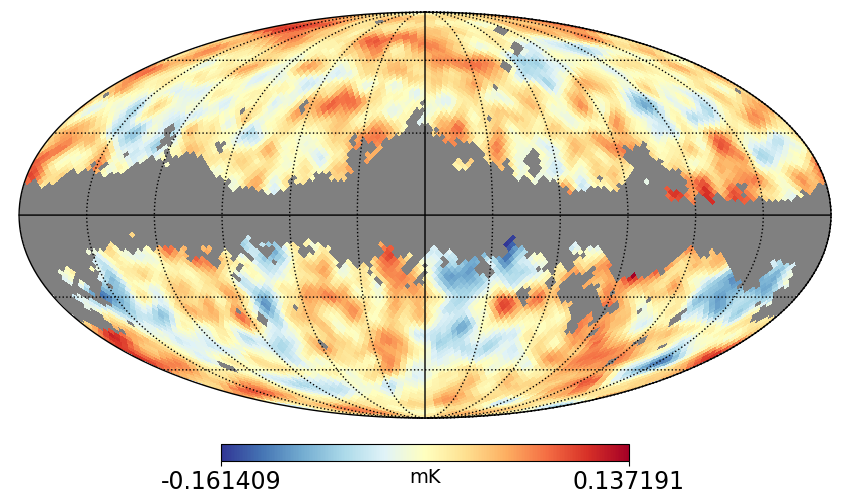
\includegraphics[width=\textwidth]{Imagens/wmap_Q_wmask.png}
         \caption{Q channel}
         \label{fig:Qchannel}
     \end{subfigure}
     \hfill
     \begin{subfigure}[b]{0.49\textwidth}
         \centering
         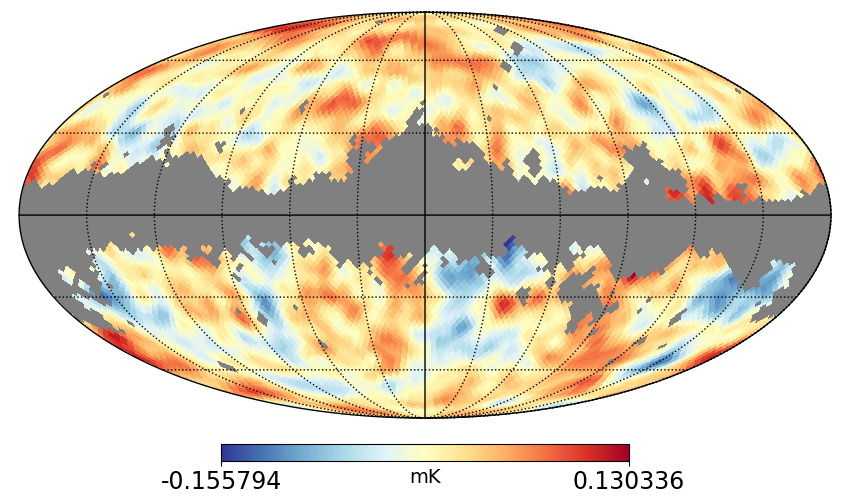
\includegraphics[width=\textwidth]{Imagens/wmap_V_wmask.png}
         \caption{V channel}
         \label{fig:Vchannel}
     \end{subfigure}
     \hfill
     \begin{subfigure}[b]{0.49\textwidth}
         \centering
         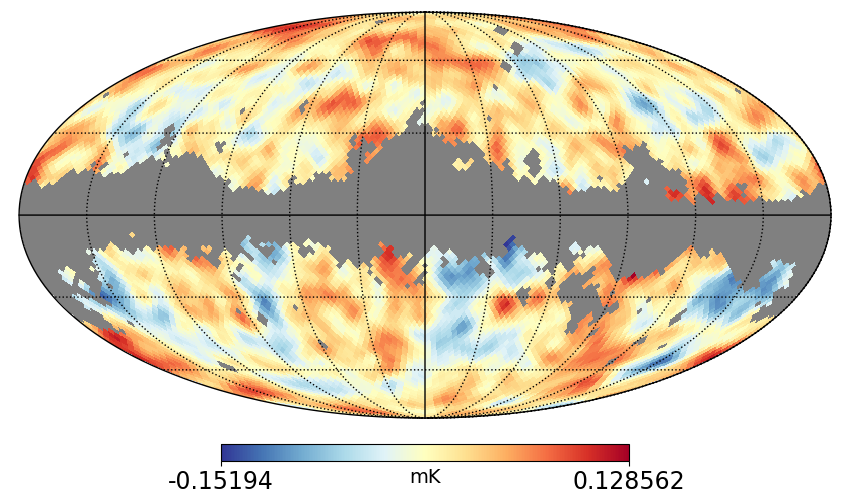
\includegraphics[width=\textwidth]{Imagens/wmap_W_wmask.png}
         \caption{W channel}
         \label{fig:Wchannel}
     \end{subfigure}
        \caption{Mollweide projection of three (Q, V, W) WMAP9 CMB temperature (in mK) maps in galactic coordinates with an $f_{sky}=0.70$ mask applied to them to exclude pixels with galactic contamination. Monopole and dipole contributions have been subtracted. The maps have HEALPix resolution correspodning to $nside$=32.}
        \label{fig:Wmap_maps}
\end{figure}

The CMB maps shown in figure \ref{fig:Wmap_maps} have also been smoothed using a Gaussian filter with a full width at half maximum (FWHM) of 5$^\circ$, to avoid sampling the signal at very high multipoles. The filtering dumps power at scales $\ell \gtrsim 20$, but also introduces correlations in the noise which are too complicated to model. Therefore, as final step in the CMB map preparation phase, regularizing uncorrelated white noise of RMS 2 $\mu$K pixel$^{-1}$ has been added to all the maps \cite{Moura-Santos_2016}. The mask, filtering and regularizing noise will be properly taken into account when extracting the correlation spectra from these maps.


\subsection{2MASS Catalog}

From 1997 to 2001, using two 1.3m dedicated telescopes at Mt. Hopkins and CTIO, Chile, 2MASS collected raw imaging data covering $99.998\%$ of the celestial sphere in three near-infrared bands: J ($\SI{1.25}{\mu \meter}$), H ($\SI{1.65}{\mu \meter}$) and $K_s$ ($\SI{2.16}{\mu \meter}$). This produced a Point Source Catalog containing more than $\SI{4.7e8}{}$ point sources and an Extended Source Catalog (XSC) of $1,647,599$ extended sources, which is the catalog we will use in this project to trace the galaxy contrast in the sky. This catalog contains sources that are extended with respect to instanteneous point source functions (PSF), such as galaxies and galactic nebulae.

The $K_s$ band's $20 \text{ mag arcsec}^{-2}$ isophotal circular aperture magnitudes (here simply called $K_{20}$) were corrected for galactic extinction using the reddening maps $E(B-V)$ at $\SI{100}{\mu \meter}$ from \cite{Schlegel_1998}, according to the expression $K_{20} \rightarrow K_{20}'=K_{20}-A_k$, where $A_k=0.367E(B-V)$.

HEALPix was used to produce and analyse the maps with resolution parameter $nside=32$, a mask was applied to every pixel with $A_k>0.05$. This left the catalog with $801,476$ objects with $12<K_{20}'<14$, which were further divided into the four bands: Bands 1 ($12.0<K_{20}'<12.5$), 2 ($12.5<K_{20}'<13.0$), 3 ($13.0<K_{20}'<13.5$) and 4 ($13.5<K_{20}'<14.0$). 

This catalog is made using photometric measurements, meaning redshift information is not directly obtained with the measurements, but there are techniques to estimate photometric redshifts. In \cite{K20_lum_func} 4192 2MASS galaxies were used to estimate the luminosity function of the entirety of the $K_s$ band, and then the photometric redshifts of these galaxies. In \cite{2MPZ} the authors trained a neural network and cross-correlated XSC with WISE \cite{WISE} and SuperCOSMOS \cite{SuperCOSMOS} to obtain the photometric redshifts of a big fraction of the sources in XSC, creating what is called the 2MPZ catalog. As shown in \cite{Moura-Santos_2016}, using the 2MPZ catalog over XSC does not yield significant changes in the results, so in this work we maintained the usage of the XSC data.

As explained in section \ref{sect:sel_func_par}, the redshift distribution of galaxy counts can be parametrized using the selection function defined in equation \eqref{select_func_par}. The selection function parametrizations for each band are shown in Table \ref{tab:bands_2MASS} and their plots as a function of redshift are shown in Figure \ref{fig:2MASS_selections}. Figure \ref{fig:2MASS_maps} shows the final galaxy contrast maps produced after smoothing them with a 5$^\circ$ FWHM Gaussian filter and adding regularizing white noise of 5\% pixel$^{-1}$ to mitigate the correlation introduced by the filtering of the original shot noise of the maps.

\begin{figure}[!htb]
     \centering
     \begin{subfigure}[b]{0.495\textwidth}
         \centering
         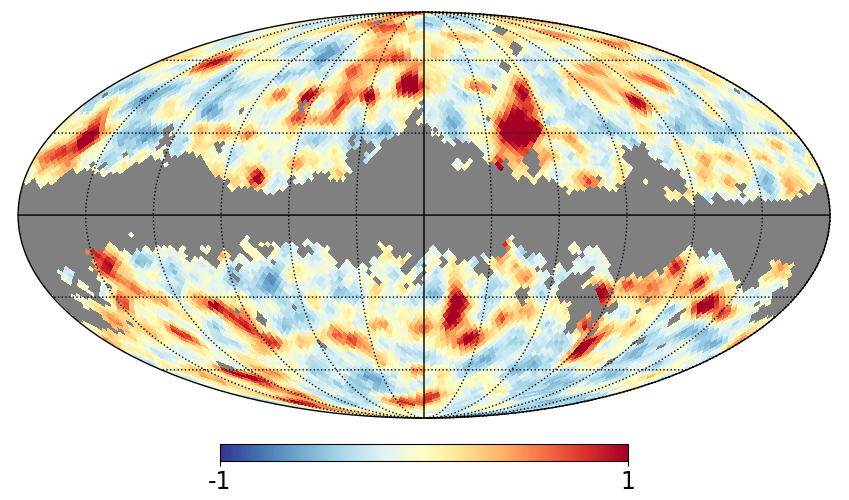
\includegraphics[width=\textwidth]{Imagens/band1_wmask_xsc.png}
         \caption{Band 1}
         \label{fig:contrast_map1}
     \end{subfigure}
     \hfill
     \begin{subfigure}[b]{0.495\textwidth}
         \centering
         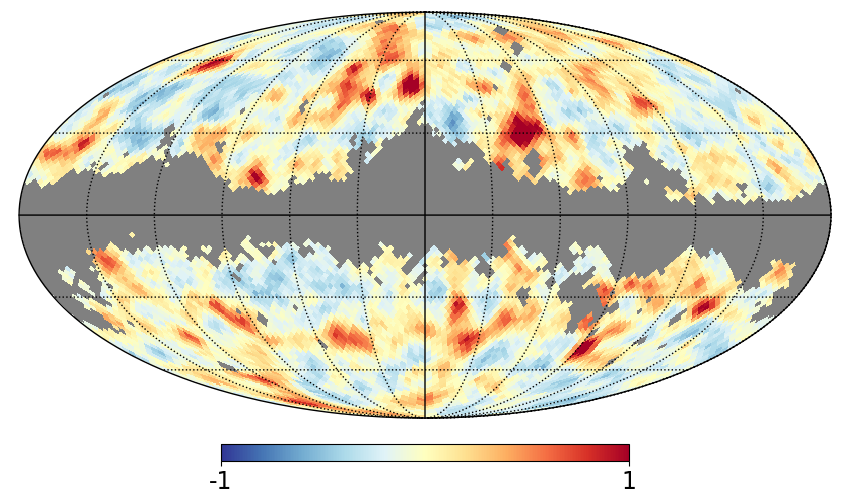
\includegraphics[width=\textwidth]{Imagens/band2_wmask_xsc.png}
         \caption{Band 2}
         \label{fig:contrast_map2}
     \end{subfigure}
     \hfill
     \begin{subfigure}[b]{0.495\textwidth}
         \centering
         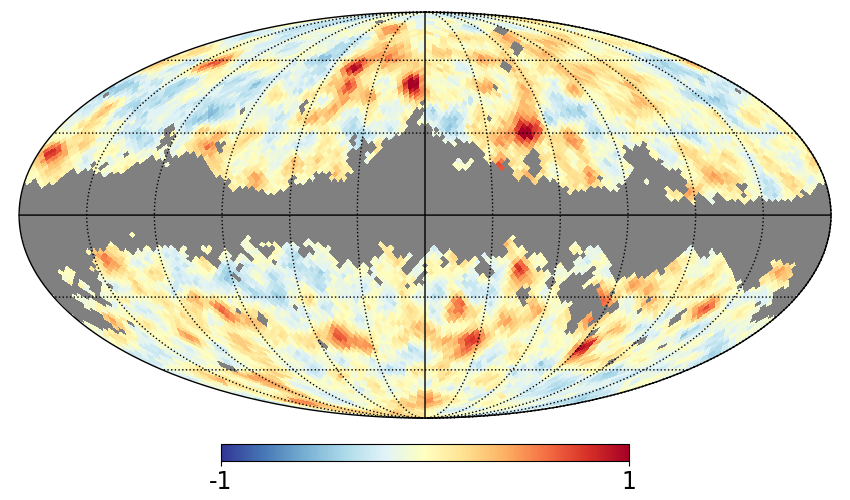
\includegraphics[width=\textwidth]{Imagens/band3_wmask_xsc.png}
         \caption{Band 3}
         \label{fig:contrast_map3}
     \end{subfigure}
     \hfill
     \begin{subfigure}[b]{0.495\textwidth}
         \centering
         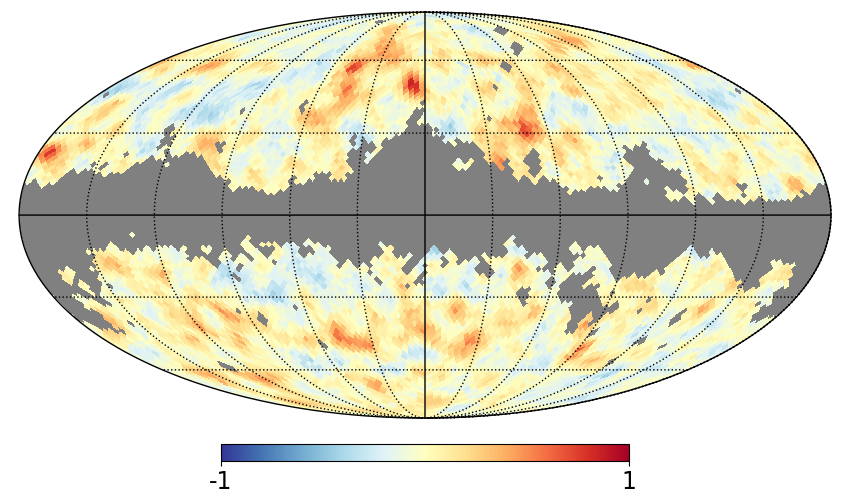
\includegraphics[width=\textwidth]{Imagens/band4_wmask_xsc.png}
         \caption{Band 4}
         \label{fig:contrast_map4}
     \end{subfigure}
     \caption{Mollweide projection of the 2MASS-XSC galaxy contrast maps in galactic coordinates with the combined 2MASS+WMAP mask applied ($f_{sky}=0.70$). Four bands are shown: band 1 ($12.0<K'_{20}<12.5$), band 2 ($12.5<K'_{20}<13.0$), band 3 ($13.0<K'_{20}<13.5$) and band 4 ($13.5<K'_{20}<14.0$). A 5$^{\circ}$ FWHM filter has been applied over the maps and regularizing white noise of 5\%  pixel$^{-1}$ RMS strength finally added.}
        \label{fig:2MASS_maps}
      \end{figure}

      
\section{Two-Point Correlaton Functions}

%To estimate any correlation spectrum, we first need to estimate the values of the multipole terms $a_{\ell m}$, but applying equation \eqref{def:autocorrelation} to these directly does not yield accurate results, one has to introduce factors such as noise and map masks first. 

The presence of the mask in the previous maps introduces a complication when calculating correlation functions such as the power spectrum. To account for the mask, in general, it is common to introduce a weight function $W(\hat{\mathbf{n}})$ which is 1 for unmasked pixels and 0 for masked ones \cite{Hivon_2002}. The spherical harmonics coefficients $\tilde{a}_{\ell m}$ obtained from these partial sky coverage maps are therefore
% If we ignore other effects for now (such as noise), the multipole terms $\tilde{a}_{\ell m}$ as defined in \eqref{ch2:alm=int...}, assuming a high number of small pixels to approximate a sum with an integral, becomes

\begin{equation}\label{ch3:tilde_a}
    \tilde{a}_{\ell m}=\int d\Omega\, \Theta(\hat{\mathbf{n}})W(\hat{\mathbf{n}})Y_{\ell m}^* (\hat{\mathbf{n}}).
  \end{equation}
  and are called pseudo spherical harmonics coefficients. Likewise, the so-called pseudo-power spectrum $\tilde{C}_\ell$ is given by:
  
\begin{equation}\label{ch3:tilde_Cl}
    \tilde{C}_\ell=\frac{1}{2\ell+1}\sum_{m=-\ell}^\ell |\tilde{a}_{\ell m}|^2.
\end{equation}

In terms of the power spectrum, the consequence of the mask is to introduce a mixing between different multipoles, that is, an artificial break of the statistical isotropy of the $a_{\ell m}$'s is introduced. It can be shown that in this situation the ensemble average of the pseudo-power spectrum is related to the true power spectrum via a system of linear equations \cite{Hivon_2002}

\begin{equation}
    \av{\tilde{C}_\ell}=\sum_{\ell'} M_{\ell \ell'} \av{C_\ell},
\end{equation}

\noindent where $M_{\ell \ell'}$ is a matrix that describes the coupling between modes introduced by the mask, called the multipole mixing matrix or mixing kernel. If the mask itself is seen as a scalar field over the 2-sphere with power spectrum given by $\mathcal{W}_\ell$, the mixing matrix $M_{\ell \ell'}$ in turn is given by

\begin{equation}
    M_{\ell \ell'}=\frac{2\ell'+1}{4\pi}\sum_{\ell''}(2\ell''+1)\mathcal{W}_\ell''
    \begin{pmatrix}
        \ell & \ell' & \ell''\\
        0 & 0 & 0
    \end{pmatrix}^2,
\end{equation}

\noindent in which the term in parenthesis is a Wigner-$3j$ symbol.

To find the full form of the system of equations used to determine the true power spectrum, one has to take into consideration the so-called beam pattern, since all astronomical observations are made with telescopes of finite angular resolution. More precisely, in an apparatus that measures CMB temperatures, the measurement in each direction $\hat{\mathbf{n}}$ is a value $T^\text{obs}(\hat{\mathbf{n}})$ corresponding to a weighted average of the real temperatures $T(\hat{\mathbf{n}} ')$:
% plus a noise $\eta(\hat{n})$:
% In radio astronomy, telescopes take measurements in various angles in the sky, and for each direction $\hat{n}$, there is an area of the sky being covered by the measurement, each of these areas is called a beam. In an apparatus that measures CMB photons' temperatures, the measurement in each direction $\hat{n}$ is a temperature $T^\text{obs}(\hat{n})$, this measurement corresponds to a weighted combination of the real temperatures $T(\hat{n}')$ over the beam:% plus a noise $\eta(\hat{n})$:

\begin{equation}\label{def:beam_pattern}
	T^\text{obs}(\hat{\mathbf{n}})=\int_\text{beam} d\Omega\, B(\hat{\mathbf{n}}, \hat{\mathbf{n}}') T(\hat{\mathbf{n}} ').
\end{equation}

The function $B(\hat{\mathbf{n}}, \hat{\mathbf{n}}')$ is called the beam pattern, it weights the contributions of photons coming from the directions around the telescope line of sight $\hat{\mathbf{n}}$, and can be estimated during the calibration of the apparatus. In many cases, it can be assumed to be Gaussian. %Figure \ref{fig:beam_pattern} shows the beam pattern for the Planck instrument at $30\text{ GHz}$.

%\begin{figure}[!htb]
%	\centering
%	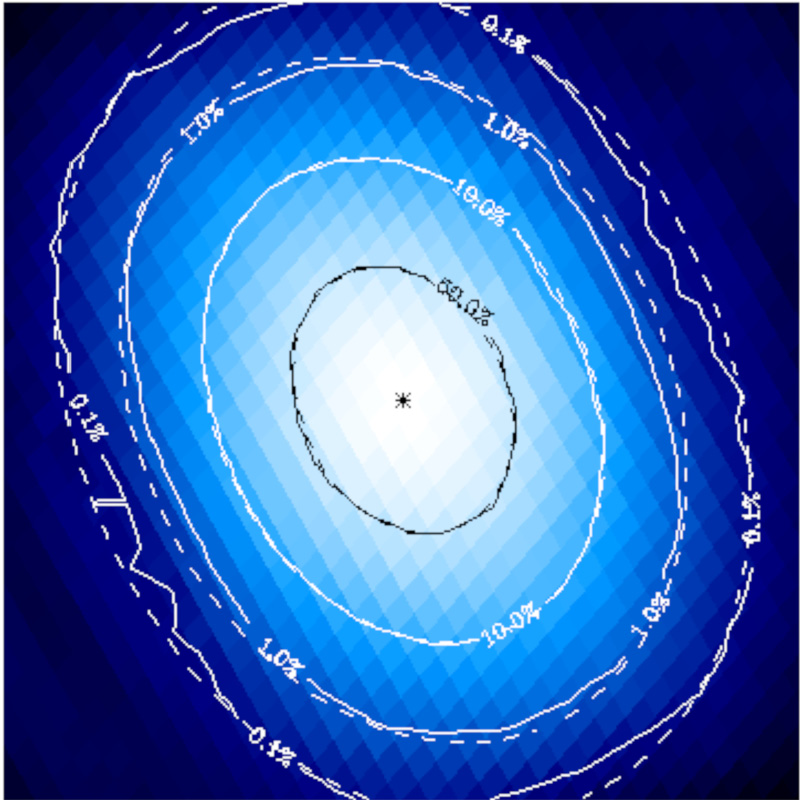
\includegraphics[width=.55\linewidth]{Imagens/beam_pattern.png}
%	\caption{Beam pattern for the Planck instrument at $30\text{ GHz}$. Contours delineate the regions where the beam function drops from its maximum to $50\%$, $10\%$, $1\%$ and $0.1\%$ respectively. Source: \href{https://wiki.cosmos.esa.int/planckpla/index.php/Effective_Beams}{Planck wiki}.}
%	\label{fig:beam_pattern}
%\end{figure}

The beam pattern itself can be seen as a scalar function over the sphere centered at the telescope line of sight. If its power spectrum is given by $B_\ell$ and given a noise map $N$ with associated power spectrum $N_\ell$, the final system of equations relating pseudo and true power spectrum ensemble average is given by:

\begin{equation}\label{ch3:av(tilde_Cl)}
    \av{\tilde{C}_\ell}=\sum_{\ell'} M_{\ell \ell'}B_{\ell'}^2\av{C_{\ell'}}+\av{N_\ell}.
\end{equation}

Equation \eqref{ch3:av(tilde_Cl)} is known as the Monte Carlo Apodized
Spherical Transform Estimator (MASTER) solution \cite{Hivon_2002}. Although this solution converges to the true power spectrum in the limit of a large number of sky realizations, having a single universe to retrieve sky map multipoles makes it highly affected by cosmic variance \cite{Moura-Santos_2016}. Another complication is the fact that for very irregular masks the mixing kernel may be singular, preventing its inversion. In some cases, a kernel regularization procedure can be applied where a binned power spectrum is introduced instead of trying to calculate $C_{\ell}$ to all multipoles $\ell$.

%Another limitation of this method is its computational complexity of $O(N_p^3)$, where $N_p$ is the number of pixels of the sample maps. For experiments such as WMAP ($N_p\sim 10^6$) and Planck ($N_p \sim 10^7$), this time complexity becomes computationally unviable, thus motivating the introduction of a new technique, which will be presented now.


\section{A likelihood-based estimator}

In order to properly take into account intrinsic fluctuations such as cosmic variance and shot noise, an approach based on a likelihood where the probability density of these fluctuations is naturally incorporated can be used instead of the MASTER approach described in the previous section. To be more precise, one is interested in reconstructing the a posteriori probability distribution of the two-point correlation functions given some data available in the form of pixelized sky maps.

%For a more efficient method than the one presented previously, Monte Carlo (MC) methods to sample maps of the primordial signal from the a posteriori probability distribution taking into account cosmic variance, instrumental noise, and residual foregrounds were developed\cite{Jewell_2004,Eriksen_2004,Wandelt_2004}. 

For example, let $d$ be a pixelized temperature map consisting of primordial signal $\mathbf{s}$ and instrumental noise $\mathbf{n}$, both following Gaussian distributions with covariance matrices $\mathbf{S}$ and $\mathbf{N}$ respectively, such that the full covariance matrix is $\mathbf{C}=\mathbf{S}+\mathbf{N}$. The likelihood for observing such a map, after marginalizing over the unknown true temperature signal $\mathbf{s}$, is given by

\begin{equation}\label{ch4:Likelihood}
	\mathcal{L}=P(\mathbf{d}|\mathbf{C})=\frac{1}{(2\pi)^{n_\text{dim}/2}|\mathbf{C}|^{1/2}}\text{exp}\left(-\frac{1}{2}\mathbf{d}^T \mathbf{C}^{-1} \mathbf{d}\right),
\end{equation}

\noindent where $n_\text{dim}=N_p^2$. The direct evaluation of this likelihood is not computationally viable due to the calculation of the determinant of $\mathbf{C}$, a matrix that cannot be represented in diagonal form, since $\mathbf{N}$ is typically close to diagonal in pixel space and $\mathbf{S}$ is diagonal in harmonic space. The computational complexity of the operaton is $O(N_p^3)$, where $N_p$ is the number of pixels of the sample maps. For experiments such as WMAP ($N_p\sim 10^6$) and Planck ($N_p \sim 10^7$), the problem becomes computationally unviable, thus motivating the introduction of a new technique, which will be presented now.

Using Bayes' theorem, we can write

\begin{equation}\label{ch4:bayes}
  P(\mathbf{C}|\mathbf{d})\propto \pi(\mathbf{S})P(\mathbf{d}|\mathbf{C}),
\end{equation}

\noindent where $\pi(\mathbf{S})$ is the prior probability on the power spectrum and $P(\mathbf{C}|\mathbf{d})$ is the posterior probability density. Sampling from \eqref{ch4:bayes} can be done using standard Monte Carlo Markov Chain methods such as those based on the Metropolis-Hastings algorithm. For the particular case of the likelihood in equation \eqref{ch4:Likelihood}, for which a set of conditional probabilities can be more directly used for sampling, the so called Gibbs sampling technique is efficient and useful for the problem at hand and has been succesfully implemented for CMB experiments in \cite{Jewell_2004,Eriksen_2004,Wandelt_2004, Larson_2007}. 

% Sampling from $P(\mathbf{C}|\mathbf{d})$ can be done using a Monte Carlo method called Gibbs sampling.
Suppose we can sample from the conditional probabilities $P(\mathbf{C}|\mathbf{s}, \mathbf{d})$ and $P(\mathbf{s}|\mathbf{C}, \mathbf{d})$. In this case, one can then sample a set of $\{(\mathbf{s}^i, \mathbf{C}^i)\}$ by iterating the following sampling process \cite{Chu_2005}:

\begin{equation}\label{gibbs_sample1}
\mathbf{s}^{i+1}\leftarrow P(\mathbf{s}|\mathbf{C}^i, \mathbf{d}),
\end{equation}
\begin{equation}\label{gibbs_sample2}
\mathbf{C}^{i+1}\leftarrow P(\mathbf{C}|\mathbf{s}^{i+1}, \mathbf{d}).
\end{equation}

From this sample, one can use the so called Blackwell-Rao estimator to determine an approximation for $P(\mathbf{C}|\mathbf{d})$ \cite{Chu_2005}. To construct this estimator, we first expand each element of the vector $\mathbf{s}$ in terms of spherical harmonics:

%has an estimation of $P(\mathbf{C}, \mathbf{s}|\mathbf{d})$, thus only needing to marginalize over $\mathbf{s}$ to obtain the posterior distribution $P(\mathbf{C}|\mathbf{d})$. To do this marginalization, one can use the so called Blackwell-Rao estimator\cite{Chu_2005}.

\begin{equation}\label{s_harmonics}
	\mathbf{s}(\theta, \phi)=\sum_{\ell=0}^{\ell_\text{max}} \sum_{m=-\ell}^\ell \mathbf{s}_{\ell m}Y_{\ell m}(\theta, \phi),
\end{equation}

\noindent and define

\begin{equation}\label{sigma_l}
	\sigma_\ell=\frac{1}{2\ell+1}\sum_{m=-\ell}^\ell \mathbf{s}_{\ell m}\mathbf{s}_{\ell m}^{\dagger}.
\end{equation}

%Next, we note that

%\begin{equation}\label{P=P=P}
%	P(C_\ell(\theta)|\mathbf{s}, \mathbf{d})=P(C_\ell(\theta)|\mathbf{s})=P(C_\ell(\theta)|\sigma_\ell).
%\end{equation}

%The first equality holds due to $C_\ell$ only depending on the signal, and the second holds because 

With this, it is possible to derive the Blackwell-Rao estimator for the density $P(C_\ell|\mathbf{d})$:

\begin{equation}\label{BR_estimator}
	P(C_\ell|\mathbf{d})\approx \frac{1}{N_G}\sum_{i=1}^{N_G}P(C_\ell|\sigma_\ell^i),
\end{equation}

\noindent where $N_G$ is the number of Gibbs samples and $C_\ell$ are the multipole values due to the true signal $\mathbf{s}$.

The previous Gibbs sampling approach for a CMB experiment has been extended in \cite{Moura-Santos_2016} to deal with the problem of estimating the full two-point correlation function of a combined CMB-galaxy survey experiment. In the extended framework, the vector $\mathbf{s}$ and the matrix $\mathbf{S}$ are defined as

%In this project, the same process presented in \cite{Moura-Santos_2016}, which is an extended version of what is presented in \cite{Larson_2007}, has been used. In this framework, the vector $\mathbf{s}$ and the matrix $\mathbf{S}$ are defined as

\begin{equation}\label{vec_s}
	\mathbf{s}^T=(s_{00}^{tg}, s_{01}^{tg}, s_{11}^{tg}, \dots, s_{\ell_\text{max}0}^{tg}, \dots, s_{\ell_\text{max} \ell_\text{max}}^{tg}),
\end{equation}
\begin{equation}\label{matrix_S}
	\mathbf{S}=\text{diag}(S_0^{tg}, S_1^{tg}, S_1^{tg},\dots, S_{\ell_\text{max}}^{tg}, \dots, S_{\ell_\text{max}}^{tg}),
\end{equation}

\noindent where the entries of the vector above are now 2-component vectors $\mathbf{s}_{\ell m}^{tg}$ containing the CMB temperature and the galaxy contrast spherical harmonics coefficients and $2\times 2$ signal correlation matrices $\mathbf{S}_\ell^{tg}$ including both the diagonal auto-correlations of CMB and galaxy contrasts as well as off-diagonal terms representing the cross-correlation between CMB and galaxy contrast which is a key observable in this work:

\begin{align}\label{s_lm=}
	\mathbf{s}_{\ell m}^{tg}&=
	\begin{pmatrix}
	a_{\ell m}^t\\
	a_{\ell m}^g
	\end{pmatrix}, &
	\mathbf{S}_\ell^{tg}&=
	\begin{pmatrix}
	C_\ell^{tt} & C_\ell^{tg}\\
	C_\ell^{tg} & C_\ell^{gg}
	\end{pmatrix}.
\end{align}

It is also assumed that the noise's covariance matrix is diagonal: $N=\text{diag}(N_{11}^{tg}, \dots, N_{ii}^{tg}, \dots, N_{pp}^{tg})$ where

\begin{equation}\label{Niitg}
	N_{ii}^{tg}=
	\begin{pmatrix}
	N_{ii}^{tt} & 0 \\
	0 & N_{ii}^{gg}
	\end{pmatrix},
\end{equation}

\noindent since the noises affecting the temperature anisotropies (due to the electronics) and galaxy contrast (Poissonian shot noise) are uncorrelated. 



\section{Correlation Spectra Obtained}

It was verified in \cite{Moura-Santos_2016} that fixing the monopole and dipole terms at 0 in the Gibbs chain results in anomalous states at those scales, so the WMAP9 maps were decomposed, and the results obtained for $C_0^{tt}$ and $C_1^{tt}$ were taken and fixed along the chain. A study of the systematic errors was also made in the same reference. 

To estimate the cosmic variance contribution on a masked map, or any map without full sky coverage, equation \eqref{cosmic_variance} has to be modified to take into account the effective sky fraction $f_{\text{sky},\ell}$, obtaining the following equation for the cosmic variance affecting $C_\ell^{xx}$ of the given spectrum \cite{wmap_supplement}: 

\begin{equation}\label{data_cosmic_variance}
	(\Delta C_\ell^{xx})_\text{cv}=\frac{C_\ell^{xx}}{f_{\text{sky},\ell}}\sqrt{\frac{2}{2\ell+1}}.
\end{equation}

Here, $C_\ell^{xx}$ can be substituted by either $C_\ell^{gg}$ or $C_\ell^{tt}$, but it can also be substituted by $D_\ell^{tt}=\ell(\ell+1)/2\pi C_\ell^{tt}$ in both sides of the equation. For the cross-correlation $C_\ell^{tg}$, the equation is adapted to

\begin{equation}\label{cosmic_variance_cross}
	(\Delta C_\ell^{tg})_\text{cv}=\sqrt{\frac{2}{2\ell+1}\frac{C_\ell^{tt}C_\ell^{gg}+(C_\ell^{tg})^2}{f_{\text{sky},\ell}^2}}.
\end{equation}

The procedures discussed so far in this chapter have already been done, more specifically the Gibbs sampling has already been done in \cite{Moura-Santos_2016} and all the data has been digitally stored and provided to be used in this project. Figure \ref{fig:correlation_data_final_plots} shows a comparison between the expected theoretical correlation spectra for a $\Lambda$CDM model and the ones calculated from real data coming from the combined 2MASS / WMAP Q, V, W channels, alongside cosmic variance bands. It is important to note that the solid curves do not represent fits to the data.

\begin{figure}[!htb]
	\centering
	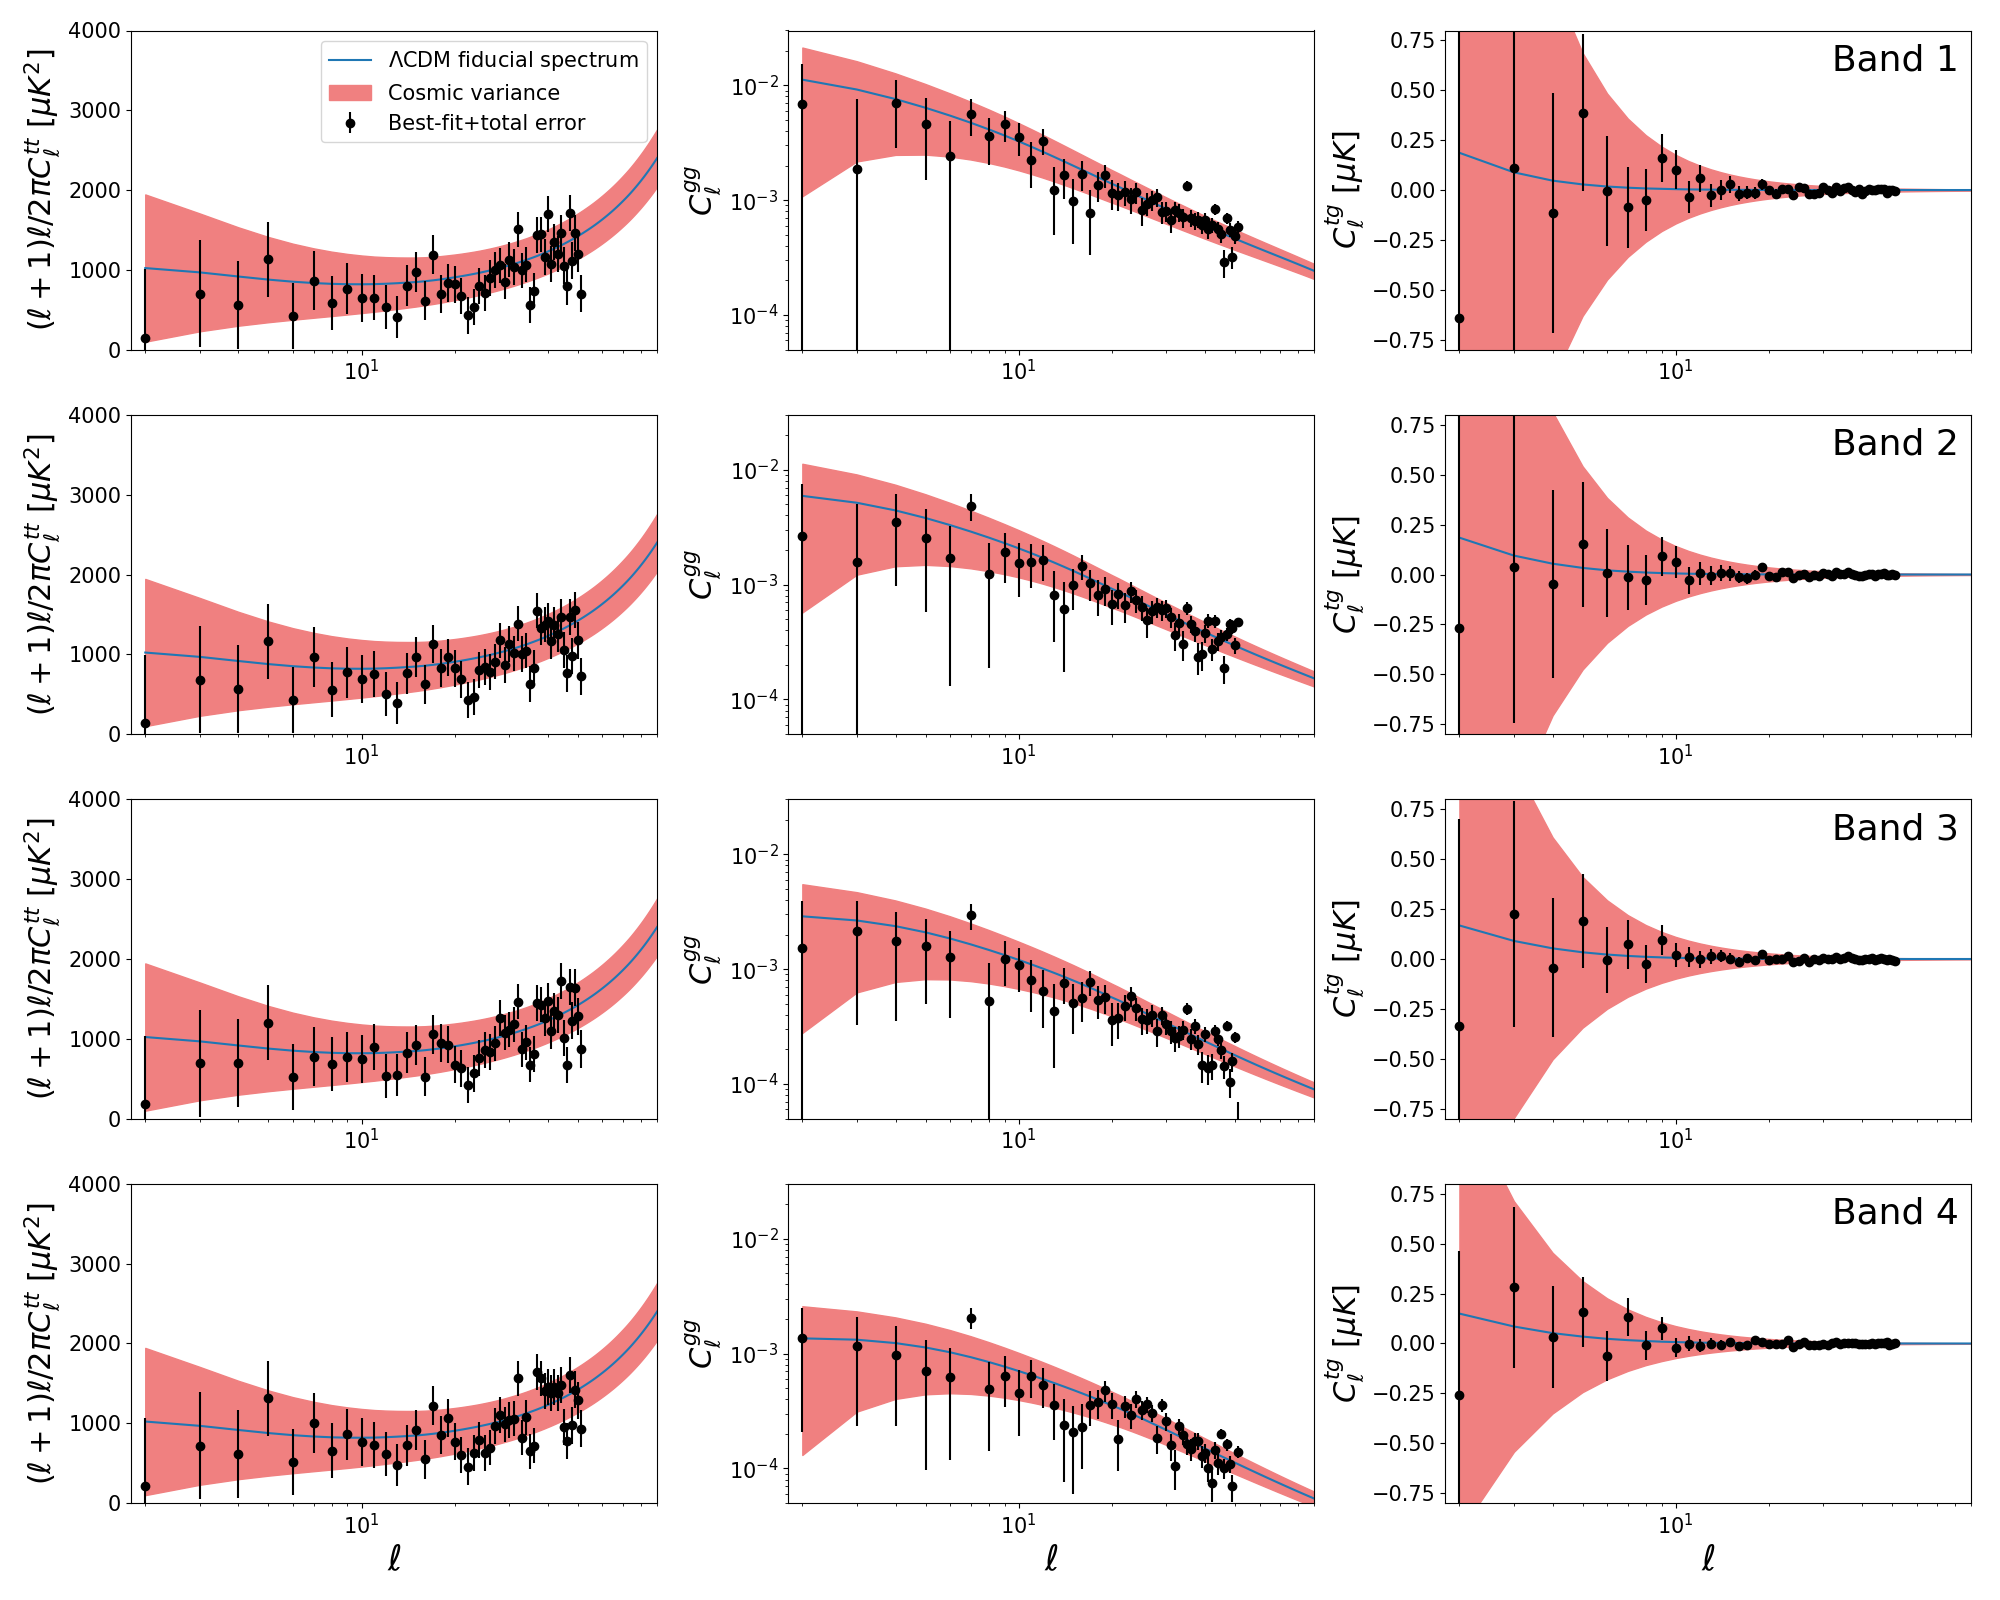
\includegraphics[width=\linewidth]{Imagens/Full_Data_Plot.png}
	\caption{Comparison of theoretical correlation spectra for each band of the 2MASS catalog and the estimated correlation values using the method presented in the current chapter. Data points with error bars are the weighted average for channels Q, V, and W, with weights given by the reciprocal of noise variances. The red band corresponds to the cosmic variance, calculated using equations \eqref{data_cosmic_variance} and \eqref{cosmic_variance_cross}. Data points are those obtained in \cite{Moura-Santos_2016}.}
	\label{fig:correlation_data_final_plots}
\end{figure}

Figure \ref{fig:correlation_data_final_plots} clearly shows that cosmic variance strongly dominates the signal at low multipoles, the region that is most influenced by the ISW effect.


\chapter{Cosmological Constraints}\label{chapter:constraints}

In this chapter we study the constraints obtained when the CMB-galaxy cross-correlation as well as the galaxy auto-correlation signals, extracted from real data as shown in the last chapter, are used in a suitable likelihood. Given the dependence of the Sachs-Wolfe effect with the background cosmology, we chose as cosmological parameter in this chapter the energy density parameter associated to non-relativistic matter $\Omega_m$.

\section{Monte Carlo Markov Chains}

The usage of MCMC methods for analysing data has become a standard practice in recent years.  These methods are usually based on the Bayes theorem, which states that the conditional probability $P(A|B)$ of occurrence of event $A$ given that event $B$ happened satisfies

\begin{equation}\label{bayes_theorem}
	P(A|B)P(B)=P(A)P(B|A).
\end{equation}

In the context of Bayesian probability, non-conditional probabilities are called prior probabilities, they describe the probability of a certain event prior to any extra information that affects that event. One can solve equation \eqref{bayes_theorem} for $P(A|B)$, in which case it is called a posterior probability, and $P(B|A)$ is called a likelihood, and is usually represented by $\mathcal{L}(B|A)$.

To generate points for a Monte Carlo Markov Chain, one uses the current state $s^i$ of the chain and samples the next value $s^{i+1}$ using a conditional probability $P(s^{i+1}|s^i)$.

In a very general sense, three main probability functions are required to run an MCMC algorithm for this type of problem: 

\begin{itemize}
	\item The joint-likelihood function: The joint-likelihood function $\mathcal{L}(Y|\theta)$ is the probability that the data points $Y$ follow the model for a certain set of parameters $\theta$. This distribution will heavily depend on the properties of the dataset and the instruments;
	\item The prior distributions: A prior distribution on the parameters $p(\theta)$ has to be assumed, possibly based on the physical properties of the parameters. If the prior is flat, one can simply use $p(\theta)=1$;
	\item The proposal distribution: This probability will determine the transition probability from one point of the chain to the next, which -- to satisfy the so called Markov Property -- only depends on the current state of the chain. Usually a Gaussian distribution is used as the proposal.
\end{itemize}

The stationary distribution of the Markov chain will be the posterior probability distribution

\begin{equation}\label{posterior_MCMC}
	P(\theta|Y)=\mathcal{L}(Y|\theta)p(\theta),
\end{equation}

\noindent of a certain set of parameter values applied to the theory correctly describing the data $Y$. 

Cobaya\cite{Cobaya_preprint, CobayaASCL} is a Python package designed to run MCMC chains to analyse any type of data desired, it is integrated with many sets of cosmological datasets and numerical packages, such as Planck's data and CAMB. 
 
Figure \ref{fig:cobaya_test}, for example, shows the  posterior probability distributions for a set of cosmological parameters of the $\Lambda$CDM model obtained after running an MCMC chain using the package Cobaya. As shown in the figure, different input data to the chain were used either separately or combined, to know:

\begin{itemize}

\item the CMB intensity  autocorrelation power spectrum (TT);

\item the CMB E-mode polarization  autocorrelation power spectrum (EE);

\item the CMB intensity-polarization cross-correlation spectrum (TE);

\end{itemize}

The 68\% and 95\% confidence levels (CL) are shown in different color intensities. One can see that the combined likelihood produces the tighter cosmological constraints. The reader can verify the consistency of the 68\% CL regions of Figure \ref{fig:cobaya_test} with the central values presented in Table \ref{tab:planck_parameters}.

\begin{figure}[!htb]
	\centering
	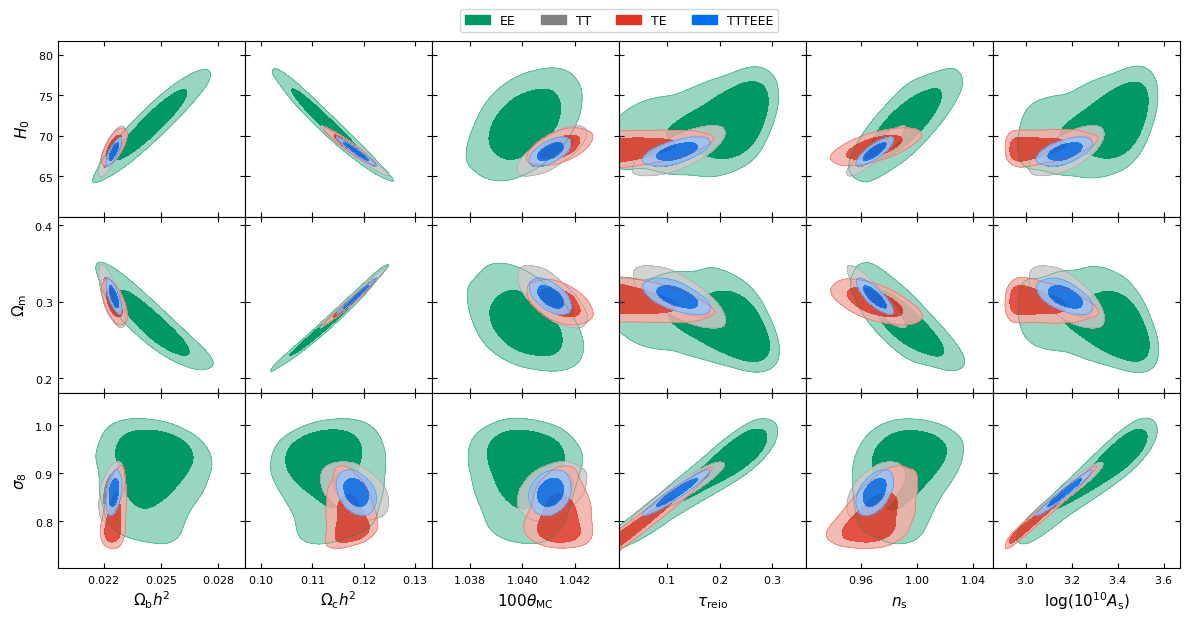
\includegraphics[width=\linewidth]{Imagens/compare_likelihoods.png}
	\caption{Joint posterior distributions of cosmological parameters using Planck's CMB temperature (T) and polarization (E) data. The TTTEEE dataset combines both autocorrelation data (TT and EE) and the cross-correlation data (TE).}
	\label{fig:cobaya_test}
\end{figure}

Cobaya uses the Gelman-Rubin Diagnostic \cite{Rminus1_paper92} to test the convergence of the chains. We have used $R-1=10^{-2}$ as a convergence criteria for the MCMC runs whose posteriors are represented in Figure \ref{fig:cobaya_test}.

To determine the parameter constraints that can be obtained from the correlation spectra discussed so far, we have used the data points of the center ($C^{gg}$) and left ($C^{tg}$) columns of Figure \ref{fig:correlation_data_final_plots}. The theoretical calculations had to be integrated within Cobaya, so we have created a Python wrapper capable of calling the C++ functions we have used to calculate the theoretical correlation spectra, the functions defined in this code could then be called in other scripts, including any using Cobaya. 

The integrals to obtain the theoretical spectra (see equation \eqref{Cl_direct_calculation}) are numerically intensive, so in order to run the Markov Chains to find the full cosmological constraints in a reasonable amount of time, we have used both the Cobaya parallel implementation and a parallelization in the calculation of the theoretical spectra. Despite our efforts to run the code efficiently in USP's Aguia cluster and UFRN's NPAD cluster, our tests varying only $\Omega_m$ have resulted in chains running very slowly and with very low acceptance rates, making it unviable for us to run the chains in a reasonable time frame. We have tried running the chains using only $C^{tg}$ data and the combination $C^{tg}+C^{gg}$, both showing this limitation, so we have opted to instead calculate the likelihood profiles for the data as our analysis pipeline.

\section{Likelihood Profiles}

Using the Python wrapper, we can calculate the theoretical correlation spectra $C_{\ell\text{, theo}}^{xy}$, $C_{\ell\text{, theo}}^{xy}$ can correspond to either galaxy autocorrelation spectra or the CMB-galaxy cross-correlation spectrum. For any of these cases, we have used the results shown in Figure \ref{fig:correlation_data_final_plots} as data points $C_{\ell\text{, data}}^{xy}$ to calculate the probability of the $\Lambda$CDM model describing the data for a certain set of parameters. 

We have assumed that for each multipole $\ell$ and for all the three different spectra, the likelihood is a Gaussian distribution of the form

\begin{equation}\label{likelihood_cl}
	\mathcal{L}(C_{\ell\text{, theo}}^{xy}|C_{\ell\text{, data}}^{xy})=\frac{1}{\sigma_\ell \sqrt{2\pi}}\text{exp}\left[-\frac{1}{2}\left(\frac{C_{\ell\text{, data}}^{xy}-C_{\ell\text{, theo}}^{xy}}{\sigma_\ell}\right)^2\right],
\end{equation}

\noindent where $\sigma_\ell$ are the uncertainties on $C_\ell^\text{data}$. We will profile the $\Omega_m$ parameter, meaning we will not vary any other cosmological parameter required to run the code, using for these parameters the numbers of Table \ref{tab:planck_parameters} as fiducial values. Since the only theoretical parameter being varied is $\Omega_m$, $C_\ell^\text{theo}$ is basically a function of $\Omega_m$, and so is the likelihood of each point. The combined likelihood of a single correlation spectrum is a product of the likelihoods of each multipole:

\begin{equation}\label{likelihood_cxy}
	\mathcal{L}(\Omega_m|C^{xy}_\text{data})=\prod_{\ell=2}^{\ell_\text{max}} \mathcal{L}(C_{\ell\text{, theo}}^\text{xy}|C_{\ell\text{, data}}^\text{xy}).
\end{equation}

We have analysed the likelihoods using separately $C^{tg}$ and $C^{gg}$, as well as their joint-likelihood:

\begin{equation}\label{joint-likelihood}
	\mathcal{L}(\Omega_m|C^{tg}_\text{data},C^{gg}_\text{data})=\mathcal{L}(\Omega_m|C^{tg}_\text{data})\mathcal{L}(\Omega_m|C^{gg}_\text{data}).
\end{equation}

Equations \eqref{likelihood_cxy} and \eqref{joint-likelihood} are calculated for each band of the 2MASS catalog, the results can be normalized with respect to the maximum value obtained for each band, or multiplied to form a full 2MASS joint-likelihood of all four bands and then normalized with respect to the maximum value. 

The likelihoods calculated using $C^{tg}$ data from all four 2MASS bands and the combination of all bands' likelihoods are shown in Figure \ref{fig:likelihood_prof_ctg}. 

\begin{figure}[!htb]
	\centering
	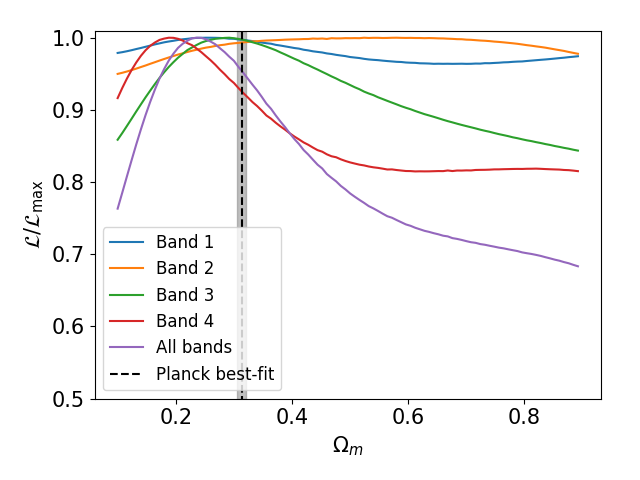
\includegraphics[width=.7\linewidth]{Imagens/profile_ctg_Nmc2e7.png}
	\caption{Normalized $C^{tg}$ likelihood of each band of the 2MASS catalog and combination of all bands' likelihoods. The Planck best-fit for $\Omega_m$ is shown for comparison, the gray band represents represents the 68\% error.}
	\label{fig:likelihood_prof_ctg}
\end{figure}

Figure \ref{fig:likelihood_prof_ctg} shows that the CMB-galaxy cross-correlation data from 2MASS does not significantly constraint the $\Omega_m$ parameter, the likelihoods calculated for every physically meaningful value of $\Omega_m$ are within 70\% of the maximum likelihoods obtained. 

Bands 3 and 4 of 2MASS seem to have a higher constraining capability compared with bands 1 and 2. As shown in Figure \ref{fig:2MASS_selections}, these bands contain galaxies at higher redshifts compared to the other two, which can be interpreted as another indication that using a galaxy catalog containing measurements of galaxies at higher redshifts may lead to a better cross-correlation signal.

Figure \ref{fig:likelihood_prof_ctg+cgg} shows the $C^{tg}+C^{gg}$ joint-likelihood calculated for each of the four bands of the 2MASS catalog, as well as the full 2MASS joint-likelihood of all the bands together. 

\begin{figure}[!htb]
	\centering
	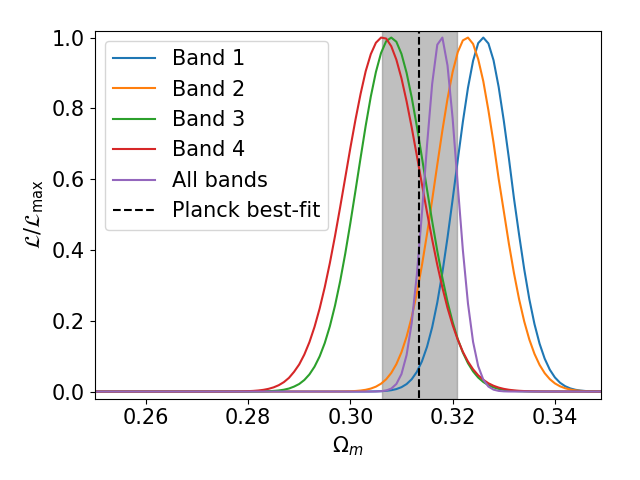
\includegraphics[width=.7\linewidth]{Imagens/profile_allbands_Nmc2e7.png}
	\caption{Normalized $C^{tg}+C^{gg}$ joint-likelihoods for each band of the 2MASS catalog and full joint-likelihood of all bands. The Planck best-fit for $\Omega_m$ is shown for comparison, the gray band represents represents the 68\% error.}
	\label{fig:likelihood_prof_ctg+cgg}
\end{figure}

Simply visualizing the gray band and comparing it with the peaks of the likelihoods indicate that all bands and the full joint-likelihood are compatible with Planck's results. The width of the likelihoods in all bands are similar, showing small differences between the constraining power of each band in this analysis. 

Comparing these results with Figure \ref{fig:likelihood_prof_ctg} shows that $C^{gg}$ has a much higher constraining power over $\Omega_m$ than $C^{tg}$: while Figure \ref{fig:likelihood_prof_ctg+cgg} shows narrow peaks around $0.28 \le \Omega_m \le 0.34$ with nearly null likelihoods outside of this small region, the results for $C^{tg}$ show very high relative likelihood values across all physical values of $\Omega_m$, as previously discussed.

The width of the curves obtained in this project are comparable to the 68\% Planck error for $\Omega_m$, showing that the combination of these two spectra have some constraining power with respect to this parameter. 

\section{Forecast for the Optimized Band}

We have also performed an analysis using synthetic data following the optimized selection function discussed in Chapter \ref{chapter:select_func_optimal}. To do so, we have calculated two cross-correlation spectra: one according to the fiducial $\Lambda$CDM model, and another using $\Omega_m=0.188$, the value that maximizes the likelihood corresponding to band 4 in \ref{fig:likelihood_prof_ctg}. We have used these spectra as datasets with errors equal to that of band 4 of 2MASS. The results of this procedure are shown in Figure \ref{fig:likelihood_band_optimal}.

\begin{figure}[!htb]
	\centering
	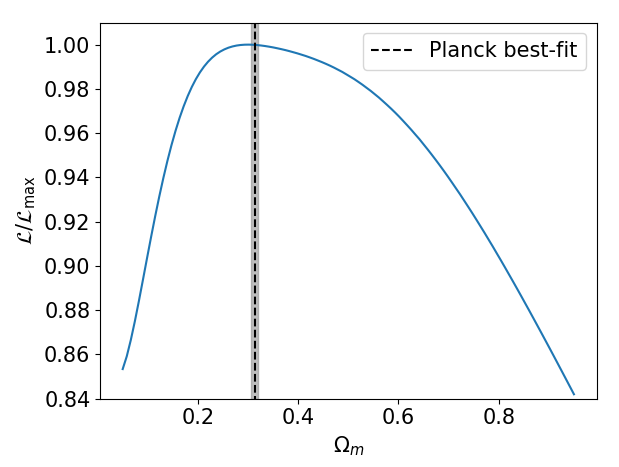
\includegraphics[width=.7\linewidth]{Imagens/profile_BestBand.png}
	\caption{Normalized $C^{tg}$ likelihoods calculated using synthetic data estimated as the theoretical cross-correlation obtained using the idealized band estimated in Chapter \ref{chapter:select_func_optimal} for the selection function. The blue dashed line is calculated with a cross-correlation spectrum generated with $\Omega_m=0.188$ as fiducial value, while the orange curve is calculated using a fiducial $\Lambda$CDM cross-correlation sepctrum with 2MASS', both with errors equal to that of 2MASS' band 4. The Planck best-fit for $\Omega_m$ is shown for comparison, the gray band represents represents its 68\% error.}
	\label{fig:likelihood_band_optimal}
\end{figure}

Despite the fact that both likelihoods calculated from the synthetic data shown in Figure \ref{fig:likelihood_band_optimal} do not have a very strong constraining power, they show some improvement in the $\Omega_m$ constraints compared to the 2MASS' likelihoods, including the combined likelihood, indicating that this idealized survey can in fact make a significant difference in this analysis. 

Another important factor is that this idealized band is deeper than 2MASS, the amount of galaxies measured has a tendency to increase in that situation, reducing the errors, so in this regard it is possible to say the analysis done has been conservative, and the likelihoods could have been improved with more realistic errors.

It is important to remind that, in the analysis made in Chapter \ref{chapter:select_func_optimal}, we have found a parametrization of the selection function that maximizes the likelihood of the theoretical spectrum relative to the null hypothesis of zero cross-correlation spectrum, not the parametrization that improves the constraint power on $\Omega_m$. Despite this, the null hypothesis is a result of $\Omega_m=1$ since the gravitational potentials would not vary in such a universe \cite{ronaldo_inhDE}. In fact, Figure \ref{fig:likelihood_band_optimal} shows that for the optimized band, both likelihoods decrease more rapidily for high values of $\Omega_m$ compared to any of the 2MASS likelihoods.

A similar work has been done in \cite{simillar_ISW_analysis}, in which the authors also analysed the 2MASS+WMAP cross-correlation signal, also finding a preference towards the non-null cross-correlation hypothesis, and studied whether new changes in the data sets -- such deeper galaxy surveys and fainter magnitude limits -- could possibly improve the signal, and reported that even with optimized data sets, the signal would still evade detection in $>10\%$ of cases.

\chapter{Conclusions}\label{chapter:conclusions}

In this work we have studied the possibility of using the integrated Sachs-Wolfe effect as a tool to constrain cosmological parameters. More specifically, we have studied the properties of the cross-correlation spectrum between a CMB temperature map and a galaxy contrast map. The method used to obtain this spectrum from the corresponding maps has already been tested and validated in \cite{Moura-Santos_2016}, as discussed in Chapter \ref{chapter:extracting_correlations_from_data}. The recovered signal is heavily affected by cosmic variance.
%and although the signal was obtained, it was nearly indistinguishable from a zero cross-correlation hypothesis. As discussed, this difficulty arises from the fact the the ISW signal is mostly present at low multipoles, meaning there is a very high irreducible error contribution from cosmic variance. 

In an attempt to solve this, we have first studied if a hypothetical galaxy survey with a tunable selection function could possibly improve the signal in a way that would distinguish it from the null hypothesis (zero cross-correlation). Finally, we have obtained constraints for the $\Omega_m$ parameter using the 2MASS+WMAP data, and did the same with synthetic data corresponding to the idealized galaxy survey discussed before.

In chapter \ref{chapter:select_func_optimal} we have studied the impact of the galaxy redshift distribution -- here called the selection function -- of a catalog in the cross-correlation signal. We have used a certain form of the selection function based on three parameters, and analysed the impact of each parameter in the selection function (see Figure \ref{fig:selection_tripleplot}), which allowed us to control and search for a selection function that improves the cross-correlation signal. In other words, this idealized galaxy catalog would maximize the likelihood function of the cross-correlation data relative to the null hypothesis for which the average cross-correlation is zero for all multipoles. 

We have estimated the redshift at which the Universe started its accelerated expansion and opted to start searching the idealized selection function around that region. To do so, 2D heat maps for the selection function parameters were produced in order to search for regions in the parameter space that might contain a minimum value for the probability of consistency between alternative and null hypotheses. Figure \ref{fig:Triple_ColorPlots} shows one of the most promising regions we have found, from which we have chosen a starting point to run an algorithm to minimize the likelihood function. Despite some promising properties of the idealized parametrization found (see Figure \ref{fig:minimum_properties}), the likelihood ratio at its minimum, i.e. for an optimized survey, is only 3\% smaller than the equivalent ratio calculated using the selection function of band 1 of the 2MASS catalog. In both cases, the cosmological model adopted is $\Lambda$CDM.

In Chapter \ref{chapter:extracting_correlations_from_data}, the matter of how to extract the correlation functions from CMB and galaxy contrast maps was discussed, in which the process developed in \cite{Moura-Santos_2016} was presented alongside the final results of its application to the 2MASS galaxy catalog and the WMAP 9-year CMB intensity (T) maps, which are shown in Figure \ref{fig:correlation_data_final_plots}. The central values with their error bars for the galaxy contrast autocorrelation ($C^{gg}$ in the center column) and CMB-galaxy contrast cross-correlation ($C^{tg}$ in the right column) were used as the input for the analysis of Chapter \ref{chapter:constraints}.

In Chapter \ref{chapter:constraints}, we show cosmological constraints using the ISW effect as manifested through the cross-correlation between the CMB temperature and the galaxy contrast maps. The likelihood functions used are discussed and their profiles are obtained as a function of the $\Omega_m$ parameter, maintaining all other parameters fixed. A full analysis would ideally use these likelihood functions for the MCMC algorithm, resulting in contraints for other cosmological parameters, and possibly even parameters related to alternative dark energy models like the ones shown in Section \ref{sect:dark_energy}, but due to the dominance of cosmic variance at large scales, such constraints would be weak.

Figure \ref{fig:likelihood_prof_ctg} shows the likelihood profiles for all 2MASS bands using only the $C^{tg}$ data, it shows constraints much weaker than those obtained using the joint intensity and polarization TT+EE+TE Planck likelihood. Figure \ref{fig:likelihood_prof_ctg+cgg} shows significantly better contraints are obtained when using the $C^{gg}$ spectrum as a complement to the $C^{tg}$ data. 

We have also used the cross-correlation spectrum for the $\Lambda$CDM fiducial model and the same model with $\Omega_m=0.188$ as a synthetic dataset, with errors equal to that of 2MASS' band 4, to analyse the constraining power of our idealized galaxy catalog -- determined in Chapter \ref{chapter:select_func_optimal} -- would have on $\Omega_m$. We discussed how the uncertainties used might be overestimated due to deeper surveys having higher galaxy counts, thus lower uncertainties, and how the uncertainties dominate the region relevant to the analysis. Figure \ref{fig:likelihood_band_optimal} shows a significant improvement in the results, even when compared with the joint likelihood results, indicating that such a galaxy survey can significantly improve the ISW signal.

It is also important to highlight the work made in \cite{simillar_ISW_analysis}, in which the authors have analysed if changes in the data, including changes in the redshift distribution of the galaxies of the catalog used, would significantly improve the ISW signal. Despite exploring very different changes in the selection function compared to the ones made in this project, and other idealized properties for the data, it was also reported that the ISW signal would still evade detection in $>10\%$ of cases.

In \cite{cross_corr:Planck}, the authors were able to find a CMB-galaxy cross-correlation signal with significance level of $4\sigma$ combining different matter tracers, the main ones being Planck's convergence lensing maps (Kappa) with a detection level of $3.2\sigma$ and radio sources from the NVSS galaxy catalogue\cite{NVSS} with $2.6\sigma$. These two datasets provide data on very far away galaxies, with redshifts up to $z=5$, and both have a good sky coverage, hinting that deeper surveys can yield better signals overall.

Ideally, detecting the ISW signal should consist of a combination of methods that are complementary, the angular cross-correlation spectrum studied here is a powerful one, but clearly its potential needs to be enhanced with the use of other tracers. The results of reference \cite{cross_corr:Planck} further evinces the importance of combining different tracers with correspondingly different bias factors and redshift distributions.

%We have attempted to reduce the cosmic variance contribution to the errors with reasonable success, the constraints obtained for $\Omega_m$ have improved significantly with this analysis, but are still very wide, and require complimentary data for high quality cosmological constraints. 

%Comparing the results obtained here with other references, especially \cite{cross_corr:Planck}, leads us to think that, for an analysis using galaxy maps as tracers, deeper surveys such as NVSS -- which contains galaxies up to $z=5$, significantly deeper than both 2MASS and our idealized galaxy distribution -- might be one of the most relevant choices for an improved signal. This also means that running the algorithm discussed in Chapter \ref{chapter:select_func_optimal} with different parametrizations for the selection function, and choosing a deeper distribution as the starting point of the algorithm, might lead to optimal galaxy catalogs that are even better at reducing the influence of cosmic variance.

%Going back to the MCMC chains and studying the influence of the cross-correlation spectra discussed so far for a full cosmological analysis could help us understand the influence of this data in other cosmological parameters, and how much the constraints on $\Omega_m$ would change. A more detailed study of the MCMC chains could possibly allow us to find way to make it run in a more viable time frame, and that could be coupled with a better optimization of the integration algorithm responsible for the calculation of the correlation functions.

%We also highlight the work made in \cite{growth_constraint}, it uses a parametrization for the linear growth function $D(z)$ in \cite{growth_model}

%\begin{equation}\label{growth_func_new}
%	\dv{\ln{D(a)}}{\ln{a}}=\Omega_m^\gamma (a),
%\end{equation}

%\noindent where $\gamma$ is the growth index. It has been shown that using standard general relativity applied to a flat metric should lead to $\gamma\approx 0.55$, but when analysing both CMB data and some large scale structure datasets, the authors report a value of $\gamma=0.639\substack{+0.024 \\ -0.025}$, excluding the value of $\gamma=0.55$ at a statistical significance of $3.7\sigma$. They have also shown that using $\gamma$ as a free parameter can resolve the two main tensions in cosmology: The $\sigma_8$ tension and the Hubble tension. Testing how the results shown in this work would behave in such a model can be an interesting path forward, since the growth of structure during the dark energy dominated era is so important to the ISW.

\appendix

\newpage

\begin{center}
\thispagestyle{empty}
\vspace*{\fill}
\Huge{Appendices}
\vspace*{\fill}
\end{center}

\iffalse %multiline comment
\chapter{Fourier Space}\label{appendix:FourierSpace}

Say we have a function $\delta(\mathbf{x},t)$ that follows a linear partial differential equation, such as

\begin{equation}\label{Four_Space:example_diff_eq}
	\pdv[2]{}{t} \delta(\mathbf{x},t) +f(t)\delta(\mathbf{x},t) + g(t)\nabla^2\Psi(\mathbf{x},t)=0.
\end{equation}

Notice that the terms in the equation are only time dependent. These properties make this equation suitable to use a Fourier transform to analyse it: If we take

\begin{equation}
	\delta(\mathbf{k},t)=\int d^3x e^{-i\mathbf{k}\cdot \mathbf{x}}\delta(\mathbf{x}),
\end{equation}

\noindent to be the Fourier transform of $\delta(\mathbf{x},t)$, then space derivatives of $\delta(\mathbf{x},t)$ become simple multiplicative terms:

\begin{equation}
	\pdv{\delta(\mathbf{x},t)}{x^i}=ik_i\delta(\mathbf{k},t).
\end{equation}

Because of that, if one takes the Fourier transform of the entire equation, it becomes simplified:

\begin{equation}\label{Four_Space:final_eq}
	\pdv[2]{}{t}\delta(\mathbf{k},t)+f(t)\pdv{}{t}\delta(\mathbf{k},t)-g(t)k^2\Psi(\mathbf{k},t)=0.
\end{equation}

Fourier space is commonly used to study functions related to waves, and in that case $\mathbf{k}$ corresponds to the wavevector of that signal. In that context, it is useful to define the spectral density.

Falar sobre espaço de fourier
Falar do conceito de spectral density/power spectrum
\fi

\chapter{Transition Redshift for a Dark Energy Dominated Universe}\label{app:dark_energy_era}

We will start defining the decelerating parameter $q(a)$

\begin{equation}\label{def:decelerating_parameter}
	q(a)\equiv -\frac{\ddot{a}a}{\dot{a}}.
\end{equation} 

An expression for this parameter can be determined by dividing the second Friedmann equation (equation \eqref{fried_second_eq}) by the first Friedmann equation (equation \eqref{fried_first_eq}) and multiplying the result by minus one:

\begin{equation}\label{app_DE:step1}
	q(a)=-\frac{\ddot{a}a}{\dot{a}}=\frac{1}{2}\left(\frac{\rho+3P}{\rho}\right).
\end{equation}

We will use $\rho=\rho_m+\rho_\text{de}+\rho_r$ and assume $\Omega_k=0$ (see Table \ref{tab:rhos&Omegas}), meaning $\rho=\rho_\text{crit}$, so equation \eqref{app_DE:step1} becomes

\begin{equation}\label{app_DE:step2}
	q(a)=\frac{1}{2}\left(\frac{\rho_m+\rho_\text{de}+\rho_r+3P}{\rho_\text{crit}}\right).
\end{equation}

As discussed in Section \ref{subsect:Ch2_Energy_Content}, it is commonly assumed that $P_s=w_s\rho_s$, so equation \eqref{app_DE:step2} becomes

\begin{equation}\label{app_DE:step3}
	q(a)=\frac{1}{2}\left[\frac{\rho_m+\rho_\text{de}+\rho_r+3(w_m\rho_m+w_r\rho_r+w_\text{de}\rho_\text{de})}{\rho_\text{crit}}\right].
\end{equation}

We can use the values shown in Table \ref{tab:rhos&Omegas} and use the definition of $\Omega_s$ (equation \eqref{eq:Omega_def}) to obtain

\begin{equation}\label{q(a)_expression}
	q(a)=\frac{1}{2}\Omega_m(a)+\Omega_r(a)+\frac{3w_\text{de}+1}{2}\Omega_\text{de}(a)
\end{equation}

Using the evolution equations for $\Omega_s(a)$ in terms of $\Omega_s=\Omega_s(a_0)$ shown in \cite{dark_energy_era}:

\begin{align}\label{evolution_eqs}
	\Omega_m(a)&=\frac{\Omega_m}{E(a)}a, & \Omega_r(a)&=\frac{\Omega_r}{E(a)}, & \Omega_\text{de}&=\frac{\Omega_\text{de}}{E(a)}a^{1-3w_\text{de}},
\end{align}

\noindent where $E(a)=\Omega_r+\Omega_m a +\Omega_\text{de}a^{1-3w_\text{de}}$, and taking $\Omega_r=0$, we obtain

\begin{equation}\label{app_DE:step4}
	q(a)=\frac{1}{2}\left[\frac{\Omega_m a+(1+3w_\text{de})\Omega_\text{de}a^{1-3w_\text{de}}}{\Omega_m a +\Omega_\text{de}a^{1-3w_\text{de}}}\right].
\end{equation}

To find the scale factor in which the expansion's acceleration becomes positive, we can simply impose that $q(a^*)=0$. Then we can change variables using $a^*=1/(1+z^*)$ and solve for $z^*$, obtaining

\begin{equation}
	z^*=\left[-(1+3w_\text{de})\frac{\Omega_\text{de}}{\Omega_m}\right]^{-\frac{1}{3w_\text{de}}}-1
\end{equation}

\chapter{CMB-galaxy Cross-correlation Formulae}\label{app:correlations_demo}

Expanding the definition of $C_\ell^{TT}$ given in \eqref{def:autocorrelation} one can show that \cite{dodelson2020modern}:

\begin{equation}\label{demo:Start_eq}
	C_\ell^{tt}=\frac{2}{\pi}\int dk k^2P(k)\left|\frac{\Theta_\ell(k,\eta_0)}{\delta(k,\eta_0)}\right|^2.
\end{equation}

Similar expressions can be found for $C_\ell^{tg}$ and $C_\ell^{gg}$, we will focus the demonstration on the temperature autocorrelation case.

Using the ISW term of equation \eqref{ch2:Thetal_approx}

\begin{equation}
	\Theta_\ell^{\text{ISW}}(k,\eta_0)=\int_0^{\eta_0} d\eta e^{-\tau}[\Psi'(k,\eta)-\Phi'(k,\eta)]j_\ell[k(\eta_0-\eta)],
\end{equation}

\noindent with $e^{-\tau}\approx 1$ since, as shown, the ISW effect is only relevant at large scales\footnote{The Planck best-fit for the optical depth in the present is $\tau=0.054\pm 0.007$}. So

\begin{equation}\label{appA:step1}
	\Theta_\ell^{\text{ISW}}(k,\eta_0)=\int_0^{\eta_0} d\eta \dv{}{\eta}\left[\Psi(k,\eta)-\Phi(k,\eta)\right]j_\ell[k(\eta_0-\eta)],
\end{equation}

Using the definition of $\eta$ in \eqref{def:conformal_time}

\begin{equation}
	\eta=\int_0^t \frac{dt}{a(t)}=\int_0^a\frac{da'}{a'^2H(a')}=\int_{z}^\infty \frac{dz'}{H(z)},
\end{equation}

\noindent we can do a change in variables of the integral to redshift. Since

\begin{equation}
	\eta_0-\eta=\int_0^\infty \frac{dz'}{H(z')}-\int_z^\infty \frac{dz'}{H(z')}=\int_z^\infty \frac{dz'}{H(z')}=\chi(z),
\end{equation}

\noindent where $\chi(z)$ is the comoving distance, equation \eqref{appA:step1} becomes

\begin{equation}
	\Theta_\ell^\text{ISW}(k,z=0)=\int_0^\infty dz \dv{}{z}\left[\Psi(k,z)-\Phi(k,z)\right]j_\ell[k\chi(z)].
\end{equation}

At late times, we can neglect anisotropic stress, taking $\Psi\approx \Phi$, therefore

\begin{equation}
	\Theta_\ell^\text{ISW}(k,0)=-2\int_0^\infty dz \dv{\Phi}{z}j_\ell [k\chi(z)].
\end{equation}

Finally, we can use the Poisson equation

\begin{equation}
	\Phi(k,z)=\frac{3}{2}\Omega_m \left(\frac{H_0}{k}\right)^2(1+z)\delta(k,z),
\end{equation}

\noindent to show that

\begin{equation}
	\delta(k,0)=\frac{2}{3\Omega_m}\left(\frac{k}{H_0}\right)^2\Phi(k,0).
\end{equation}

With this:

\begin{equation}
	\frac{\Theta_\ell(k,\eta_0)}{\delta(k,\eta_0)}=\frac{\Theta_\ell(k,z=0)}{\delta(k,z=0)}=-3\Omega_m\left(\frac{H_0}{k}\right)^2\int_0^\infty dz \dv{}{z}\left[\frac{\Phi(k,z)}{\Phi(k,0)}\right]j_\ell[k\chi(z)].
\end{equation}

Cosmologists define the growth function $D(z)$ as

\begin{equation}
	\frac{\Phi(k,a)}{\Phi(k,1)}\equiv\frac{D(a)}{a}=(1+z)D(z)=\frac{\Phi(k,z)}{\Phi(k,0)},
\end{equation}

so

\begin{equation}
	\frac{\Theta_\ell(k,\eta_0)}{\delta(k,\eta_0)}=-3\Omega_m\left(\frac{H_0}{k}\right)^2\int_0^\infty \dv{(1+z)D(z)}{z}j_\ell[k\chi(z)].
\end{equation}

Using this result, equation \eqref{demo:Start_eq} in terms of redshift instead of $\eta$ becomes

\begin{equation}\label{AppA:eq_final}
	C_\ell^{tt}=\frac{2}{\pi}\int_0^\infty dk k^2P(k)|W_\ell^t|^2
\end{equation}

\noindent with 

\begin{equation}
	W_\ell^t=-3\Omega_m\left(\frac{H_0}{k}\right)^2\int_0^\infty \dv{(1+z)D(z)}{z}j_\ell[k\chi(z)].
\end{equation}

Equation \eqref{appA:step1} expresses the present contribution of the late ISW  effect to the CMB temperature autocorrelation spectrum.

\end{spacing}
\endgroup

\printbibliography

\end{document}
